\documentclass[hidelinks,12pt,a4paper,twoside]{article}

%% ==================================================================
%%%% Preamble
%% ==================================================================
%% ==================================================================
%%%% Packages
%% ==================================================================
\usepackage[a4paper]{geometry}
\usepackage[utf8]{inputenc}
\usepackage[ngerman]{babel}
\usepackage[T1]{fontenc}
\usepackage{newpxtext,newpxmath}
\usepackage[hidelinks]{hyperref}
\usepackage{amsmath,amssymb,amstext}
\usepackage{mathtools}
\usepackage[backend=biber,citestyle=verbose, bibstyle=verbose]{biblatex}
\usepackage[babel,german=guillemets]{csquotes}
\usepackage{fancyhdr}
\usepackage{microtype}
\usepackage{graphicx}
\usepackage{float}
\usepackage{minted}
\usepackage{acronym}
\usepackage{booktabs}
\usepackage{multirow}
\usepackage{pgf}
%\usepackage{pgfplots}
\usepackage{siunitx}
\usepackage{xcolor,mdframed}
\usepackage{lipsum}
\usepackage{listings,chngcntr} 			% kapitelweise Nummerierung für Codeabschnitte
\usepackage{listings,xcolor} 				% ermöglicht das Einbinden von Codesegmenten
\usepackage{listingsutf8} 					% ermöglicht das Einbinden von Codesegmenten
\usepackage{url}
\usepackage{subfigure}


%% ==================================================================
%%%% General Document Settings
%% ==================================================================
\linespread{1.5}
\parindent 0ex

\bibliography{bibliography.bib}

\graphicspath{ {./images/} }

\setcounter{tocdepth}{4}
\setcounter{secnumdepth}{4}

\sisetup{locale = DE}

\raggedbottom % Allow ragged page bottoms

\renewcommand{\familydefault}{\sfdefault} % Arial ähnliche Schriftart

\def \sectionauthors {Philipp Kraft, Dennis Köb und Samuel Bleiner}


%% ==================================================================
%%%% Fancy Header Settings
%% ==================================================================
\pagestyle{fancy}
\fancyhead{}
\fancyfoot{}
\fancyhead[L]{\hspace{0.2cm} 
\includegraphics[height=1.04cm]{htl_rankweil_logo.png}}
\fancyhead[C]{\textbf{HTL Rankweil}
  \\[0.05in]
  \footnotesize{Höhere Lehranstalt für Elektronik und Technische Informatik}}
\fancyhead[R]{
\includegraphics[height=1.04cm]{htl_logo.png} \hspace{0.2cm}}

\fancyfoot[LE,RO]{\thepage}
\fancyfoot[LO,RE]{2020/21 Advanced Parking Monitoring}

\setlength{\headheight}{34pt}
\renewcommand{\footrulewidth}{0.4pt}


%% ==================================================================
%%%% Listings Settings
%% ==================================================================
\renewcommand{\listingscaption}{Code}
\renewcommand{\listoflistingscaption}{Codeverzeichnis}

\definecolor{backcolour}{gray}{0.95}

\setminted
{
  mathescape,
  bgcolor = backcolour,
  linenos = true,
  numbersep = 5pt,
  gobble = 2,
  framesep = 2mm,
  numberblanklines = true,
  breaklines = true,
  numberblanklines = true
}


%% ==================================================================
%%%% Important Info Block
%% ==================================================================
\newenvironment{important}[1][]{%
  \begin{mdframed}[%
      backgroundcolor={red!15}, hidealllines=true,
      skipabove=0.7\baselineskip, skipbelow=0.7\baselineskip,
      splitbottomskip=2pt, splittopskip=4pt, #1]%
    \makebox[0pt]{% ignore the withd of !
      \smash{% ignor the height of !
        \fontsize{32pt}{32pt}\selectfont% make the ! bigger
        \hspace*{-19pt}% move ! to the left
        \raisebox{-2pt}{% move ! up a little
          {\color{red!70!black}\sffamily\bfseries !}% type the bold red !
        }%
      }%
    }%
    }{\end{mdframed}}


%% ==================================================================
%%%% Frontmatter, Mainmatter and Backmatter
%% ==================================================================
\def\frontmatter{%
  \pagenumbering{roman}
  \setcounter{page}{1}
  \renewcommand{\thesection}{\Roman{section}}
}%

\def\mainmatter{%
  \pagenumbering{arabic}
  \setcounter{page}{1}
  \setcounter{section}{0}
  \renewcommand{\thesection}{\arabic{section}}
}%

\def\backmatter{%
  \setcounter{section}{0}
  \renewcommand{\thesection}{\Alph{section}}
}%



\begin{document}

%% ==================================================================
%%%% Main Content
%% ==================================================================
\begin{titlepage}
  \begin{center}
    \vspace*{1cm}
    \large{\textbf{HTL Rankweil}}\\
    \large{\textbf{5AHEL 2020/21}}
    \vfill
    \line(1,0){400}\\[1mm]
    \huge{\textbf{DIPLOMARBEIT}}\\[3mm]
    \large{\textbf{Advanced Parking Monitoring (APM)}}\\[1mm]
    \line(1,0){400}\\
    \vfill
    Philipp Kraft, Dennis Köb und Samuel Bleiner\\[3mm]
    Dipl.-Ing. Christoph Stüttler \\[6mm]
    \today, Rankweil
  \end{center}
\end{titlepage}

%\pagebreak
%\thispagestyle{empty}
%\hspace{0pt}
%\vfill
%\begin{figure}[h]
%  \centering
%  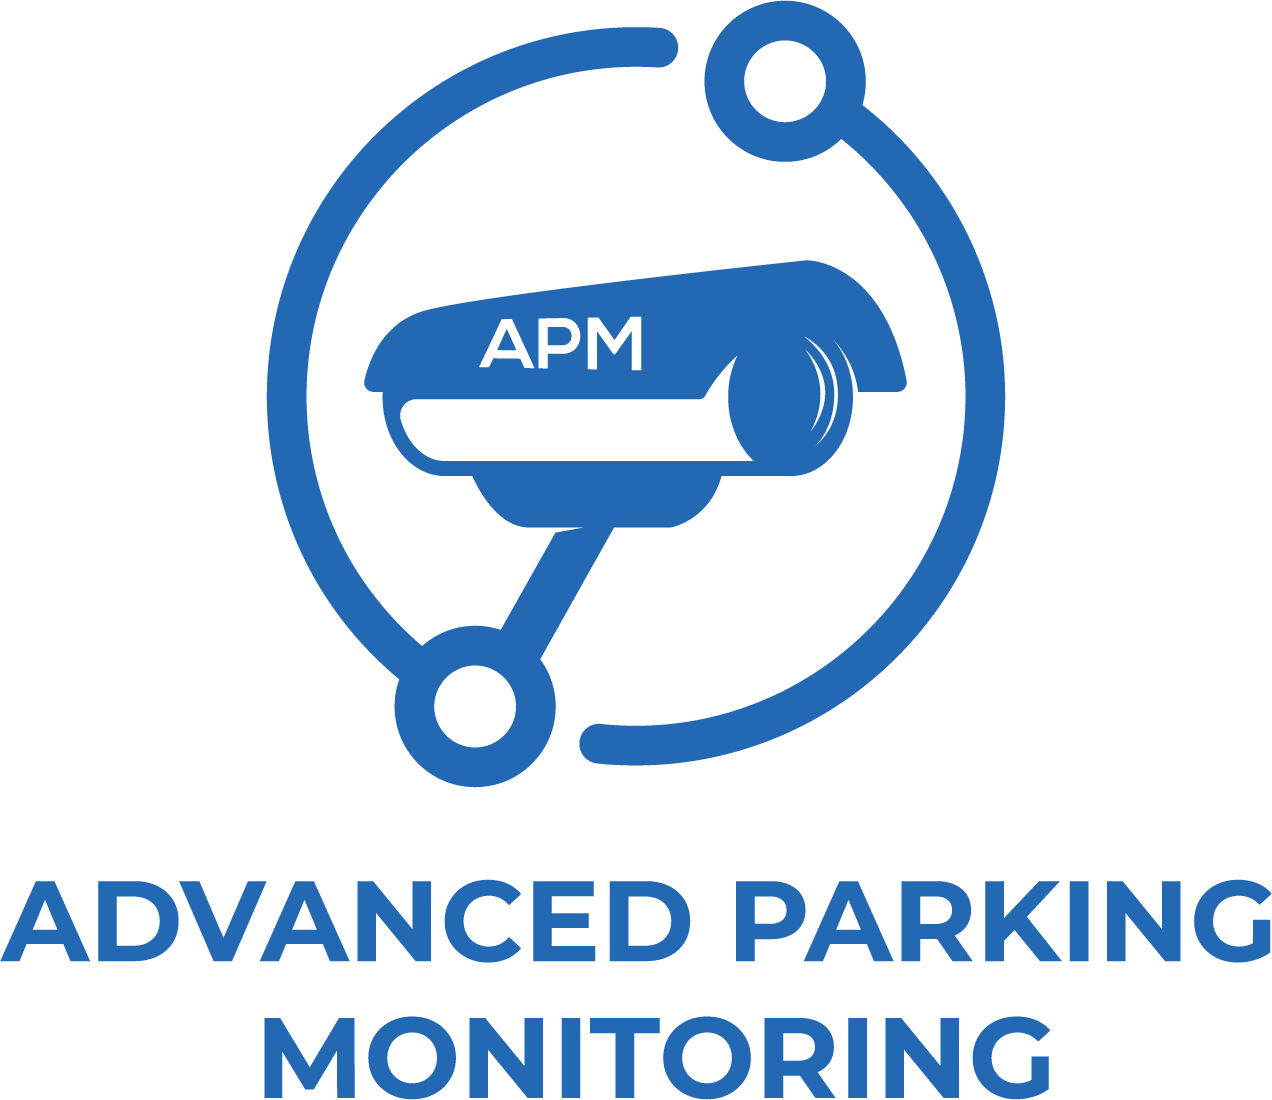
\includegraphics[width=\textwidth]{APM_Logo_Transparent.png}
%  \label{fig:apm_logo}
%\end{figure}
%\vfill
%\hspace{0pt}


\fancyfoot[LO,RE]{\sectionauthors}

\frontmatter

\section*{Eidesstattliche Erklärung}
\addcontentsline{toc}{section}{Eidesstattliche Erklärung}
Ich erkläre an Eides statt, dass ich die vorliegende Diplomarbeit selbständig
und ohne fremde Hilfe verfasst, andere als die angegebenen Quellen und
Hilfsmittel nicht benutzt und die den benutzten Quellen wörtlich und inhaltlich
entnommenen Stellen als solche erkenntlich gemacht habe.

\vspace*{1cm}
Rankweil, 20. April 2021

\vspace*{2cm}


\begin{center}
  \begin{tabular}{cp{2em}c} \hspace{6cm} \\\cline{1-1}\cline{3-3} \\[-3mm]
    {\footnotesize Philipp Kraft}
  \end{tabular}

  \vspace*{1cm}

  \begin{tabular}{cp{2em}c} \hspace{6cm} \\\cline{1-1}\cline{3-3} \\[-3mm]
    {\footnotesize Dennis Köb}
  \end{tabular}

  \vspace*{1cm}

  \begin{tabular}{cp{2em}c} \hspace{6cm} \\\cline{1-1}\cline{3-3} \\[-3mm]
    {\footnotesize Samuel Bleiner}
  \end{tabular}

\end{center}


\pagebreak


\section*{Kurzfassung}
\addcontentsline{toc}{section}{Kurzfassung}
\lipsum[1-2]
\pagebreak


\section*{Abstract}
\addcontentsline{toc}{section}{Abstract}
\lipsum[1-2]
\pagebreak


\section*{Vorwort}
\addcontentsline{toc}{section}{Vorwort}
In den Jahren unserer Ausbildungszeit ist uns immer wieder aufgefallen, dass
öffentliche gebührenpflichtige Parkplätze kaum moderne technische Innovationen für Zutritt und Abrechnung nutzen.
Daraufhin haben wir uns durch zusätzliche Anregung von unserem
Betreuungslehrer Dipl.-Ing. Christoph Stüttler dazu entschieden, diese Thematik
für unsere Diplomarbeit heranzuziehen.\\

Diese Diplomarbeit soll aufzeigen, wie eine modernes System zur
Parkplatzverwaltung aussehen könnte. Es werden in dieser Arbeit verschiedene
Themenbereiche wie Webinterfaces, künstliche Intelligenz und Mikrocontroller
behandelt.
\pagebreak


\section*{Danksagung}
\addcontentsline{toc}{section}{Danksagung}
Mit dieser Seite wollen wir uns bei allen Personen bedanken die uns zum Erfolg unserer Diplomarbeit geführt haben. 
Wir bedanken uns ausdrücklich bei unserem Betreuungslehrer Dipl.-Ing. Christoph Stüttler für seine fachliche Expertise sowie für alle kreativen Ratschläge während des 
gesamten Betreuungszeitraumes. \\

Unser hauptsächlicher Dank gilt der Firma Omicron für die finanzielle Unterstützung ohne welche die Diplomarbeit in dieser Form nicht existieren würde.\\

Ein herzliches Dankeschön geht an unsere Eltern für ihre Hilfe und für ihren Beistand während unserer gesamten Ausbildungszeit.
\pagebreak


\mainmatter
\setcounter{page}{1}


\tableofcontents
\pagebreak


\section{Projektteam}
\begin{figure}[htbp]
  \centering
  \begin{minipage}[t]{0.35\linewidth}
      \centering
      
\includegraphics[width=\linewidth]{Philipp.png}
      \caption*{\textbf{Philipp Kraft}\\ \href{mailto:mail@philipp-kraft.com}{E-Mail: Mail@Philipp-Kraft.com}}
  \end{minipage}
  \hfill
  \begin{minipage}[t]{0.35\linewidth}
      \centering
      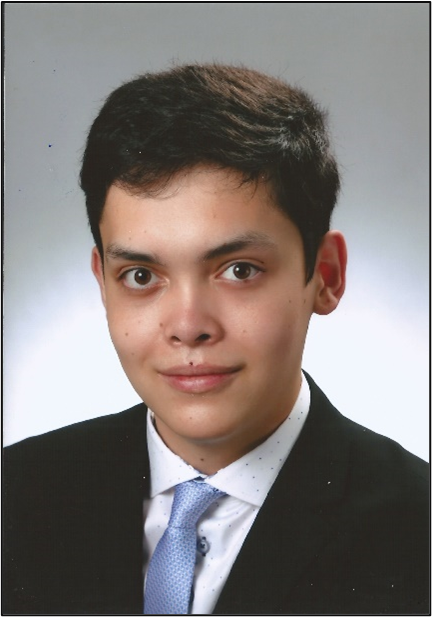
\includegraphics[width=\linewidth]{Dennis.png}
      \caption*{\textbf{Dennis Köb}\\ \href{mailto:dennis.koeb@gmail.com}{E-Mail: Dennis.Koeb@gmail.com}}
  \end{minipage}
\end{figure}

\begin{figure}[H]
  \centering
  \frame{
\includegraphics[width=0.35\linewidth]{Samuel.png}}
  \caption*{\textbf{Samuel Bleiner}\\ \href{mailto:bleiner.samuel@gmail.com}{E-Mail: Bleiner.Samuel@gmail.com}}
\end{figure}
\pagebreak


\section{Projektbetreuer}
\begin{figure}[H]
  \centering
  \frame{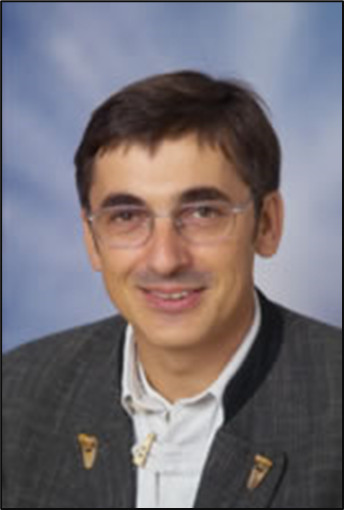
\includegraphics[width=0.35\linewidth]{stu.png}}
  \caption*{\textbf{Dipl.-Ing. Christoph Stüttler}\\ \href{mailto:christoph.stuettler@ht-rankweil.at}{E-Mail: Christoph.Stuettler@ht-rankweil.at}}
\end{figure}

\section{Projektsponsor}
\begin{figure}[H]
  \centering
  
\includegraphics[width=0.7\linewidth]{omicron.pdf}
  \caption*{\textbf{OMICRON electronics GmbH}\\ Oberes Ried 1, 6833 Klaus\\ Telefon: +43 59495}
\end{figure}
\pagebreak


%\section{Auftragnehmer}
%\pagebreak


\section{Projektplanung}
Die Projektplanung ist der wichtigsten Teil des Projektmanagements. Die
Rahmenbedingungen für das Projekt wurden bereits beim Antrag der Diplomarbeit
festgelegt.

\subsection{OpenProject}
Für das Projektmanagement wird die Softwareanwendung
OpenProject\footnote{https://www.openproject.org} verwendet. Der Vorteil dieser
Software ist, dass diese nicht wie eine normale Desktop-Anwendung lokal auf dem
Rechner des Benutzers läuft, sondern auf einem Server. Ein weiterer Vorteil
davon ist, dass das kollaborative arbeiten stark vereinfacht wird. OpenProject
bietet die Möglichkeit die Anwendung in der eigenen Infrastruktur zu
installieren und somit eine vollständige Kontrolle über die eigenen Daten.

\subsection{Phasen}
Die gesamte Projektplanung ist in vier Phasen aufgeteilt:

\begin{itemize}
  \item \textbf{Themenfindungsphase}\\
  In der Themenfindungsphase geht es um das Finden des expliziten Themas, dabei
  werden die Rahmenbedingungen mit dem Betreuer festgelegt.
  \item \textbf{Planungsphase}\\
  In der Planungsphase werden Arbeitspakete erstellt und den einzelnen
  Mitgliedern des Projektes zugeteilt.
  \item \textbf{Entwicklungsphase}
  Die Entwicklungsphase ist der längste und wichtigste Teil des Projekts, dabei
  werden alle Arbeitspakete so gut wie möglich abgearbeitet.
  \item \textbf{Abschlussphase}
  In der Abschlussphase geht es um das Schreiben der Diplomarbeit so wie letzte
  technische Feinschliffe in der Software und Hardware.
\end{itemize}
\subsection{Arbeitspakete}
Grundsätzlich sind die Arbeitspakete in drei Themenbereiche aufgeteilt:

\begin{itemize}
  \item Kennzeichenerkennung (Samuel)
  \item Fahrzeugerkennung (Dennis)
  \item Webinterface (Philipp)
\end{itemize}

\begin{figure}[H]
  \centering
  \frame{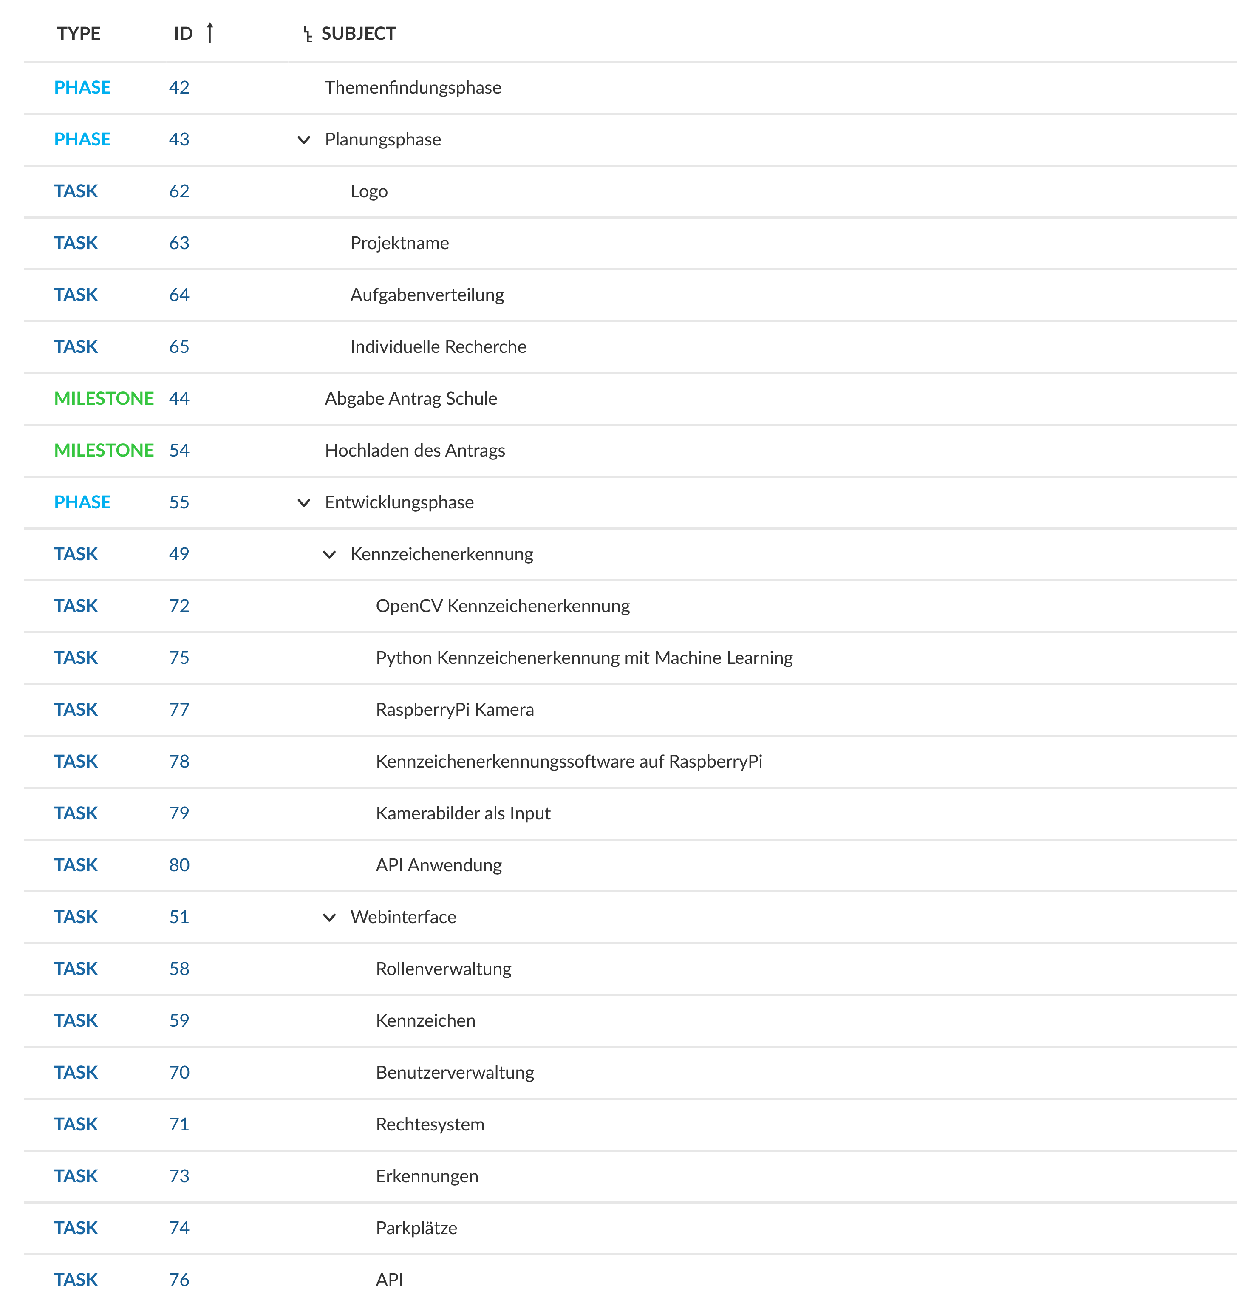
\includegraphics[width=1\linewidth]{arbeitspakete_1.pdf}}
  \caption{Arbeitspakete Teil 1}
\end{figure}

\begin{figure}[H]
  \centering
  \frame{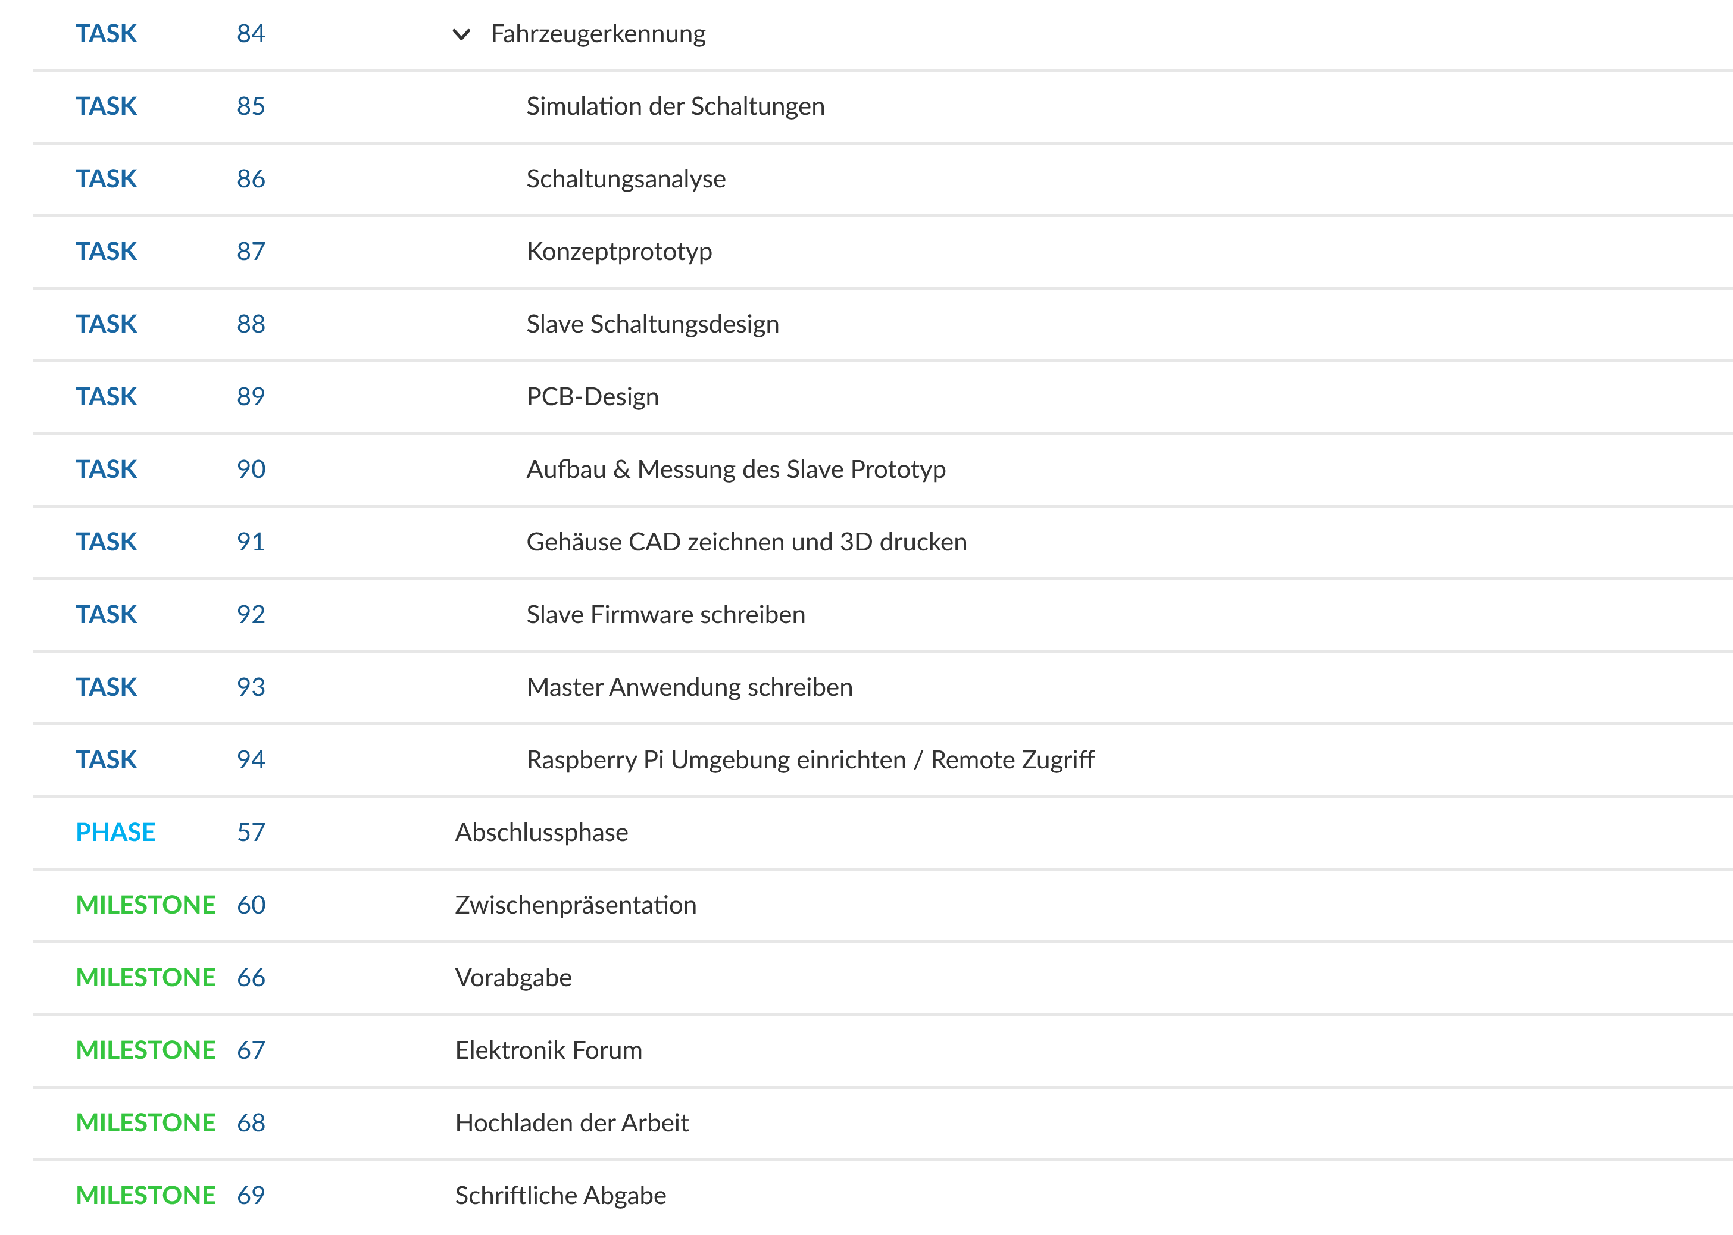
\includegraphics[width=1\linewidth]{arbeitspakete_2.pdf}}
  \caption{Arbeitspakete Teil 2}
\end{figure}

\subsection{Gantt-Diagramm}
Gantt-Diagramme oder Balkenplan sind spezielle Balkendiagramme um verschiedene
Arbeitspakete oder Aktivitäten auf einer Zeitachse darzustellen.

\clearpage \newpage
\begin{sidewaysfigure}[htbp]
  \centering
  \frame{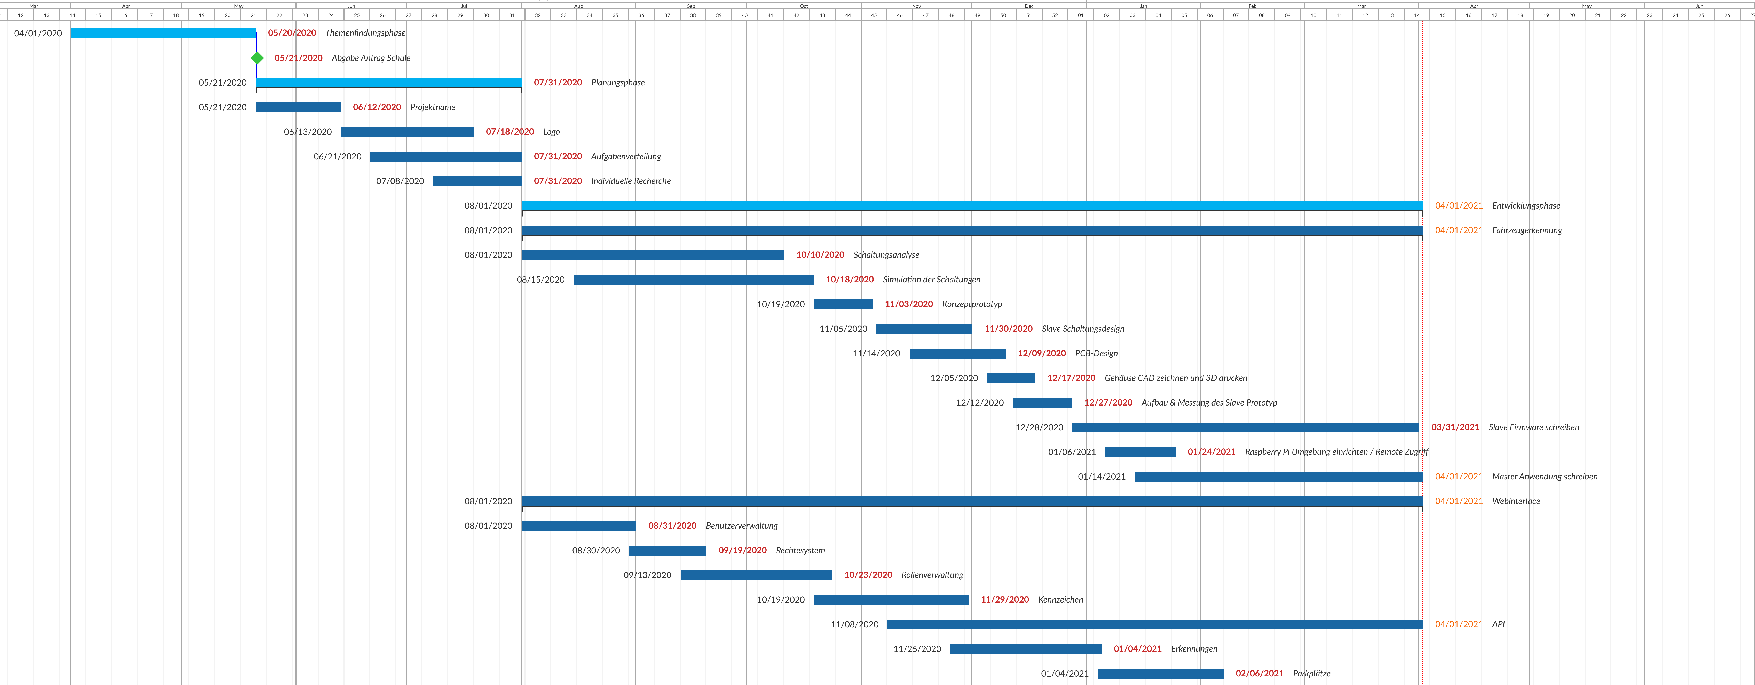
\includegraphics[width=1\linewidth]{gantt_1.pdf}}
  \caption{Gantt-Chart Teil 1}
\end{sidewaysfigure}

\begin{sidewaysfigure}[htbp]
  \centering
  \frame{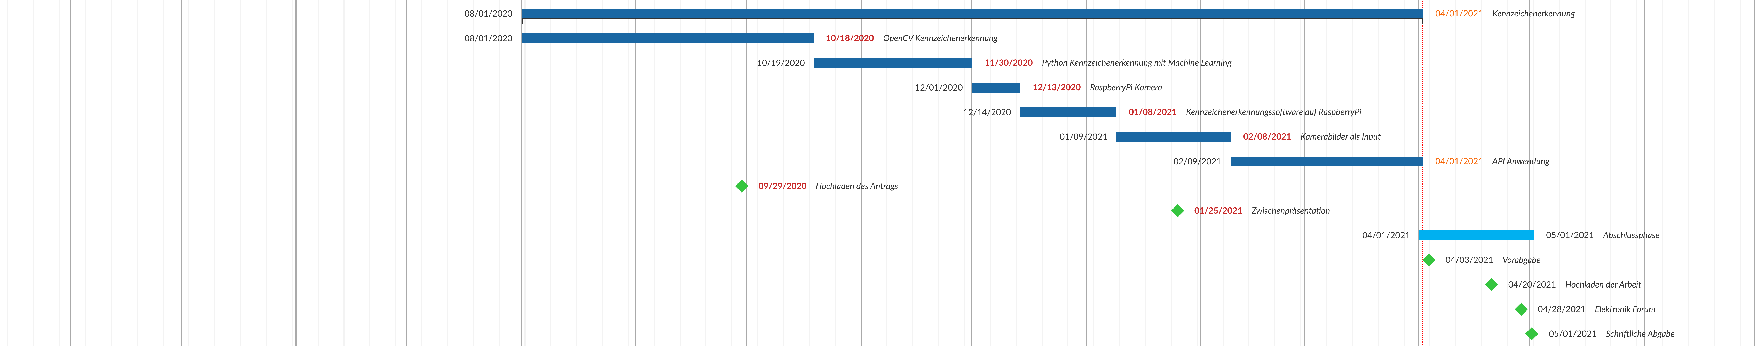
\includegraphics[width=1\linewidth]{gantt_2.pdf}}
  \caption{Gantt-Chart Teil 2}
\end{sidewaysfigure}
\clearpage

\subsection{Zeitaufwendungen}

Die Dokumentation der Zeitaufwendungen erfolgt über ein
Tabellenkalkulationsprogramm, dabei wird folgendes dokumentiert:

\begin{itemize}
  \item Datum
  \item Typ
  \item Beschreibung
  \item Aufwand in Stunden
\end{itemize}

Die komplette Übersicht der aufgewendeten Stunden ist im Anhang ersichtlich.

\begin{table}[H]
  \centering
  \begin{tabular}{@{}ll@{}}
  \toprule
  \multicolumn{2}{c}{\textbf{Zeitaufwendungen}} \\ \midrule
  Philipp Kraft             & 181.5 h           \\
  Dennis Köb                & 177 h             \\
  Samuel Bleiner            & 131.5 h           \\ \midrule
  Gesamtaufwand:            & 490 h             \\ \bottomrule
  \end{tabular}
  \caption{Zeitaufwendungen Übersicht}
\end{table}
\pagebreak


%\section{Rechtliches}
%\pagebreak


\section{Einleitung}
\lipsum[1-2]
\pagebreak


%\section{Projektantrag}
%\input{sections/9_projektantrag.tex}
%\pagebreak


\section{Kennzeichenerkennung}
\def \sectionauthors {Samuel Bleiner}
\subsection{Einleitung}
Der Teil der Kennzeichenerkennung beschäftigt sich damit, aus aufgenommenen Fotos der einfahrenden und ausfahrenden Fahrzeuge, 
das Kennzeichen auszulesen und dieses an die Datenbank zu senden. Dies wird benötigt damit es möglich ist zu bestimmen welches 
Fahrzeug sich im Moment auf dem Parkplatz befindet. Zudem kann dadurch jedes Fahrzeug eindeutig identifiziert werden, da das Kennzeichen 
einzigartig sein muss.  In Zusammenhang mit der Datenbankverwaltung können so auch bestimmte Kennzeichen definiert werden, welche anders 
behandelt werden als andere Kennzeichen. Ein Beispiel dafür wäre kostenloses Parken für den Parkplatzbesitzer oder auch gesperrte Kennzeichen, 
bei welchen der Parkplatzbetreiber eine Benachrichtigung bekommt, wenn sich diese auf dem Parkplatz befinden. Die Verbindung zur Datenbank 
erfolgt über eine eigene API, mit welcher die Daten schnell und einfach übertragen werden können. Um das Programm für die Kennzeichenerkennung 
zu realisieren werden sowohl bewährte Bildverarbeitungsalgorithmen eingesetzt als auch neuronale Netze, welche sich in den Bereich des 
maschinellen Lernens einordnen lassen, wodurch die Genauigkeit gesteigert werden kann. Zusätzlich wird für das komplette Modul ein Gehäuse 
gefertigt in welchem die Elektronik fest verbaut werden kann und trotzdem die Möglichkeit zu weiteren Verbesserungen ermöglicht.

\subsection{Anforderungen}
Das Modul für die Kennzeichenerkennung muss einige Anforderungen erfüllen, um für seinen Einsatzzweck bestmöglich geeignet zu sein.\\

Als Erstes muss die Software einige Anforderungen erfüllen. Sie muss eine hohe Erkennungsgenauigkeit erreichen, um in möglichst jedem einzelnen Fall 
ein korrektes Ergebnis zu liefern. Um diese Genauigkeit zu erreichen werden mehrere Modelle für maschinelles Lernen verwendet, mit welchen 
eine bessere Genauigkeit als mit anderen Methoden erreicht werden kann. Die Geschwindigkeit ist hingegen ein nicht ganz so wichtiger Punkt, 
da Fahrzeuge für eine erfolgreiche Erkennung nicht zu schnell fahren dürfen, um eine passende Fotoaufnahme zu ermöglichen. Dadurch wird der 
Zeitintervall zwischen den Fahrzeugen erhöht, weswegen der Fokus bei der Software nahezu vollständig auf die Genauigkeit gelegt werden kann 
und die Geschwindigkeit bis zu einem gewissen Punkt vernachlässigt werden kann. Das bedeutet, dass die Software für einen Durchlauf mehrere 
Sekunden benötigen darf, ohne dadurch auch nur annähernd die Anwendung zu behindern. Außerdem muss die Leistung eines Raspberry Pi 4 2GB für 
die Software ausreichen, da dieser für das Modul verwendet wird.\\

Der Auslöser für die Fotoaufnahme muss so auslösen, dass das Fahrzeug sich in einer Position vor der Kamera befindet 
und muss unabhängig von der Art des Fahrzeuges, also egal ob es ein kleines Auto oder ein großer SUV ist, ungefähr an der gleichen Position auslösen. 
In dieser Applikation wird dafür ein manueller Button verwendet, aber in einer möglichen Verbesserung wäre es sinnvoll, diesen durch eine Lichtschranke oder Ähnliches zu ersetzen.\\

Das Gehäuse für die Raspberry Pi Kamera muss stabil genug sein, um fest verbaut zu werden, Zugang zu den wichtigsten Anschlüssen 
bieten und eine Halterung für die Kamera sollte auch integriert sein. Um für die Entwicklung ein geeignetes Gehäuse zu entwickeln, wurde hier ein 
Gehäuse mit einem 3D-Drucker erstellt. Das Gehäuse wird von oben und unten verschraubt und bietet die Möglichkeit, die Kamera mit Schrauben zu sichern. 
Die Anschlüsse für die Stromversorgung, die USB-Ports, die HDMI-Ports, den Ethernet-Anschluss und die GPIO-Pins sind zugänglich, damit es auch weiterhin 
möglich ist damit zu arbeiten, auch wenn kleine Änderungen durchgeführt werden. Zudem ist es dadurch auch möglich, zu Test- und Entwicklungszwecken einen Bildschirm anzuschließen.

\subsection{Bildverarbeitung}

\subsubsection{Einleitung}
Die Bildverarbeitung ist ein zentrales Thema in dieser Applikation für Kennzeichenerkennung. 
Sie wird für die Zeichensegmentierung verwendet, sowie für die Vorbereitung von Bildern für 
andere Algorithmen. Im Folgenden werden die verwendeten Bildverarbeitungsfunktionen aufgelistet 
und deren Funktionsweise erläutert.

\subsubsection{Bilaterale Filterung}
Bilaterale Filterung\footnote{\url{https://homepages.inf.ed.ac.uk/rbf/CVonline/LOCAL_COPIES/MANDUCHI1/Bilateral_Filtering.html}} ist eine Methode für eine kantenerhaltende Weichzeichnung eines Bildes.\\

Bei der Berechnung für den Farbwert des Ausgabepixels werden die benachbarten Pixel nicht nur 
mit ihrer Entfernung gewichtet, sondern auch mit ihrem eigenen Farbwert. Das bedeutet, um den Farbwert jedes einzelnen Pixels zu berechnen, 
werden der Farbwert des ursprünglichen Pixels und die Farbwerte der benachbarten Pixel genommen und von diesen der Mittelwert gebildet, wobei die Farbwerte der
benachbarten Pixel weniger stark gewichtet werden. Dadurch werden sowohl Farbabweichung als auch Abstand berücksichtigt. Dadurch können einzelne 
farbliche Ausreißer herausgefiltert werden. Dies ist vor allem in der Bildverarbeitung wichtig, 
da dadurch die wichtigen Eigenschaften eines Bildes, wie zum Beispiel Kanten, erhalten bleiben 
und verarbeitet werden können, aber einzelne abweichende Pixel herausgefiltert werden wodurch 
unnötige Informationen entfernt werden.\\ 

\begin{figure}[htbp]
    \centering
    \begin{minipage}[t]{0.45\linewidth}
        \centering
        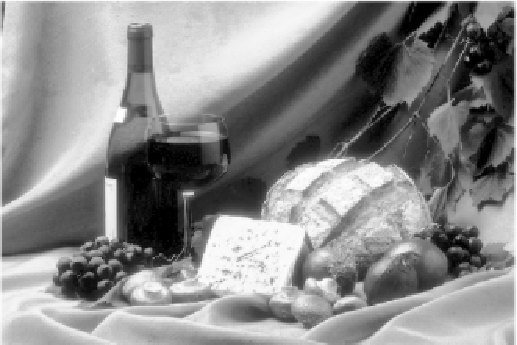
\includegraphics[width=\linewidth]{kennzeichenerkennung/vorBilateral.pdf}
        \caption{Vor Bilateraler Filterung}
        \label{vorBi}
    \end{minipage}
    \hfill
    \begin{minipage}[t]{0.45\linewidth}
        \centering
        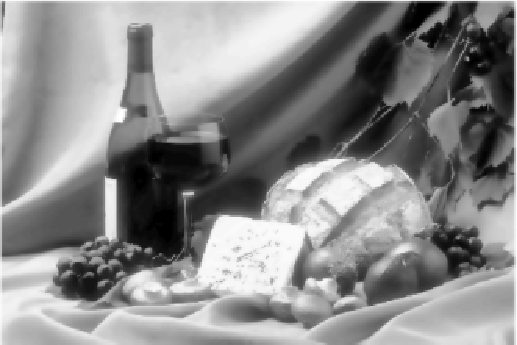
\includegraphics[width=\linewidth]{kennzeichenerkennung/nachBilateral.pdf}
        \caption{Nach Bilateraler Filterung}
        \label{nachBi}
    \end{minipage}
\end{figure}

In Abbildung \ref{vorBi} ist ein Bild mit von verschiedenen Lebensmitteln sehen. Bei genauer Betrachtung sind vor allem bei den Blättern im Hintergrund und beim Brot viele detailreiche Texturen zu erkennen. 
Diese Texturen haben keine wichtige Informationen und sind deswegen unnötig. Um die Bildverarbeitung zu 
vereinfachen wird die bilaterale Filterung auf dieses Bild angewendet, um diese detailreichen 
Texturen zu vereinfachen. In Abbildung \ref{nachBi} ist das Bild nach der bilateralen Filterung zu erkennen. 
Wenn hier dann wieder genauer auf die Blätter und das Brot geachtet wird, ist zu sehen, dass die 
detailreichen Texturen weichgezeichnet wurden, aber die Kanten sind genauso gut erkennbar wie vor der Filterung.

\subsubsection{Thresholding}
Das Thresholding oder auch Schwellenwertverfahren wird in der Bildverarbeitung verwendet, um Bilder zu segmentieren. 
Aus einem Graubild kann dadurch ein Binäres Bild erzeugt werden.\\ 

Bei diesem Verfahren wird ein bestimmter Schwellwert (engl.: Threshold) definiert, welcher mit den Grauwerten der einzelnen 
Pixel des Bildes verglichen wird. Wenn der Grauwert den Schwellwert überschreitet, wird dieser durch einen weißen Pixel 
ersetzt und wenn der Grauwert kleiner als der Schwellwert ist, wird dieser durch einen schwarzen Pixel ersetzt. 
Dadurch erhält man ein Bild welches nur noch zwei Farben hat, Schwarz und Weiß. Dies wird deswegen eingesetzt, 
da dadurch viele Bildverarbeitungsalgorithmen schneller arbeiten und die Effizienz gesteigert wird.\\

\begin{figure}[htbp]
    \centering
    \begin{minipage}[t]{0.45\linewidth}
        \centering
        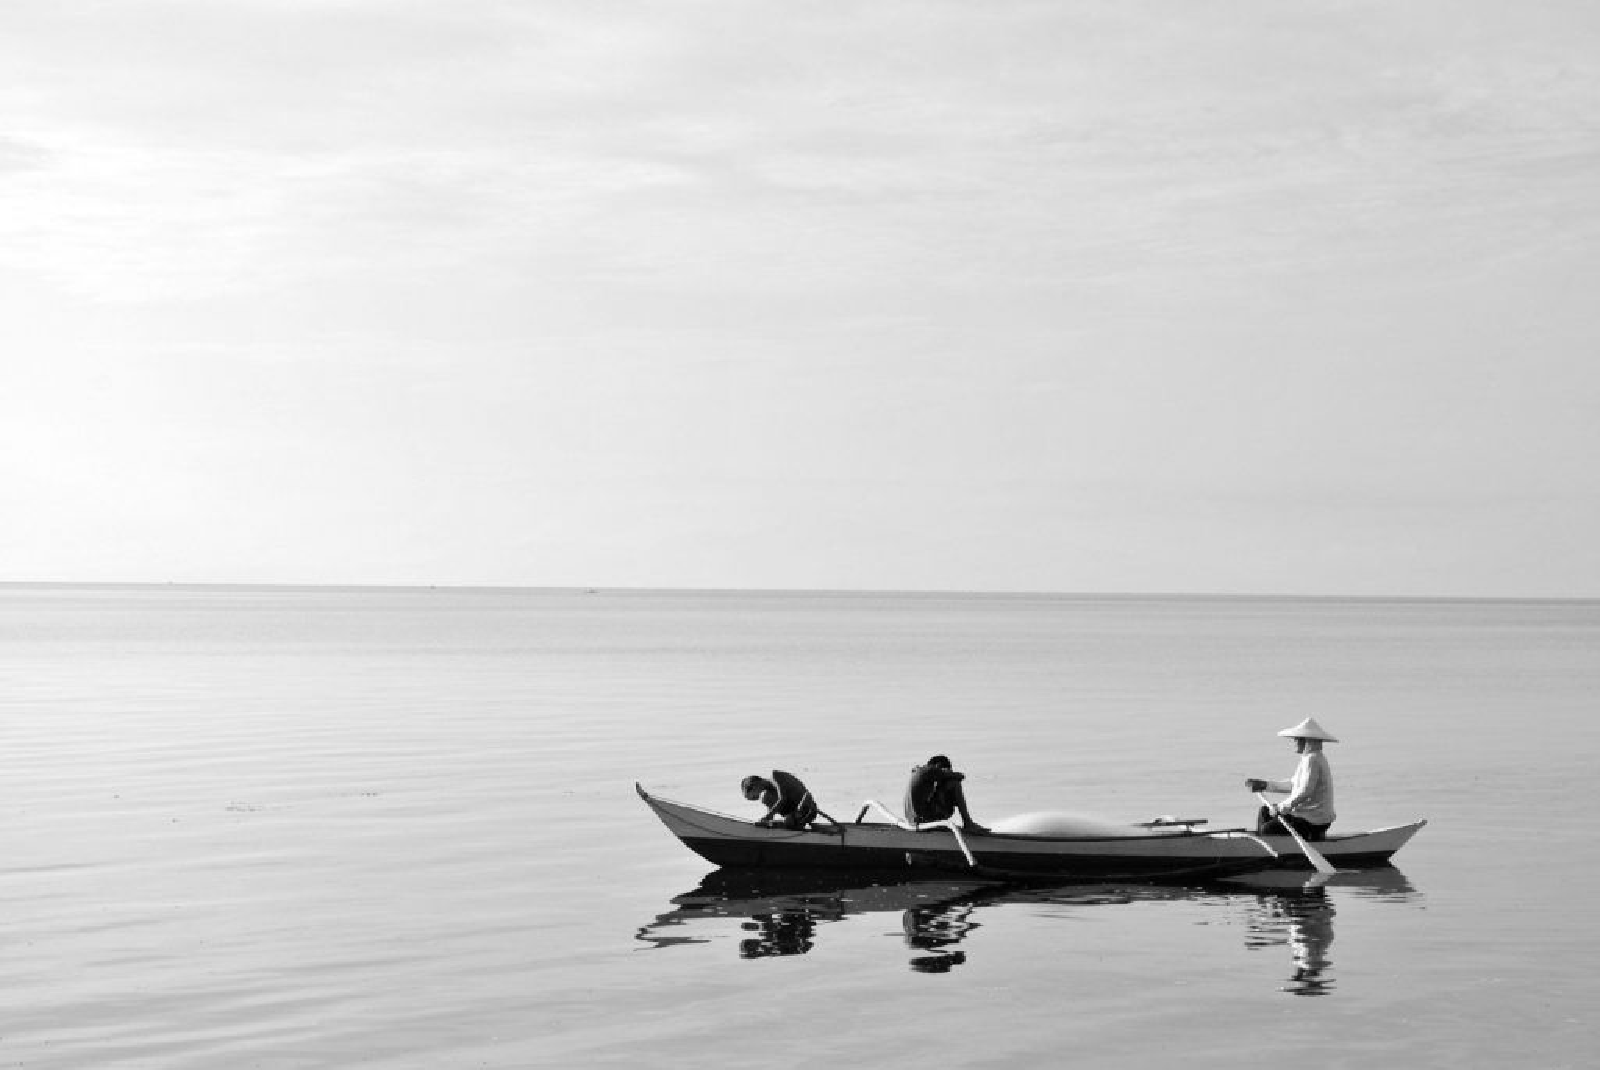
\includegraphics[width=\linewidth]{kennzeichenerkennung/graustufen.pdf}
        \caption{Graustufenbild}
        \label{graypic}
    \end{minipage}
    \hfill
    \begin{minipage}[t]{0.45\linewidth}
        \centering
        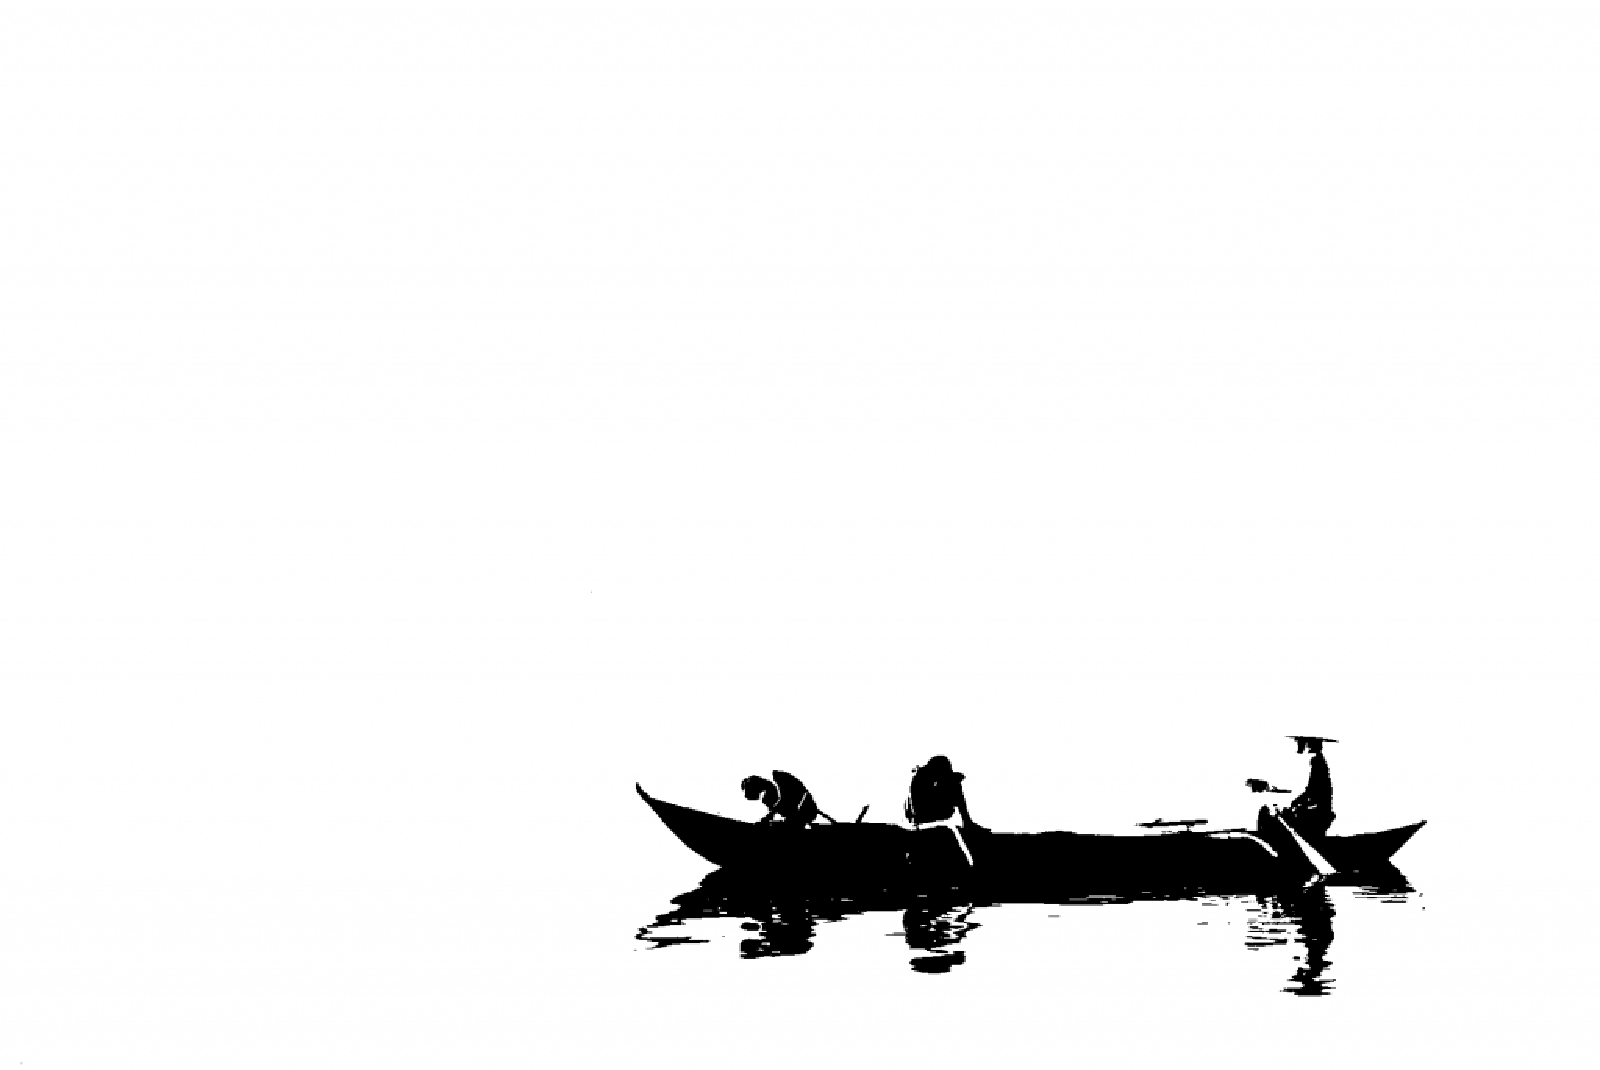
\includegraphics[width=\linewidth]{kennzeichenerkennung/binary.pdf}
        \caption{Binäres Bild nach Thresholding}
        \label{binarypic}
    \end{minipage}
\end{figure}

In Abbildung \ref{graypic} sieht man ein solches Graubild, welches nur verschieden Graustufen aufweist. In Abbildung \ref{binarypic} ist das 
Bild nach dem Thresholding zu erkennen. Hier ist nur noch das Boot mit den Menschen zu erkennen. Dies ist nicht nur für schnellere 
Bildverarbeitungsalgorithmen wichtig, sondern wird auch zur Objekterkennung in Bildern verwendet.\\

Um den Schwellwert zu bestimmen kann man diesen entweder variieren bis das gewünschte Ergebnis erscheint oder man 
verwendet Methoden, welche den Schwellwert automatisch bestimmen. Eine der bekanntesten Methoden zur Schwellwertbestimmung 
ist die Methode von Otsu\footnote{Benannt nach Nobuyuki Otsu}, welche mit dem Schwellenwert die Pixel in Vordergrund und Hintergrund unterteilt.

\subsubsection{Erosion}
Erosion\footnote{\url{https://opencv-python-tutroals.readthedocs.io/en/latest/py_tutorials/py_imgproc/py_morphological_ops/py_morphological_ops.html}} ist eine Funktion der Bildverarbeitung und ist in die morphologische\footnote{Zweig der Bildverarbeitung der sich mit binären Bildern beschäftigt} Bildverarbeitung einzuordnen. Diese beschäftigt 
sich primär mit der Verarbeitung von binären Bildern, welche man nach Thresholding erhält. Das Ziel der Erosion ist es dabei Störungen zu verringern.\\

Erosion benötigt zwei Eingaben, das binäre Bild und einen Kernel. Der Kernel ist dabei die Angabe, nach welcher die Erosion 
durchgeführt wird. Der Kernel ist auch eine binäre Struktur, welche über jeden einzelnen Pixel des binären Bildes geschoben 
wird. Wenn der Kernel komplett mit dem binären Bild übereinstimmt, behält dieser Pixel seinen Wert und ansonsten wird er 
invertiert. Dabei muss jedoch darauf geachtet werden, dass die Polarität des binären Bildes und des Kernels übereinstimmt, 
da sonst die Erosion nicht richtig funktioniert. Als Resultat erhält man danach ein deutlicheres Bild bei welchem einzelne 
Pixelfehler herausgefiltert wurden und die Konturen besser erkennbar sind.\\

\begin{figure}[htbp]
    \centering
    \begin{minipage}[t]{0.45\linewidth}
        \centering
        
\includegraphics[width=\linewidth]{kennzeichenerkennung/kennBinary.pdf}
        \caption{Binäres Bild nach Thresholding}
        \label{kennbinpic}
    \end{minipage}
    \hfill
    \begin{minipage}[t]{0.45\linewidth}
        \centering
        
\includegraphics[width=\linewidth]{kennzeichenerkennung/kennErosion.pdf}
        \caption{Nach Erosion}
        \label{eropic}
    \end{minipage}
\end{figure}

In Abbildung \ref{kennbinpic} und \ref{eropic} sieht man die Anwendung der Erosion. Die Konturen der einzelnen Zeichen im Kennzeichen sind in Abbildung 
\ref{eropic} nach der Erosion deutlicher erkennbar als davor.

\subsubsection{Farbraum}
Der Farbraum eines Bildes enthält alle möglichen Farben eines Farbmodells. Das Farbmodell beschreibt dabei die Parameter, aus 
welchen die einzelnen Farben gebildet werden. Dies ist in der Bildverarbeitung relevant, da verschiedene Funktionen der 
Bildverarbeitung, unterschiedliche Farbräume verwenden und dieser deswegen korrekt eingestellt werden muss.\\

In dieser spezifischen Applikation werden die folgenden Farbräume verwendet:

\paragraph{RGB}\mbox{}\\
RGB ist einer der häufigsten und bekanntesten Farbräume. Er basiert auf den drei Grundfarben Rot, Grün und Blau und wird vor 
allem bei Bildschirmen und in der Fotografie genutzt. Die Farben setzen sich in diesem Modell aus dem jeweiligen Rot-, Grün- 
und Blauanteil der einzelnen Pixel zusammen.

\paragraph{Graustufen}\mbox{}\\
Bei einem Graustufen-Bild, zu sehen in Abbildung 3, hat jeder Pixel einen Wert von 0 bis 255. Diese Werte erstrecken sich also 
von Schwarz bis Weiß und dazwischen liegen verschiedene Grautöne. Dieser Farbraum wird in der Bildverarbeitung häufig verwendet, 
da Konturen einfacher erkennbar sind und es nur einen Parameter gibt, welcher verarbeitet werden muss, wodurch die Effizienz 
diverser Algorithmen gesteigert werden kann. Zudem wird dieser Farbraum auch oft in Verbindung mit Thresholding verwendet.

\paragraph{BGR}\mbox{}\\
Der BGR ist ein relativ unbekannter und wenig verwendeter Farbraum, da er sehr ähnlich zum RGB-Farbraum ist. Der einzige 
Unterschied zwischen diesen beiden liegt in der Anordnung der Parameter. Bei BGR sind die Parameter spiegelverkehrt zu RGB, 
das heißt es kommt zuerst der Blauanteil, dann der Grünanteil und zum Schluss der Rotanteil. Insgesamt ergibt dies für die 
einzelnen Pixel zwar die gleichen Farben, aber die Funktionen der Bildverarbeitung müssen trotzdem das Bild im passenden 
Farbraum erhalten. So verwendet zum Beispiel die Funktion „imread“ von OpenCV den BGR-Farbraum und die Funktion „imShow“ 
von Matplotlib verwendet den RGB-Farbraum. Wenn man diese Funktionen also nacheinander anwendet, muss dazwischen der Farbraum 
umgewandelt werden.

\subsubsection{Konturerkennung}
Die Konturerkennung ist eine wichtige Funktion in der Bildverarbeitung mit welcher Objekte in einem Bild gefunden werden können. 
In dieser Applikation wird sie für die Zeichensegmentierung eingesetzt.\\

Die Konturerkennung wird hauptsächlich bei binären Bildern verwendet. Eine Kontur kann dabei wie im Folgenden definiert werden. 
Man überprüft jeden einzelnen Pixel und sieht nach, ob ein benachbarter Pixel einen anderen Farbwert aufweist. Falls dies 
zutrifft muss der zu prüfende Pixel zu einer Kontur gehören. Wenn dies auf mehrere zusammenhängende Pixel zutrifft, bedeutet 
das, dass diese zusammen eine Kontur bilden.\\

Die Funktion „findcontours“ von OpenCV, welche in dieser Applikation verwendet wird, ist eine Funktion für Konturerkennung 
und kann weiße Objekte auf einem schwarzen Hintergrund erkennen. Sie basiert auf dem Algorithmus von Suzuki von 
1985\footnote{Topological structural analysis of digitized binary images by border following} und 
liefert eine Liste mit allen Konturen. Die Konturen werden in der Liste als ein Array von Koordinaten abgespeichert.

\subsection{Kennzeichenerkennungsprogramm}

\subsubsection{Einleitung}
Die Software ist der wichtigste und größte Teil der Kennzeichenerkennung. Sie erhält ein Bild, in welchem ein Auto mit 
einem Kennzeichen enthalten ist und liefert am Ende dieses Kennzeichen und sendet dieses dann automatisch an die Datenbank. 
Die Software kann entweder über Bildverarbeitung oder mit Modellen für maschinelles Lernen realisiert werden. Der erste Ansatz bei 
dieser Anwendung war mit klassischer Bildverarbeitung, welche aber nicht die gewünschte Genauigkeit erreicht hat, weswegen 
dann auf maschinelles Lernen gewechselt wurde.

\subsubsection{Programmiersprache}
Die verwendete Programmiersprache für die Kennzeichenerkennung ist Python\footnote{\url{https://www.python.org/}}. Python ist eine höhere Programmiersprache, 
welche übersichtlich und leicht lesbar ist. Sie ist vor allem für Bildverarbeitung und Anwendungen mit maschinellem Lernen gut geeignet, 
da es dafür hoch optimierte und effiziente Bibliotheken gibt wie zum Beispiel OpenCV\footnote{\url{https://opencv.org/}}, Numpy\footnote{\url{https://numpy.org/}} und Tensorflow\footnote{\url{https://www.tensorflow.org/}}. Dadurch ist Python 
für diese Anwendung besser geeignet als zum Beispiel C++. Dieses wäre zwar normalerweise effizienter, bietet aber weniger 
optimierte Bibliotheken in diesem Bereich, wodurch es hier weniger gut geeignet ist.

\subsubsection{Konzept}
Das Programm für die Kennzeichenerkennung basiert auf fünf Stufen. Die erste Stufe ist die Bildaufnahme, die zweite ist die 
Kennzeichenerfassung mittels maschinellem Lernen, die dritte ist die Kennzeichensegmentierung mithilfe von Bildverarbeitung, 
die vierte ist die Zeichenerkennung mittels maschinellem Lernen und die fünfte ist die Anbindung an die Datenbank.

\paragraph{Bildaufnahme}\mbox{}\\
Um ein Bild verarbeiten zu können und aus diesem ein Kennzeichen auszulesen, muss zuerst ein Bild vorliegen. 
Dieses wird über den Raspberry Pi mit der Raspberry Pi-Kamera aufgenommen. Um das Bild aufzunehmen, muss einfach ein Auslöser 
aktiviert werden und dann wird das Bild aufgenommen und im richtigen Ordner abgespeichert. Zuvor wird noch überprüft ob 
sich in diesem Ordner bereits ein Bild befindet und falls eines vorhanden ist wird es gelöscht. Dadurch werden mögliche Fehler 
durch mehrere Bilder verhindert.

\paragraph{Kennzeichenerfassung}\mbox{}\\
Die Kennzeichenerfassung hat die Aufgabe, das Kennzeichen im Eingabebild zu lokalisieren. Dies geschieht mittels maschinellem Lernen 
mit dem Modul WPOD-NET von Sérgio Montazolli Silva und Cláudio Rosita Jung\footnote{\cite{wpodnet}}. Dieses verwendet zuerst das Modul YOLOv2\footnote{\cite{YOLO9000}} welches zur 
Echtzeitobjekterkennung verwendet werden kann und in dieser Anwendung zur Erkennung von Fahrzeugen verwendet wird. Danach werden 
die Koordinaten des Kennzeichens ermittelt und dieses aus dem Bild ausgeschnitten und abgespeichert.

\paragraph{Kennzeichensegmentierung}\mbox{}\\
Die Kennzeichensegmentierung hat das Ziel die einzelnen Zeichen im Kennzeichen zu separieren und so vorzubereiten, dass die 
darauffolgende Zeichenerkennung damit arbeiten kann. Dazu wird das Bild mit dem Kennzeichen zuerst in Graustufen konvertiert, 
dann mit einem bilateralen Filter gefiltert, mit Thresholding in ein binäres Bild umgewandelt und anschließend mittels Erosion verarbeitet, damit es besser erkennbar ist. Danach werden im verarbeiteten Bild die Konturen gesucht, sortiert und anhand dieser die einzelnen Zeichen herausgefiltert.

\paragraph{Zeichenerkennung}\mbox{}\\
Die letzte Stufe der Kennzeichenerkennung ist die Zeichenerkennung. In dieser werden die einzelnen Zeichen erkannt und als Text 
abgespeichert. Dies funktioniert über ein eigenes neuronales Netz basierend auf MobileNetV2\footnote{neuronales Netz für Computer Vision}, welches mit einem Datensatz von 
über 35 000 Bildern auf die Erkennung von Zeichen aus Bildern trainiert wurde.

\paragraph{Anbindung an Datenbank}\mbox{}\\
Nachdem das Kennzeichen als Text abgespeichert wurde, muss diese Information in die Datenbank übergeben werden. Dazu wird die 
eigene API verwendet, welcher man diese Informationen übergeben muss und als Rückgabe die Information bekommt, ob sich das 
Fahrzeug nun innerhalb oder außerhalb des Parkplatzes befindet.

\subsubsection{Ablauf}

\begin{figure}[H]
    \centering
    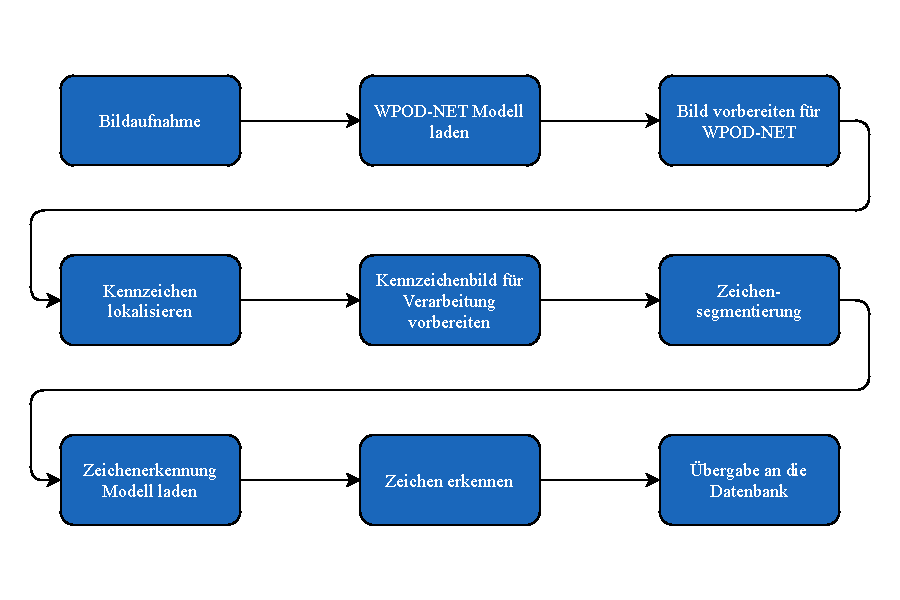
\includegraphics[width=0.9\linewidth]{kennzeichenerkennung/Programmablauf.pdf}
    \caption{Ablaufdiagramm der Kennzeichenerkennung}
\end{figure}

Im oberen Diagramm ist der Ablauf des Programms angegeben. Zuerst wird mit einem Button der Auslöser betätigt und damit das 
Foto aufgenommen. Dann wird das erste Modell für maschinelles Lernen für die Kennzeichenerkennung „WPOD-NET“\footnote{Modell für maschinelles Lernen für Kennzeichenerfassung} geladen. Bevor das 
Bild diesem Modell übergeben werden kann, muss es noch angepasst werden, damit das Modell damit arbeiten kann. Danach kann 
damit das Kennzeichen im Bild lokalisiert werden. Im Anschluss wird dieses Kennzeichenbild mit mehreren Bildverarbeitungsalgorithmen 
verarbeitet, um dann die einzelnen Zeichen zu segmentieren. Danach kann dann das Modell für die Zeichenerkennung geladen 
werden und dieses dann auch angewendet werden, um das Ergebnis zu erhalten. Dieses Ergebnis wird dann noch mit einer API an die Datenbank übergeben.

\subsubsection{Verwendete Libraries}

\paragraph{Versionsübersicht der verwendeten Libraries}\mbox{}\\
Im Folgenden werden die verwendeten Versionen der benötigten Libraries aufgelistet, um das Programm zu starten. Dies wird noch einmal 
unterteilt in die Versionen, welche auf Windows 10 benötigt werden und jene auf Raspbian\footnote{Raspbian ist ein Unix-basiertes Betriebssystem für den Raspberry Pi}, da auf Raspbian manche Versionen noch 
nicht verfügbar sind, neuere und verbesserte Versionen verfügbar sind oder manche Versionen nur auf komplizierten Umwegen installierbar sind.

\begin{figure}[htbp]
    \centering
    \begin{minipage}[t]{0.45\linewidth}
        Windows:
        \begin{itemize}
            \item h5py = 2.10.0
            \item imutils = 0.5.3
            \item Keras = 2.4.3
            \item matplotlib = 3.3.2
            \item notebook = 6.1.5
            \item numpy = 1.18.5
            \item opencv-python = 4.4.0.44
            \item scikit-learn = 0.23.2
            \item tensorflow = 2.3.1
            \item requests = 2.24.0
        \end{itemize}
    \end{minipage}
    \hfill
    \begin{minipage}[t]{0.45\linewidth}
        Raspbian:
        \begin{itemize}
            \item h5py = 2.10.0
            \item imutils = 0.5.3
            \item Keras = 2.4.3
            \item matplotlib = 3.3.3
            \item notebook = 6.1.5
            \item numpy = 1.19.4
            \item opencv-python = 4.4.0.46
            \item scikit-learn = 0.24.0
            \item tensorflow = 2.4.0
            \item requests = 2.21.0
        \end{itemize}
    \end{minipage}
\end{figure}

In der oberen Tabelle sind die benötigten Versionen der Libraries aufgelistet. Dabei wird jene Bezeichnung verwendet, mit welcher die Library in Python angesprochen wird.

\paragraph{Jupyter Notebook}\mbox{}\\
Jupyter Notebook\footnote{\url{https://jupyter.org/}} ist eine nützliche Erweiterung für Python, wenn es um den Bereich der Daten-Visualisierung und maschinelles Lernen geht. 
Sie ist eine Unteranwendung des Open-Source Projektes „Project Jupyter“, welches von großen Partnern wie Microsoft und Google unterstützt 
und verwendet wird. Mit Jupyter Notebook ist es möglich in einer Web-Anwendung ein Live-Script abzuarbeiten und in Kombination mit Matplotlib 
die Daten visuell darzustellen, abzuspeichern und zu überwachen. Im Gegensatz zur direkten Darstellung in der Entwicklungsumgebung, wird 
der letzte Durchgang des Scripts, inklusive aller Bilder und Grafiken, gespeichert. Zudem ist es auch hervorragend für das Training und 
die dazugehörende Überwachung von Modulen für maschinelles Lernen geeignet. Außerdem bietet Jupyter Notebook noch die Möglichkeit mehrere Scripts 
parallel abzuarbeiten und diese individuell zu überwachen. In dieser Applikation wird es für ein solches Training und für die anschauliche 
Visualisierung von Daten genutzt.\\

Die Installation von Jupyter Notebook ist simpel, da man es einfach über pip\footnote{Paketverwaltungsprogramm für Python} mit dem folgenden Befehl installieren kann:

\begin{listing}[H]
    \begin{minted}{bash}
    pip install notebook
    \end{minted}
    \caption{PIP Installation von Jupyter Notebook}
\end{listing}

Um das Jupyter Notebook aufzurufen muss im Terminal „jupyter notebook“ eingegeben werden und dann öffnet sich automatisch die Web-Applikation. 
Danach hat man Zugriff auf die komplette Dateistruktur des eigenen Projektes und kann die einzelnen Python-Scripts starten. Dabei ist zu beachten, 
dass man keine gewöhnliche \verb|.py|-Datei benötigt, sondern eine \verb|.ipynb|-Datei benötigt, wozu man einfach eine Kopie des normalen Scripts erstellt und die Dateiendung ändert.

\paragraph{Numpy}\mbox{}\\
Numpy ist eine weit verbreitete Library für Python, welche sich mit der Berechnung und Verarbeitung von mehrdimensionalen Arrays beschäftigt. 
Damit können komplexe Berechnungen und Algorithmen oft effizienter verarbeitet werden, wobei aber beachtet werden muss, dass der Code an die 
mehrdimensionalen Arrays angepasst werden muss. Numpy selbst ist auch eine Voraussetzung für OpenCV, welches Numpy-Arrays verwendet, um Bilder zu verarbeiten. 
Dazu werden 3-dimensionale Arrays verwendet, wodurch die Verarbeitung dieser Bilder und die Bildverarbeitungsalgorithmen schneller sind. In dieser 
Applikation wird Numpy in Zusammenarbeit mit OpenCV verwendet und auch für die weitere Verarbeitung der Daten von OpenCV, um zum Beispiel die 
Koordinaten des Kennzeichens zu speichern.\\

Um Numpy zu installieren muss folgender Befehl in der Kommandozeile eingegeben werden:

\begin{listing}[H]
    \begin{minted}{bash}
    pip install numpy
    \end{minted}
    \caption{PIP Installation von Numpy}
\end{listing}

\paragraph{OpenCV}\mbox{}\\
OpenCV ist die wichtigste und mächtigste Library die in dieser Applikation verwendet wird. Sie wurde ursprünglich in C++ geschrieben, 
aber es gibt auch eine Version in Python, welche in dieser Applikation verwendet wird. OpenCV ist eine freie Library für Bildverarbeitung, 
Computer Vision\footnote{Die Computergestütze Auswertung und Verarbeitung von Kamerabildern} und maschinelles Lernen, welche von Intel gestartet wurde und mittlerweile die wichtigste und am weitesten verbreitete 
Library in diesem Bereich ist. Sie verwendet Numpy-Arrays, um für eine effiziente Verarbeitung von Bildern zu sorgen. Einige der wichtigsten 
Funktionen stellen die klassischen Bildverarbeitungsalgorithmen wie zum Beispiel Filterung und Farbraumanpassungen, die Verarbeitung und 
Auswertung von Kamerabildern und auch die Kompatibilität mit Deep-Learning\footnote{Methode für maschinelles Lernen welche neuronale Netze nutzt} dar. In dieser Applikation wird OpenCV für diverse 
Bildverarbeitungsalgorithmen, die Zusammenarbeit mit Modellen für maschinelles Lernen, die Verarbeitung eines Kamerabildes und das allgemeine Arbeiten mit Bildern verwendet.\\

Die Installation von OpenCV ist dabei etwas komplizierter als bei anderen Libraries.\\

Windows:\\

Unter Windows ist die Installation vergleichbar mit anderen Libraries, es muss einfach der folgende Befehl in der Kommandozeile eingegeben werden:

\begin{listing}[H]
    \begin{minted}{bash}
    pip install opencv-python
    \end{minted}
    \caption{PIP Installation von OpenCV}
\end{listing}

Raspbian:\\

Auf dem Raspberry Pi gestaltet sich die Installation von OpenCV um einiges schwieriger, da die Installation nicht über pip ausgeführt werden kann, 
sondern es manuell kompiliert werden muss.\\

Als erstes werden alle Tools und Bibliotheken installiert, welche für OpenCV benötigt werden. Dazu verwendet man folgenden Befehl im Terminal:

\begin{listing}[H]
    \begin{minted}{bash}
    $ sudo apt-get install build-essential git cmake pkg-config libjpeg8-dev libtiff4-dev libjasper-dev libpng12-dev libavcodec-dev libavformat-dev libswscale-dev libv4l-dev libgtk2.0-dev libatlas-base-dev gfortran
    \end{minted}
    \caption{Installation benötigter Tools und Bibliotheken für OpenCV}
\end{listing}

Danach kann man mit dem nächsten Befehl OpenCV von einem GitHub-Repository klonen:

\begin{listing}[H]
    \begin{minted}{bash}
    $ sudo apt-get install build-essential git cmake pkg-config libjpeg8-dev libtiff4-dev libjasper-dev libpng12-dev libavcodec-dev libavformat-dev libswscale-dev libv4l-dev libgtk2.0-dev libatlas-base-dev gfortran
    \end{minted}
    \caption{Klonen von OpenCV von GitHub}
\end{listing}

Im nächsten Schritt wird OpenCV mit den folgenden Befehlen kompiliert:

\begin{listing}[H]
    \begin{minted}{bash}
    cd ~/opencv && mkdir build && cd build

    cmake -D CMAKE_BUILD_TYPE=RELEASE \
    -D CMAKE_INSTALL_PREFIX=/usr/local \
    -D INSTALL_PYTHON_EXAMPLES=ON \
    -D INSTALL_C_EXAMPLES=ON \
    -D OPENCV_EXTRA_MODULES_PATH=~/opencv_contrib/modules \
    -D BUILD_EXAMPLES=ON ..
    make -j4
    \end{minted}
    \caption{Kompilieren von OpenCV}
\end{listing}

Wenn das Kompilieren erfolgreich beendet wurde, kann OpenCV abschließend installiert werden.

\begin{listing}[H]
    \begin{minted}{bash}
    $ sudo make install && sudo ldconfig
    \end{minted}
    \caption{Abschließende Installation von OpenCV}
\end{listing}

Danach sollte OpenCV fertig installiert und eingerichtet sein und es kann in einem Python Projekt verwendet werden.

\paragraph{Matplotlib}\mbox{}\\
Matplotlib\footnote{\url{https://matplotlib.org/}} ist eine Python-Library mit welcher Daten und Berechnungen visuell dargestellt werden können. Damit können 
statische, animierte und interaktive Diagramme erstellt werden, was die Datenauswertung um einiges erleichtert. 
Die Syntax ähnelt sehr stark jener von MATLAB, wodurch die Bedienung sehr einfach ist, wenn man schon Erfahrung mit 
MATLAB hat. Wie auch in MATLAB kann man die Diagramme beliebig anordnen und dadurch das Layout der Darstellung selbst 
festlegen. Es funktioniert auch hervorragend in Zusammenarbeit mit Jupyter Notebook, wodurch man die Daten in einer 
Web-Applikation visualisieren kann. Die visuelle Darstellung von Daten ist vor allem in der Entwicklung und beim 
Arbeiten mit visuellen Ergebnissen wie Bildern von Vorteil. In dieser Applikation wird Matplotlib für die Darstellung 
der Ergebnisse von Bildverarbeitungsalgorithmen, die Ausgabe von Daten und Resultaten und auch für Test- und 
Entwicklungszwecke verwendet. Im unteren Bild kann man ein Beispiel sehen bei welchem Matplotlib verwendet wird, 
um einige Bilder mit einem Titel anzuzeigen.

\begin{figure}[H]
    \centering
    
\includegraphics[width=0.9\linewidth]{kennzeichenerkennung/matplotlibbsp.pdf}
    \caption{Beispiel einer Anwendung von Matplotlib}
\end{figure}

Um Matplotlib zu installieren muss das Folgende in der Kommandozeile eingegeben werden:

\begin{listing}[H]
    \begin{minted}{bash}
    pip install matplotlib
    \end{minted}
    \caption{PIP Installation von Matplotlib}
\end{listing}

\paragraph{Keras}\mbox{}\\
Keras\footnote{\url{https://keras.io/}} ist eine Deep-Learning Schnittstelle für diverse Machine Learning Frameworks wie zum Beispiel Tensorflow oder Theanos. 
Damit wird die Bedienung und Anwendung dieser Frameworks vereinfacht und es bietet auch diverse Funktionen, um die Kompatibilität der Inputs mit 
den Modellen für maschinelles Lernen zu ermöglichen. Keras ist ein Teil von Tensorflow, wird aber eigenständig weiterentwickelt, 
um die Kompatibilität mit anderen Machine Learning Frameworks aufrechtzuerhalten. In dieser Applikation wird es in 
Zusammenarbeit mit Tensorflow verwendet, um mit den verwendeten Modellen für maschinelles Lernen zu arbeiten.\\

Um Keras zu installieren führt man folgenden Befehl in der Kommandozeile aus:

\begin{listing}[H]
    \begin{minted}{bash}
    pip install keras
    \end{minted}
    \caption{PIP Installation von Keras}
\end{listing}

\paragraph{Tensorflow}\mbox{}\\
Tensorflow ist eines der weltweit beliebtesten Frameworks für maschinelles Lernen und wird von weltweit erfolgreichen Firmen wie 
zum Beispiel Google, AMD oder auch Intel verwendet. Es bietet eine umfassende Plattform für jegliche Anwendungen für maschinelles Lernen 
und ist in Zusammenarbeit mit APIs wie zum Beispiel Keras leicht zu verwenden. In dieser Applikation wird damit ein neuronales 
Netz trainiert und mehrere Modelle für maschinelles Lernen verwaltet und verwendet.\\

Bei der Installation von Tensorflow muss beachtet werden, dass sich diese von Windows zu Raspbian stark unterscheidet. 
Raspbian unterstützt offiziell die benötigte Version von Tensorflow noch nicht und deswegen muss dieses über ein paar Umwege installiert werden.\\

Windows:\\

Die Installation von Tensorflow unter Windows ist einfach, da man es wie andere Libraries einfach über pip installieren kann.

\begin{listing}[H]
    \begin{minted}{bash}
    pip install tensorflow
    \end{minted}
    \caption{PIP Installation von Tensorflow}
\end{listing}

Raspbian:\\

Bei Raspbian muss Tensorflow manuell kompiliert werden, da die aktuelle Version noch nicht offiziell unterstützt wird. Diese funktioniert 
aber trotz dieses Umweges einwandfrei und wird mit den folgenden Befehlen in der Kommandozeile installiert.\\

Mit dem ersten Befehl werden die benötigten Tools installiert:

\begin{listing}[H]
    \begin{minted}{bash}
    $ sudo apt-get install cmake curl
    \end{minted}
    \caption{Benötigte Tools für Tensorflow}
\end{listing}

Danach kann man die neuste Tensorflow Version von GitHub herunterladen:

\begin{listing}[H]
    \begin{minted}{bash}
    $ wget -O tensorflow.zip https://github.com/tensorflow/tensorflow/archive/v2.4.0.zip
    \end{minted}
    \caption{Tensorflow von GitHub herunterladen}
\end{listing}

Anschließend muss Tensorflow entpackt werden:

\begin{listing}[H]
    \begin{minted}{bash}
    $ unzip tensorflow.zip
    $ mv tensorflow-2.4.0 tensorflow
    $ cd tensorflow
    \end{minted}
    \caption{Entpacken von Tensorflow}
\end{listing}

Im nächsten Schritt müssen noch zusätzlich erforderliche Libraries installiert werden:

\begin{listing}[H]
    \begin{minted}{bash}
    $ ./tensorflow/lite/tools/make/download_dependencies.sh
    \end{minted}
    \caption{Zusätzlich erforderliche Libraries}
\end{listing}

Danach kann die Installation kompiliert werden:

\begin{listing}[H]
    \begin{minted}{bash}
    $ ./tensorflow/lite/tools/make/build_aarch32_lib.sh
    \end{minted}
    \caption{Kompilieren von Tensorflow}
\end{listing}

Danach muss man die Installation mit den folgenden Befehlen abschließen:

\begin{listing}[H]
    \begin{minted}{bash}
    $ cd ~/tensorflow/tensorflow/lite/tools/make/downloads/flatbuffers
    $ mkdir build
    $ cd build
    $ cmake ..
    $ make -j4
    $ sudo make install
    $ sudo ldconfig
    \end{minted}
    \caption{Abschließen der Installation von Tensorflow}
\end{listing}

Nach diesem Schritt sollte die Tensorflow Installation funktionieren und man kann es wie jede andere Library in Python einbinden.

\paragraph{local{\_}utils}\mbox{}\\
local{\_}utils ist ein einfaches Python-Script, welches die Arbeit mit WPOD-NET im Bereich der Kennzeichenerkennung vereinfacht. Es beinhaltet die Funktion „detect{\_}lp“ mit 
welcher ein Bild des Kennzeichens und die Koordinaten des Kennzeichens ermittelt werden können. Dieses Script kann über den 
folgenden Link von GitHub heruntergeladen werden: \url{https://github.com/quangnhat185/Plate_detect_and_recognize/blob/master/local_utils.py} 

\paragraph{Scikit-learn}\mbox{}\\
Scikit-learn\footnote{\url{https://scikit-learn.org/stable/}} ist eine freie Library für maschinelles Lernen und basiert auf Numpy und Matplotlib. Es wird vor allem verwendet, 
um mit großen visuellen Datensätzen neuronale Netze zu trainieren.  Es bietet Funktionen, um Modelle anzupassen, Daten vorzubereiten, 
Modelle zu trainieren und ähnliches. In dieser Applikation wird es für die Normalisierung von Labels verwendet, um diese für Modelle für maschinelles Lernen anzupassen und für das zufällige Aufteilen von Arrays in Test und Trainingsteile, welche für das Training eines neuronalen Netzes benötigt werden.\\

Für die Installation von Scikit-learn muss die folgende Zeile in der Kommandozeile ausgeführt werden:

\begin{listing}[H]
    \begin{minted}{bash}
    pip install scikit-learn
    \end{minted}
    \caption{PIP Installation von Scikit-learn}
\end{listing}

\paragraph{Requests}\mbox{}\\
Requests ist eine Library mit welcher HTTP-Anfragen in Python vereinfacht werden. Sie wird häufig verwendet, um mit APIs zu kommunizieren 
und ist eine der beliebtesten Python Libraries, da sie für API-Anwendungen so gut wie notwendig ist. In dieser Applikation wird sie für die 
Kommunikation zu einer eigenen API für den Datenbankzugriff verwendet. Dadurch ist es ohne größere Schwierigkeiten möglich, das Bild des Kennzeichens, 
die ID für den jeweiligen Parkplatz und das Resultat des Kennzeichens an die eigene Datenbank zu senden und auch eine Antwort zu erhalten, ob der 
Zugriff erfolgreich war. Um die Daten mit dieser Library zu übertragen müssen diese einfach nur in einem Dictionary eingetragen werden und dann mit 
dem korrekten Schlüsselwort über die API gesendet werden.\\

Die Installation von Requests erfolgt mit folgendem Befehl in der Kommandozeile:

\begin{listing}[H]
    \begin{minted}{bash}
    pip install requests
    \end{minted}
    \caption{PIP Installation von Requests}
\end{listing}

\paragraph{Gpiozero}\mbox{}\\
Gpiozero ist eine Python-Library für den Raspberry Pi. Mit ihr ist es möglich auf die GPIO-Pins des Raspberry zuzugreifen, Signale von diesen 
auszulesen und Signale an diesen auszugeben. Dies wird oft verwendet, um Sensoren auszuwerten oder um Aktoren zu steuern, da diese Pins frei 
programmierbar sind, wodurch man jede beliebige Anwendung realisieren kann. Der Raspberry Pi kann zwar keine größeren Aktoren wie zum Beispiel einen Motor direkt ansteuern, 
dies kann aber zum Beispiel mit einem Relais umgangen werden, wodurch der Raspberry Pi zu einem mächtigen Werkzeug für die Sensorik und Aktorik wird. 
Ein Beispiel für die möglichen Anwendungen ist ein Button oder eine Lampe. In dieser Applikation wird mit dieser Library ein gedrückter Button detektiert, 
welcher als Auslöser für die Kamera fungiert.\\

In der folgenden Abbildung sieht man ein Bild der GPIO-Pins des Raspberry Pi, welche mit dieser Library angesteuert werden können:

\begin{figure}[H]
    \centering
    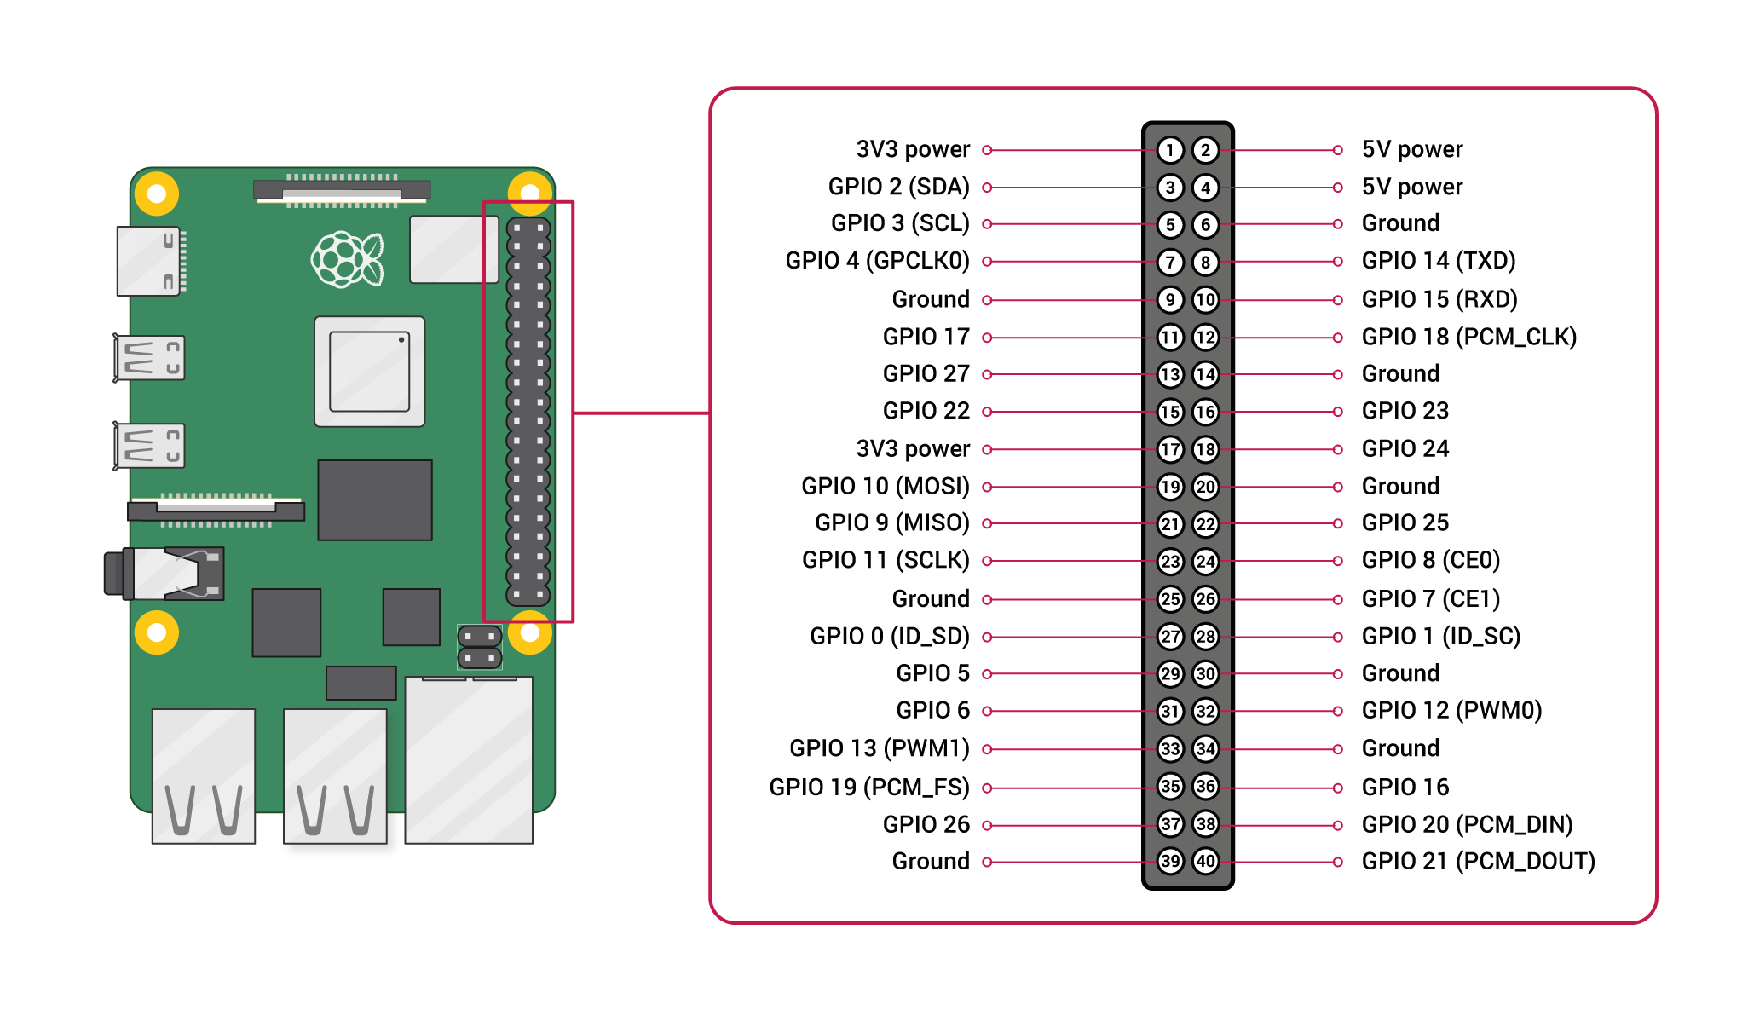
\includegraphics[width=0.8\linewidth]{kennzeichenerkennung/GPIO-Pinout-Diagramm-2.pdf}
    \caption{GPIO-Pins des Raspberry Pi \url{https://www.raspberrypi.org/documentation/usage/gpio/}}
\end{figure}

Diese Library kann nur auf dem Raspberry Pi installiert werden. Um die Library Gpiozero zu installieren kann pip verwendet werden:

\begin{listing}[H]
    \begin{minted}{bash}
    pip install gpiozero
    \end{minted}
    \caption{PIP Installation von Gpiozero}
\end{listing}

\paragraph{Picamera}\mbox{}\\
Die Library picamera wird verwendet, um auf das Kameramodul des Raspberry Pi zuzugreifen. Die Library bietet etliche Funktionen an, 
mit welchen die Kamera gesteuert werden kann, wie zum Beispiel Fotos aufnehmen, Videoaufnahmen zu starten und zu beenden, Fotoeinstellungen 
zu ändern und ähnliches. Die Library ist notwendig, wenn man über Python das Kameramodul bedienen will. In dieser Applikation wird sie verwendet, 
um ein Vorschaubild des aufgenommenen Bildes auf dem Bildschirm darzustellen, falls ein Bildschirm angeschlossen wird und um im 
Anschluss das Bild aufzunehmen und korrekt zu skalieren.\\

Die Installation von picamera ist nur auf dem Raspberry Pi möglich, da nur dieser damit arbeiten kann. 
Für die Installation von picamera muss folgender Befehl in der Kommandozeile eingegeben werden:

\begin{listing}[H]
    \begin{minted}{bash}
    pip install picamera
    \end{minted}
    \caption{PIP Installation von Picamera}
\end{listing}

\subsubsection{Wichtige Programmteile}

Im folgenden Abschnitt werden die wichtigsten Teile des Kennzeichenerkennungsprogrammes genauer betrachtet und erklärt.

\paragraph{WPOD-NET-Modell laden}\mbox{}\\

\begin{listing}[H]
    \begin{minted}{python}
    def load_model(path):
    try:
        path = splitext(path)[0]
        with open ('%s.json' % path, 'r') as json_file:
            model_json = json_file.read()
        model = model_from_json(model_json, custom_objects={})
        model.load_weights('%s.h5' % path)
        print("-> Model loading finished")
        return model
    except Exception as e:
        print(e)
    \end{minted}
    \caption{WPOD-NET Modell laden}
\end{listing}

Für das Lokalisieren des Kennzeichens wird das Model für maschinelles Lernen WPOD-NET verwendet. Dieses basiert auf YOLOv2, 
mit welchem eine Echtzeitobjekterkennung möglich ist und wurde für diese Anwendung so angepasst, dass es möglich ist 
Kennzeichen in einem Bild zu lokalisieren. WPOD-NET versucht zuerst auf Grundlage von YOLOv2 in dem übergebenen Bild 
ein Fahrzeug zu erkennen, erstellt dann auf dieser Grundlage mit WPOD-NET eine Region, in welcher sich mit hoher Wahrscheinlichkeit 
das Kennzeichen befindet und liefert dann die Koordinaten des Kennzeichens im Bild. Im oberen Code sieht man die Funktion 
„load{\_}model“ mit welcher das WPOD-Modell mit den gewichteten Werten geladen wird. Dazu muss dieser Funktion nur der 
Pfad für das WPOD-NET File übergeben werden. Die Funktion versucht dann ein .json-File zu öffnen und erstellt aus 
diesem mit der Funktion „model{\_}from{\_}json“ ein Model, mit dem WPOD-NET arbeiten kann. Danach wird im selben Ordner 
in dem auch das .json-File gefunden wurde, nach einem .h5-File gesucht. Dieses enthält die gewichteten Werte für das 
Modell und wird dann geladen. Wenn alles funktioniert hat, erhält man als Rückgabe das Modell mit den geladenen Werten. 
Im unteren Code sieht man die Anwendung dieser Funktion. Zuerst wird dabei der Pfad für das WPOD-NET File definiert und 
dieser Pfad wird dann der Funktion „load{\_}model“ übergeben und das Modell als Rückgabewert in der Variable „wpod{\_}net“ abgespeichert.

\begin{listing}[H]
    \begin{minted}{python}
    wpod_net_path = "wpod-net.json"
    wpod_net = load_model(wpod_net_path)
    \end{minted}
    \caption{Anwendung des WPOD-NET Modells}
\end{listing}

\paragraph{Kennzeichen lokalisieren}\mbox{}\\

\begin{listing}[H]
    \begin{minted}{python}
    def get_plate(image_path, Dmax=608, Dmin=256):
        vehicle = preprocess_raw_image(image_path)
        ratio = float(max(vehicle.shape[:2]) / min(vehicle.shape[:2]))
        side = int(ratio * Dmin)
        bound_dim = min(side, Dmax)
        _ , LpImg, _, cor = detect_lp(wpod_net, vehicle, bound_dim, lp_threshold=0.5)
        return LpImg, cor
    \end{minted}
    \caption{get{\_}plate}
\end{listing}

Um das Kennzeichen zu lokalisieren wird die Funktion „get{\_}plate“ angewendet. Dieser Funktion muss man den Pfad für das aufgenommene 
Bild übergeben. Danach wird auf dieses Bild die Funktion „preprocess{\_}raw{\_}image“ angewandt, welche im folgenden Code ersichtlich ist:

\begin{listing}[H]
    \begin{minted}{python}
    def preprocess_raw_image(image_path):
        img = cv2.imread(image_path)
        img = cv2.cvtColor(img, cv2.COLOR_BGR2RGB)
        img = img / 255
        img = cv2.resize(img, (224,224))
        return img
    \end{minted}
    \caption{Bild vorbereiten für WPOD-NET}
\end{listing}

Die Funktion „preprocess{\_}raw{\_}image“ liest das Bild mittels OpenCV ein, ändert dann den Farbraum von BGR zu RGB da OpenCV das Bild mit 
BGR einliest, WPOD-NET aber RGB benötigt und anschließend wird noch die Größe des Bildes angepasst.\\

Danach geht es wieder in der Funktion „get{\_}plate“ weiter. Dort wird danach in den nächsten Codezeilen das Seitenverhältnis des Bildes 
definiert und in einer Variable abgespeichert. Dies ist für die nächste Funktion „detect{\_}lp“ notwendig. Diese Funktion ist eine Hilfsfunktion 
für den Umgang mit WPOD-NET, welcher man das aufgenommene und vorbereitete Bild übergeben muss und als Rückgabe ein Bild des Kennzeichens und 
die Koordinaten des Kennzeichens zurückgibt. Im unteren Codeteil befindet sich die Anwendung der Funktion „get{\_}plate“ wobei bei erfolgreicher 
Anwendung der Funktion noch zusätzlich die Koordinaten des Kennzeichens im Terminal ausgegeben werden.

\begin{listing}[H]
    \begin{minted}{python}
    input_image = image_path[0]
    LpImg,cor = get_plate(input_image)
    print("-> License Plate found in:",splitext(basename(input_image))[0])
    print("-> Coordinates of License Plate: \n", cor)
    \end{minted}
    \caption{Kennzeichen lokalisieren}
\end{listing}

\paragraph{Bild aufnehmen}\mbox{}\\

\begin{longlisting}
    \begin{minted}{python}
    #Kamerabildvorschau
    camera.start_preview(alpha=220)

    #Warten bis Button gedrückt wird
    button.wait_for_press()

    #Altes Bild löschen
    try:
        os.remove('/home/pi/Documents/Kennzeichenerkennung/Plate_examples /image.jpg')
    except OSError:
        pass

    #Bild schießen und abspeichern 
    camera.capture('/home/pi/Documents/Kennzeichenerkennung/Plate_examples /image.jpg')
    camera.stop_preview()
    \end{minted}
    \caption{Bild aufnehmen}
\end{longlisting}

In diesem Codeteil befindet sich die Aufnahme des Fahrzeugbildes. Im ersten Schritt wird dabei die Kameravorschau geöffnet, damit es 
bei einem angeschlossenen Bildschirm einfacher ist das Foto aufzunehmen. Diese Vorschau ist leicht durchsichtig auf dem Bildschirm 
damit man trotzdem alles andere bedienen kann. Danach wird gewartet bis der Button gedrückt wird. Auf diese Weise dient der Button als 
Auslöser für die Kamera. Wenn der Button gedrückt wurde, wird zuerst versucht im gewünschten Zielordner das vorhergehende Bild zu löschen 
damit es zwischen den Bildern zu keinem Konflikt kommt. Dieses vorhergehende Bild wird auch nicht wieder benötigt, da das Bild des 
Kennzeichens im vorhergehenden Programmdurchlauf schon an die Datenbank übergeben wurde. Erst danach wird das eigentliche Foto für 
diesen Programmdurchlauf aufgenommen und im Zielordner abgespeichert. Danach wird die Kameravorschau wieder beendet.

\paragraph{Zeichen mittels Konturerkennung finden}\mbox{}\\

\begin{listing}[H]
    \begin{minted}{python}
    cnt, hierarchy = cv2.findContours(thresh, cv2.RETR_EXTERNAL, cv2.CHAIN_APPROX_SIMPLE)
    \end{minted}
    \caption{Konturen finden}
\end{listing}

Der nächste wichtige Abschnitt des Programmes beschäftigt sich damit, aus dem Kennzeichenbild die einzelnen Zeichen herauszusuchen und einzeln 
darzustellen, damit diese dann von einem weiteren Modell für maschinelles Lernen erkannt werden können. Dazu wird als erstes die Funktion „findContours“ 
von OpenCV angewendet, welcher man ein binäres Bild des Kennzeichens übergeben muss und als Rückgabe ein Array von Koordinaten aller gefundenen Konturen ausgibt.
Dazu werden deutlich unterschiedliche Farbwerte bei benachbarten Pixel erkannt und als Kontur definiert.

\begin{listing}[H]
    \begin{minted}{python}
    def sort_contours(contours):
        i = 0
        boundingBoxes = [cv2.boundingRect(c) for c in contours]
        (contours, boundingBoxes) = zip(*sorted(zip(contours, boundingBoxes), key=lambda b: b[1][i], reverse = False))
        return contours
    \end{minted}
    \caption{Konturen sortieren}
\end{listing}

Im nächsten Schritt wird die Funktion „sort{\_}contours“ benötigt, welche die Konturen aus dem vorherigen Array sortiert. Sortieren bedeutet dabei, 
dass zuerst Rechtecke bei den Konturen aufgespannt werden und mit diesen die Konturen von links nach rechts geordnet werden, damit sich am Ende beim Resultat 
des Kennzeichens die korrekte Reihenfolge ergibt.

\begin{listing}[H]
    \begin{minted}{python}
    for c in sort_contours(cnt):
        (x, y, w, h) = cv2.boundingRect(c)
        if h / lp_img.shape[0] >= 0.5 and h / lp_img.shape[0] <= 0.95: 
            seperated = erosion[y:y+h,x:x+w]
            seperated = cv2.resize(seperated, dsize=(30, 60))
            hierarchy, seperated = cv2.threshold(seperated, 220, 255, cv2.THRESH_BINARY + cv2.THRESH_OTSU)
            found_characters.append(seperated)

    print("-> Detected {} characters".format(len(found_characters)))
    \end{minted}
    \caption{Filterung der korrekten Konturen}
\end{listing}

\paragraph{Bildverarbeitung}\mbox{}\\

Im gesamten Programm wird ab und zu ein Bildverarbeitungsalgorithmus verwendet, aber zwischen der Kennzeichenlokalisierung und der Zeichenerfassung befindet 
sich der Hauptteil davon. Um die einzelnen Zeichen zu lokalisieren müssen zuvor einige Bildverarbeitungsalgorithmen und Funktionen angewandt werden und 
an anderen Stellen werden meistens die gleichen Funktionen angewendet wie dort. Im folgenden Code sieht man diese Bildverarbeitung:

\begin{listing}[H]
    \begin{minted}{python}
    lp_img = cv2.convertScaleAbs(LpImg[0], alpha=(255))
    api_img = cv2.cvtColor(lp_img, cv2.COLOR_BGR2RGB)
    gray = cv2.cvtColor(lp_img, cv2.COLOR_BGR2GRAY)
    blur = cv2.bilateralFilter(gray, 11, 15, 15)
    thresh = cv2.threshold(blur, 127, 255, cv2.THRESH_BINARY_INV + cv2.THRESH_OTSU)[1]
    kernel = cv2.getStructuringElement(cv2.MORPH_RECT, (3, 3))
    erosion = cv2.erode(thresh, kernel, iterations=1)
    \end{minted}
    \caption{Bildverarbeitungsalgorithmen}
\end{listing}

In der ersten Zeile wird auf das Kennzeichenbild die Funktion „convertScaleAbs“ angewandt welche jeden Array-Eintrag zu einem Farbwert konvertiert mit dem 
OpenCV arbeiten kann. Danach wird in einem eigenen Schritt der Farbraum von BGR zu RGB gewechselt, da die API für die Übertragung zur Datenbank ein RGB-Bild 
des Kennzeichens benötigt. Für die eigentliche Weiterverarbeitung wird der Farbraum in der nächsten Zeile von BGR zu einem Graustufenbild geändert. 
Anschließend wird darauf ein bilaterales Filter angewandt, welches unnötiges Bildrauschen entfernt, um die weiteren Schritte zu vereinfachen. Danach 
wird auf das dadurch entstandene Bild Thresholding angewandt, um es in ein binäres Bild zu konvertieren, welches für die Konturerkennung notwendig ist. 
Um die Qualität dieses binären Bildes noch etwas zu verbessern wird danach mit einem 3x3 Kernel Erosion verwendet. Dieser 3x3 Kernel definiert, dass für die Erosion ein 3x3 Pixel großes Quadrat verwendet wird, mit welchem die Intensität dieser Funktion definiert wird. 
Danach ist das Bild fertig vorbereitet für die Konturerkennung.

\paragraph{Visualisierung mittels Matplotlib}\mbox{}\\

Um die einzelnen Bildverarbeitungsmechanismen zu überprüfen, die Werte anzupassen oder relevante Daten darzustellen, ist es hilfreich mit der Library 
Matplotlib eine Visualisierung durchzuführen. Zusätzlich wird auch noch Jupyter Notebook verwendet, wodurch die Visualisierung nur in der Web-Applikation 
sichtbar ist, und damit werden nicht unzählige Tabs geöffnet. Im unteren Code sieht man eine solche Anwendung von Matplotlib.

\begin{listing}[H]
    \begin{minted}{python}
    mplt.figure(figsize=(10,5))
    mplt.subplot(2,2,1)
    mplt.axis(False)
    mplt.imshow(gray, cmap='gray', vmin = 0, vmax = 255) 
    mplt.subplot(2,2,2)
    mplt.axis(False)
    mplt.imshow(blur, cmap='gray', vmin = 0, vmax = 255)
    mplt.subplot(2,2,3)
    mplt.axis(False)
    mplt.imshow(thresh, cmap='gray', vmin = 0, vmax = 255)
    mplt.subplot(2,2,4)
    mplt.axis(False)
    mplt.imshow(erosion, cmap='gray', vmin = 0, vmax = 255)
    \end{minted}
    \caption{Anwendung einer Visualisierung mit Matplotlib}
\end{listing}

Prinzipiell funktioniert die Library Matplotlib gleich wie eine figure in MATLAB. Im oberen Codeteil werden damit die einzelnen Bildverarbeitungsalgorithmen 
dargestellt. Zuerst muss eine figure erstellt werden, in welcher die einzelnen Subplots platziert werden. Damit kann man die zusammengehörenden Visualisierungen 
gruppieren. Danach muss für jedes Bild ein eigener Subplot erzeugt werden, welchen man mit den mitgegebenen Parametern in der figure platzieren kann. Danach 
wird bei allen Bildern die Achsenbeschriftung deaktiviert, da diese hier nicht benötigt wird. Danach wird das gewünschte Bild ausgewählt und da alle Bilder in 
Graustufen gehalten sind, wird diese angepasst und der Farbwertebereich auf 0 bis 255 gesetzt. Im unteren Bild sieht man die Ausgabe dieser Visualisierung.

\begin{figure}[H]
    \centering
    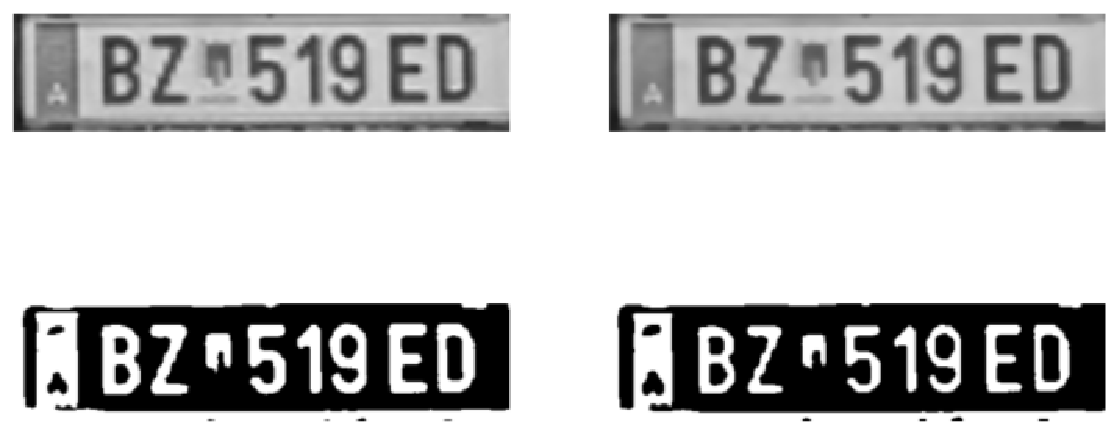
\includegraphics[width=0.9\linewidth]{kennzeichenerkennung/matplotlibvisual.pdf}
    \caption{Visualisierung mit Matplotlib}
\end{figure}

\paragraph{Modell für Zeichenerkennung laden und anwenden}\mbox{}\\

Für die Zeichenerkennung wird ein eigenes neuronales Netz verwendet, welches auf MobileNetV2 basiert. Dafür wird primär die Funktion „predict{\_}from{\_}model“ 
verwendet, welche im unteren Code ersichtlich ist.

\begin{listing}[H]
    \begin{minted}{python}
    def predict_from_model(image, model, labels):
        image = cv2.resize(image,(80, 80))
        image = npy.stack((image,)*3, axis = -1)
        prediction = labels.inverse_transform([npy.argmax (model.predict(image[npy.newaxis,:]))])
        return prediction
    \end{minted}
    \caption{predict{\_}from{\_}model}
\end{listing}

Vor der Anwendung dieser Funktion muss wieder, wie beim ersten Modell für maschinelles Lernen, das Modell zuerst geladen werden. Danach kann diese Funktion verwendet werden, 
welcher man das Bild eines Zeichens und das Model übergeben muss. Die Funktion „predict{\_}from{\_}model“ wendet dann nur dieses Modell an und übergibt das 
vermutete Ergebnis in ein Array.

\begin{longlisting}
    \begin{minted}{python}
    fig = mplt.figure(figsize = (15,3))
    cols = len(found_characters)
    grid = gridspec.GridSpec(ncols= cols, nrows= 1, figure = fig)

    result = ''
    for i, character in enumerate(found_characters):
        fig.add_subplot(grid[i])
        title = npy.array2string(predict_from_model(character, model, labels))
        mplt.title('{}'.format(title.strip("'[]"), fontsize=20))
        result += title.strip("'[]")
        mplt.axis(False)
        mplt.imshow(character, cmap='gray')

    print("-> License Plate:", result)
    \end{minted}
    \caption{Anwendung der Zeichenerkennung}
\end{longlisting}

Im oberen Bild sieht man die Anwendung der vorherigen Funktion. Prinzipiell wird für jedes vorher gefundene Zeichen das Modell angewendet 
und das Resultat von einem Array zu einem String konvertiert. Dieser String wird dann zum Ergebnis-String hinzugefügt, wodurch man am Ende das 
komplette Kennzeichen in einem String hat. Zusätzlich wird das komplette Kennzeichen mit den vermuteten Ergebnissen mit Matplotlib visualisiert. 
Dies ist im unteren Bild ersichtlich.

\begin{figure}[H]
    \centering
    
\includegraphics[width=0.9\linewidth]{kennzeichenerkennung/Ergebnisvisual.pdf}
    \caption{Visualisiertes Ergebnis der Kennzeichenerkennung}
\end{figure}

\paragraph{Resultat mittels API an Datenbank senden}\mbox{}\\

Wenn das Programm zu einem Resultat gekommen ist, muss dieses noch an die Datenbank übergeben werden. Der dafür zuständige Code ist im nächsten Codeteil ersichtlich.

\begin{longlisting}
    \begin{minted}{python}
    #API-Definitionen
    url = "http://dev.philipp-kraft.com/api/v1/detections"
    lp_result = {}
    lp_files = {}
    lp_result["name"] = result 
    lp_result["parking_lot_id"] = "2"   #Parkplatz-ID 
    lp_files=[
    ('image',('kennzeichen.png',open('lp_image/lp.png','rb'),'image/png'))
    ]
    header = {"Authorization": "Bearer 5|4NcJgCrR9FkeTFeTvRGHLQqoJBeY8IDqxborpuuS"}

    #Senden der Daten an die Datenbank und Ausgabe der Response
    resp = requests.post(url, data=lp_result, files=lp_files, headers=header)
    print("-> API-Response:",resp.text)
    \end{minted}
    \caption{Senden der Ergebnisse an die Datenbank}
\end{longlisting}

Im ersten Schritt werden die URL für die API und für die Ergebnisse zwei Dictionaries erstellt. In das erste Dictionary wird der String für das Kennzeichen 
und die ID-Nummer des Parkplatzes eingetragen. In das zweite Dictionary kommt das Bild des Kennzeichens. Im nächsten Schritt muss noch ein Bearer Token 
definiert werden, welcher auf der APM-Website generiert werden kann. Dieser wird zur Autorisierung benötigt. Danach können diese Daten über einen Post-Befehl 
an die API gesendet werden. Um den Status dieser Kommunikation zu überprüfen wird im Anschluss noch die Antwort der API im Terminal ausgegeben. Bei 
erfolgreicher Kommunikation antwortet diese mit dem aktuellen Status des Fahrzeuges auf dem Parkplatz.

\subsection{Raspberry Pi}

\subsubsection{Einleitung}
Damit die Software der Kennzeichenerkennung arbeiten kann, benötigt es eine geeignete Hardware. Diese muss dabei die folgenden Eigenschaften 
aufweisen, um für die Kennzeichenerkennung geeignet zu sein:

\begin{itemize}
    \item Möglichst klein
    \item Nicht zu teuer 
    \item Möglichkeit eine Kamera anzuschließen 
    \item Schnell 
    \item Internetanbindung
\end{itemize}

\subsubsection{Wahl des Raspberry Pi}
In dieser Applikation wird ein Raspberry Pi 4B 2GB verwendet, da er alle zuvor genannten Eigenschaften am besten erfüllt.\\

\begin{figure}[H]
    \centering
    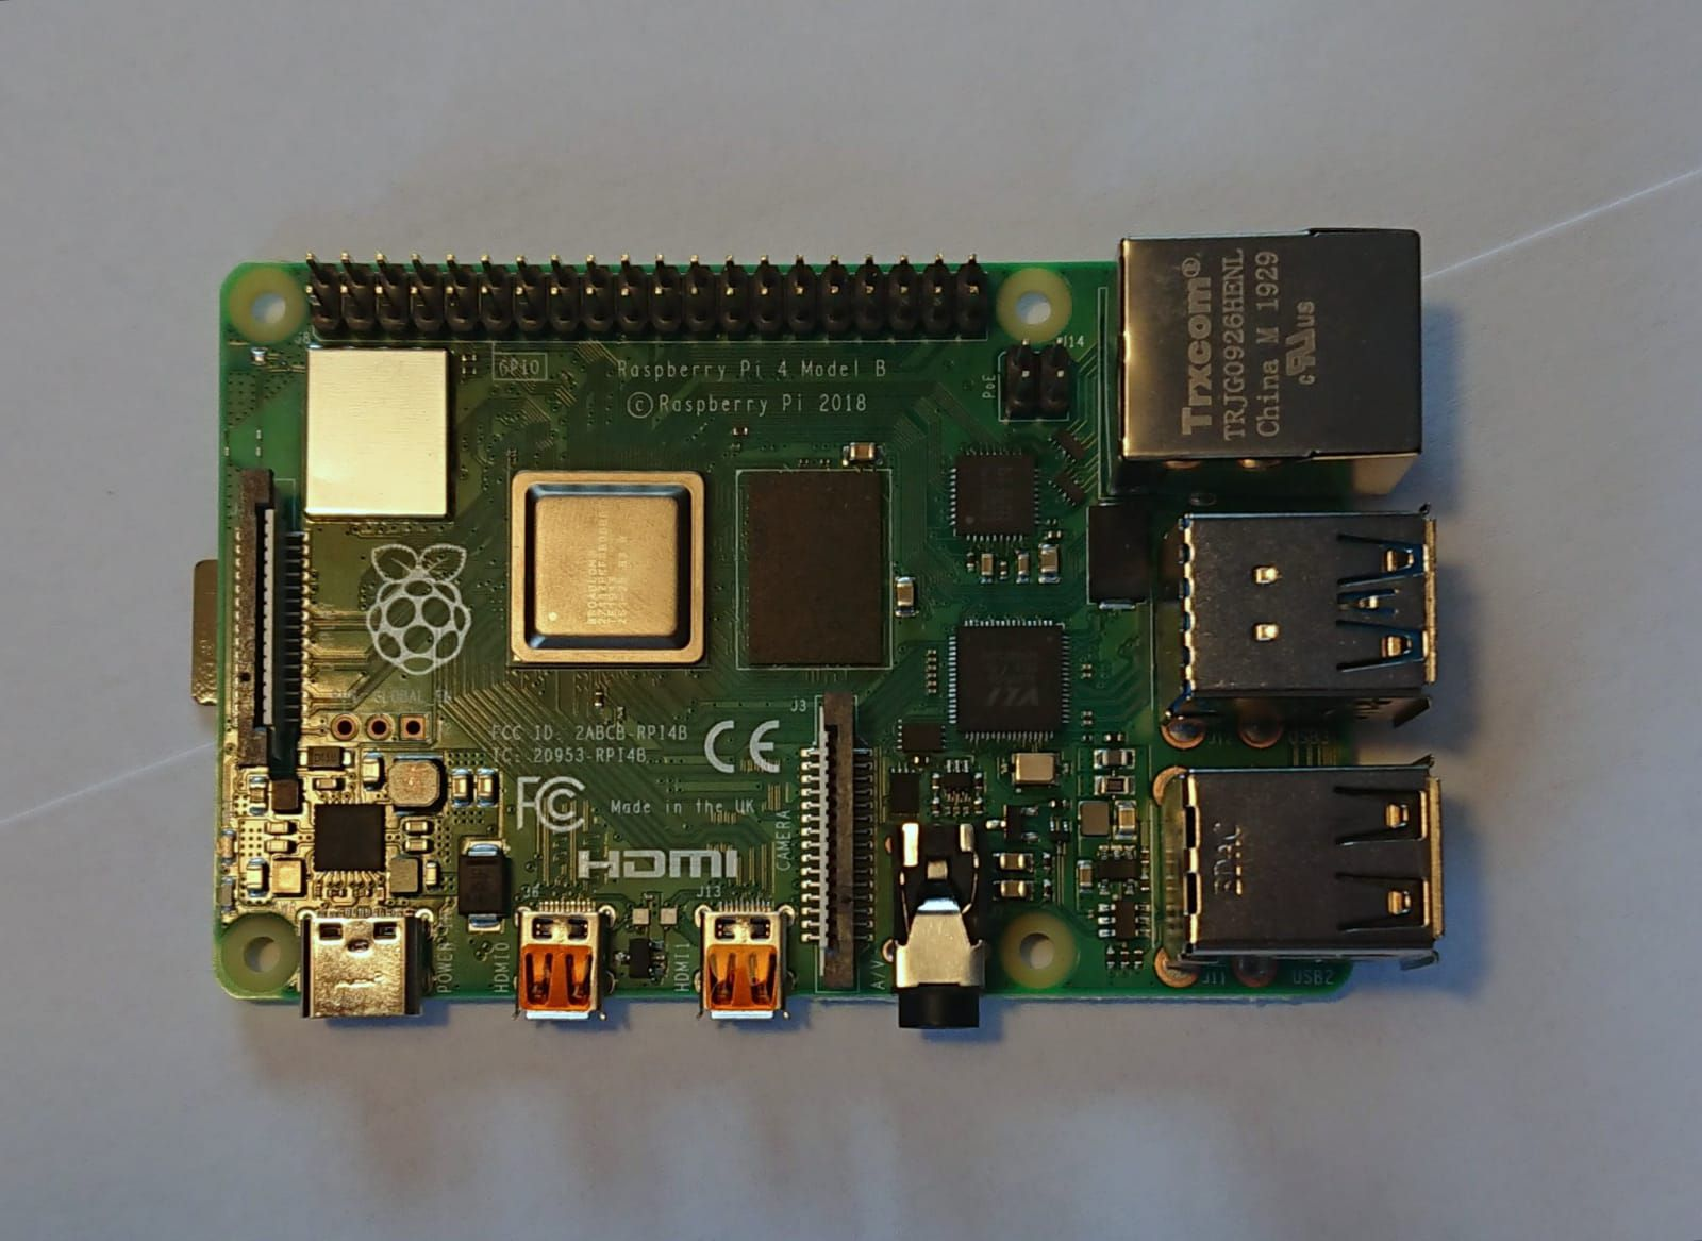
\includegraphics[width=0.6\linewidth]{kennzeichenerkennung/rpi.pdf}
    \caption{Raspberry Pi}
\end{figure}

Er hat die Größe einer Scheckkarte, wodurch es möglich ist ein kompaktes Gehäuse zu bauen, welches man einfach montieren kann. 
Er ist mit 35€ pro Stück nicht zu teuer. Er hat einen integrierten Kameraanschluss und es gibt unzählige Kameras, welche damit 
kompatibel sind. Er hat für seine Größe eine sehr gute Rechenkraft und ist damit in der Lage das komplette Programm für die 
Kennzeichenerkennung in einer akzeptablen Zeit abzuarbeiten. Er besitzt außerdem einen Ethernet-Anschluss und ein WLAN-Modul, 
wodurch er sehr einfach mit dem Internet verbunden werden kann.

\subsubsection{Kamera}
Für den Raspberry Pi muss zudem noch die passende Kamera ausgewählt werden, um die Bilder von den Kennzeichen aufzunehmen. 
Dafür gibt es Unmengen an kompatiblen Kameras, aber hier wird das Originalzubehör von Raspberry Pi verwendet. Dies hat den Grund, 
dass diese Kamera leicht zu verwenden, sehr klein, mit Schrauben einfach zu befestigen und günstig ist. Zudem liefert sie ein 
qualitativ hochwertiges Bild, welches für die Software gut verarbeitbar ist.

\begin{figure}[H]
    \centering
    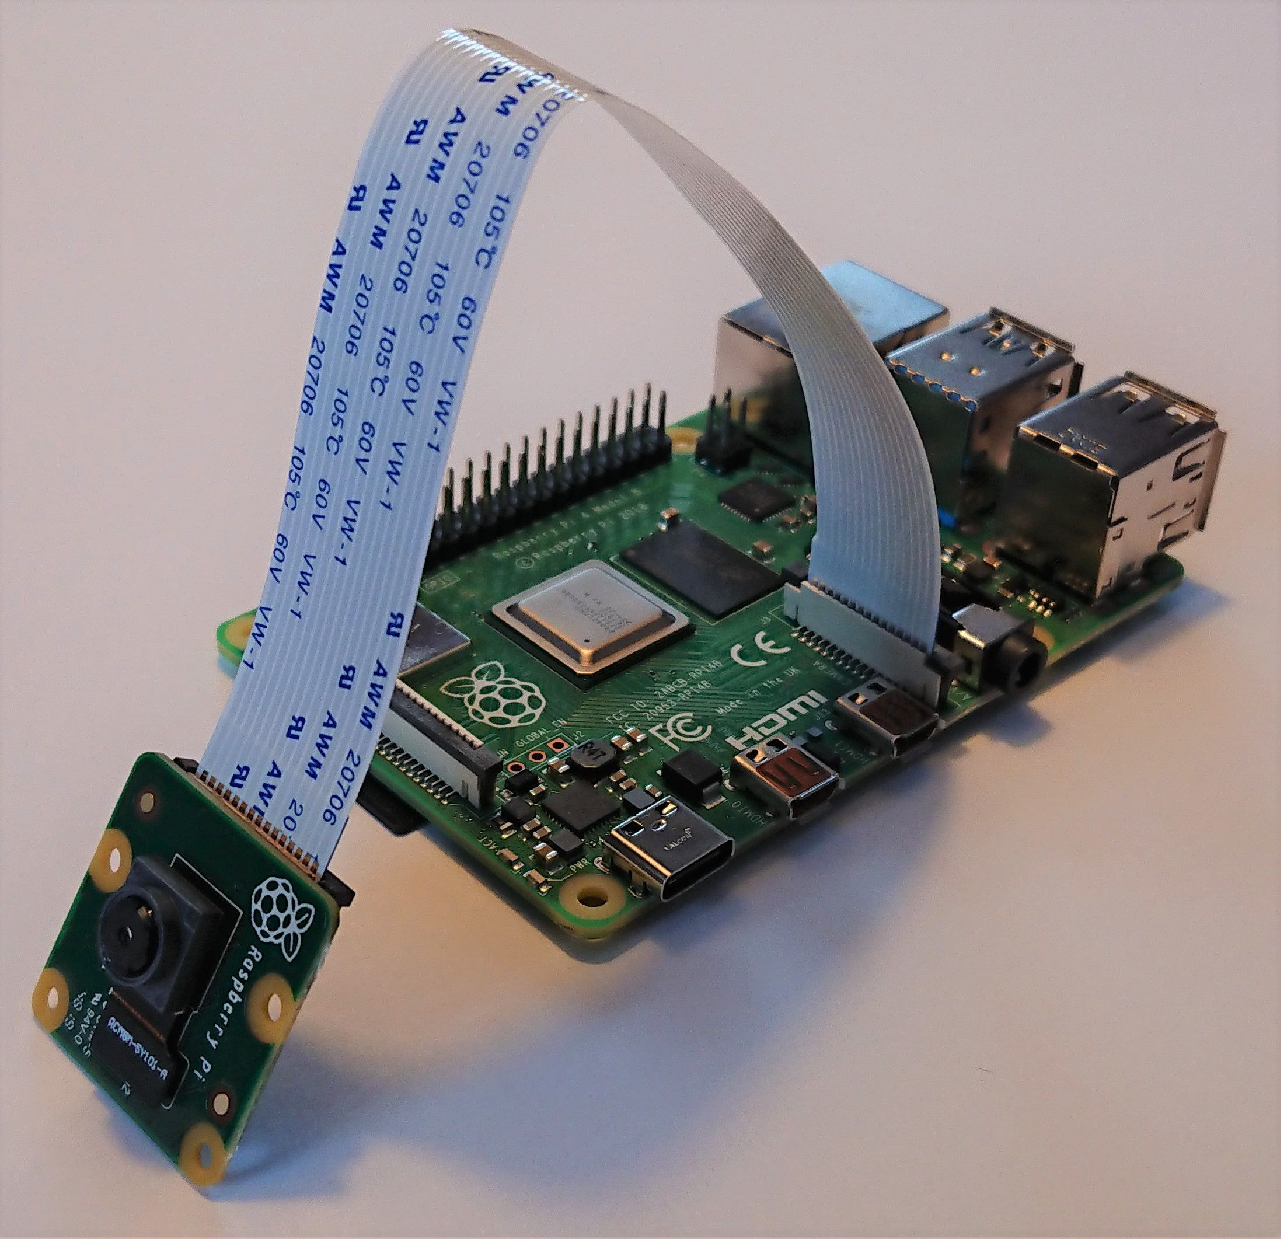
\includegraphics[width=0.6\linewidth]{kennzeichenerkennung/rpiKamera.pdf}
    \caption{Raspberry Pi mit Kamera}
\end{figure}

\subsection{Maschinelles Lernen}

\subsubsection{Einleitung}
Die Kennzeichenerkennung ist eine sehr komplexe Anwendung, da es unzählige Kennzeichen gibt und jedes einzelne davon erkannt werden sollte. 
Dabei ist nicht nur auf verschiedene Länderkennzeichen zu achten, welche sich stark voneinander unterscheiden, sondern auch auf Sonderkennzeichen, 
welche sich sogar auf nationaler Ebene von den normalen Kennzeichen unterscheiden. Zudem besteht noch die Problematik, dass sich die Kennzeichen 
oft in unterschiedlichen Zuständen befinden, wie zum Beispiel mit Staub beschmutzt oder ähnliches. Das bedeutet, dass eine in der Praxis 
anwendbare Kennzeichenerkennung mit all diesen Gegebenheiten zurechtkommen muss, damit das Kennzeichen in nahezu jeder möglichen Situation 
erkannt wird. Um dies zu erreichen wird das Programm für die Kennzeichenerkennung in drei größere Teile aufgeteilt. Die Kennzeichenlokalisierung, 
die Zeichenerfassung und die Zeichenerkennung. Die Zeichenerfassung gestaltet sich relativ einfach, da diese bereits ein Bild des Kennzeichens erhält, 
in dem ansonsten keine größeren Störfaktoren beinhaltet sind. Diese muss also nur die Konturen innerhalb dieses Bildes finden und diese so sortieren, 
dass nur noch die einzelnen Zeichen übrig bleiben. Bei der Kennzeichenlokalisierung und der Zeichenerfassung gestaltet sich die Lage schon etwas schwieriger. 
Die Kennzeichenlokalisierung steht vor dem Problem, dass wenn man klassisch mit der Bildverarbeitung nach einer passenden Kontur für das Kennzeichen sucht, 
kann dieser Algorithmus durch Störfaktoren wie ein zufällig ähnlich großes Orts- oder Straßenschild getäuscht werden, wodurch es zu einem Fehler kommt. 
Auch Fenster oder ähnlich proportionierte Gegenstände können zu solch einem Fehler führen. Die Lösung dafür befindet sich im Bereich des maschinellen Lernens. 
Anstatt nur nach einer Kontur zu suchen, wird mit solch einem Modell gezielt nach einem Kennzeichen gesucht. Dies ist möglich, da so ein Modell mit vielen 
möglichen Eingaben und den passenden Ausgaben dazu trainiert wird ein Muster zwischen den Ein- und Ausgaben zu finden, mit welchem es dann ähnliche Probleme 
selbstständig lösen kann. Auch bei der Zeichenerkennung bietet sich solch ein Modell an, da es darauf trainiert werden kann, einzelne Zeichen mit einer 
hohen Genauigkeit zu erkennen. Hier wäre es zwar ohne maschinelles Lernen auch möglich ein relativ gutes Ergebnis zu erzielen, indem man mittels Korrelation 
von Vergleichsbildern das Zeichen findet, welches am wahrscheinlichsten passen würde, aber in dieser Applikation wird auch hierfür ein Modell für maschinelles Lernen verwendet.

\subsubsection{Definition}
Maschinelles Lernen beschreibt ein Modell, welches zuerst in einer Trainingsphase trainiert werden muss, um danach ähnliche Probleme näherungsweise lösen zu können. 
Dazu wird in der Trainingsphase ein Datensatz bereitgestellt welcher mögliche Eingaben und meistens auch die passenden Ausgaben enthält. Durch die vielen verschiedenen 
Eingaben und Ausgaben ist es für das Modell möglich ein Muster zwischen diesen zu erkennen, welches durch dieses Training verbessert werden kann. Es gilt dabei, je 
länger die Trainingsphase dauert, desto genauer wird das Modell. Der Aufwand besteht dabei darin, die gigantischen Datensätze zur Verfügung zu stellen, da diese oft 
zuvor erstellt werden müssen. Zudem ist das Training ein sehr rechenintensiver Vorgang, welcher für ein gutes Ergebnis oft mehrere Stunden benötigt. In den letzten 
Jahren hat sich im Bereich des Modell Trainings eine neue Entwicklung namens „Deep Learning“ verbreitet, mit welcher eine höhere Genauigkeit als mit bisherigen Modellen 
erreicht werden kann. Dabei werden künstliche neuronale Netze erstellt, welche der Vernetzung von Neuronen in Lebewesen nachempfunden sind. Diese künstlichen Neuronen 
sind Verknüpfungspunkte zwischen Eingang und Ausgang des Modells und sind je nach Komplexität in verschiedene Schichten aufgeteilt. Um diese künstlichen Neuronen zu 
trainieren, werden deren Gewichtungswerte angepasst. Deswegen muss bei solchen Modellen auch oft eine Datei mit den gewichteten Werten eingebunden werden. In der unteren Abbildung ist
eine vereinfachte Darstellung eines mehrschichtigen neuronalen Netzes erkennbar.

\begin{figure}[H]
    \centering
    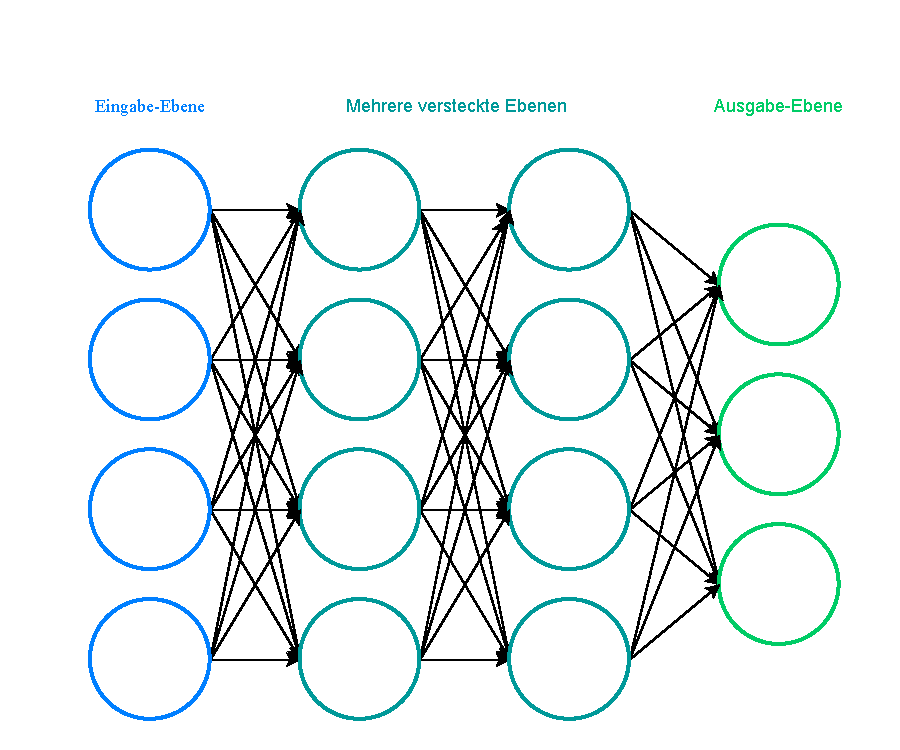
\includegraphics[width=0.9\linewidth]{kennzeichenerkennung/neural.pdf}
    \caption{Mehrschichtiges neuronales Netz}
\end{figure}

\subsubsection{Vergleich maschinelles Lernen / Bildverarbeitung}
Zum Beginn dieser Applikation wurde ein Ansatz ohne den Einsatz von maschinellem Lernen verfolgt. Dazu wurde ein Testprogramm geschrieben, welches das Kennzeichen 
über eine Konturerkennung lokalisieren sollte. Dies führte aber zu häufig auftretenden Fehlern. Einer dieser Fehler ist in der unteren Abbildung ersichtlich.

\begin{figure}[H]
    \centering
    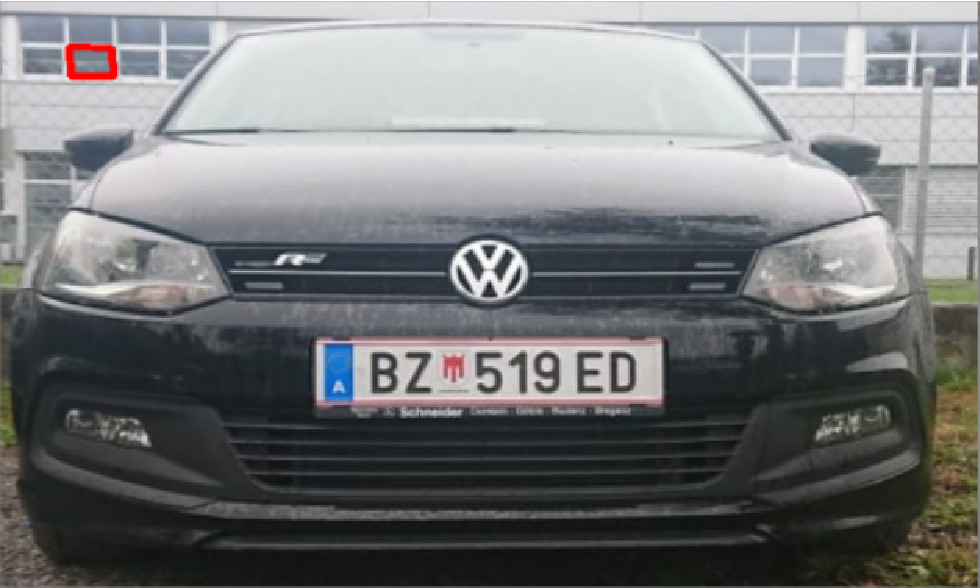
\includegraphics[width=0.9\linewidth]{kennzeichenerkennung/bildvtestfehler.pdf}
    \caption{Fehler bei Konturerkennung}
\end{figure}

Wie in der oberen Abbildung erkennbar ist, hat das Programm nicht das Kennzeichen erkannt, sondern ein Fenster im Hintergrund, welches eine ähnliche Kontur 
wie das Kennzeichen aufweist. Dies ist deswegen aufgetreten, da das Kennzeichen über seine Kontur gefunden werden sollte und dazu alle Konturen im Bild aufgelistet 
werden und aus dieser Liste dann das Kennzeichen herausgesucht werden sollte. Dies führte in dieser Testversion aber nahezu nie zu einem Ergebnis, welches in 
der Praxis anwendbar gewesen wäre. Durch eine Anpassung der Software wäre es zwar möglich gewesen die Genauigkeit zu verbessern und dafür zu sorgen, dass mit 
einer größeren Wahrscheinlichkeit die richtige Kontur ausgewählt wird, aber bei einer Kontur mit den gleichen Proportionen wie ein Kennzeichen, wäre die Konturerkennung 
wieder schnell an ihre Grenzen gestoßen. Deswegen wurde der Ansatz komplett verändert und für die Kennzeichenlokalisierung ein Modell für maschinelles Lernen 
verwendet, welches auf deutlich elegantere und effizientere Weise ein besseres Resultat erzielen kann.

\begin{figure}[H]
    \centering
    
\includegraphics[width=0.5\linewidth]{kennzeichenerkennung/kennmaschinlearn.pdf}
    \caption{Resultat mit maschinellem Lernen}
\end{figure}

Zum Vergleich mit dem Testprogramm sieht man im oberen Bild das Ergebnis der Variante mit maschinellem Lernen mit demselben Eingangsbild. Dabei wurde ohne 
Probleme das Kennzeichen perfekt erkannt und im weiteren Programmablauf aus dem Eingangsbild ausgeschnitten.

\subsubsection{Verwendete Modelle für maschinelles Lernen}

\paragraph{WPOD-NET}\mbox{}\\
Das „Warped Planar Object Detection Network“ (WPOD-NET) ist ein künstliches neuronales Netz, welches von Sérgio Montazolli Silva und 
Cláudio Rosita Jung\footnote{\cite{wpodnet}}
entwickelt wurde. Es wurde entwickelt, um aus Bildern die Kennzeichen von Fahrzeugen herauszusuchen und bietet im Gegensatz zu anderen Modellen den entscheidenden 
Vorteil, dass es bei diesem Modell irrelevant ist aus welchem Winkel das Bild vom Kennzeichen aufgenommen wird. Andere Modelle funktionieren oft nur wenn das Foto 
vom Kennzeichen direkt von vorne aufgenommen wurde, da ansonsten das Bild verzerrt wird und dadurch das Kennzeichen nicht mehr ausgelesen werden kann. Dieses Modell 
schafft es auch aus einem von der Seite aufgenommen Bild, das Kennzeichen in den meisten Fällen gut genug herauszulesen, dass dieses Bild danach weiterverarbeitet 
werden kann. Dies bietet den Vorteil, dass die Kamera für das Gerät nicht fix verbaut werden muss, sondern theoretisch auch in einem mobilen Gerät installiert werden kann.\\

Die Kennzeichenerkennung dieses Modells basiert auf zwei Schritten. Zuerst wird im Bild nach einem Fahrzeug gesucht und dieses ausgeschnitten, um danach mit 
WPOD-NET das Kennzeichen aus diesem Bild herauszusuchen. Die Fahrzeugerkennung basiert dabei auf dem 
YOLOv2 Netzwerk, 
welches für Echtzeitobjekterkennung verwendet wird und neben vielen anderen Gegenständen auch in der Lage ist Fahrzeuge in beliebiger Lage zu erkennen. Nach dieser Fahrzeugerkennung wird das Bild in das WPOD-NET eingegeben.

\begin{figure}[H]
    \centering
    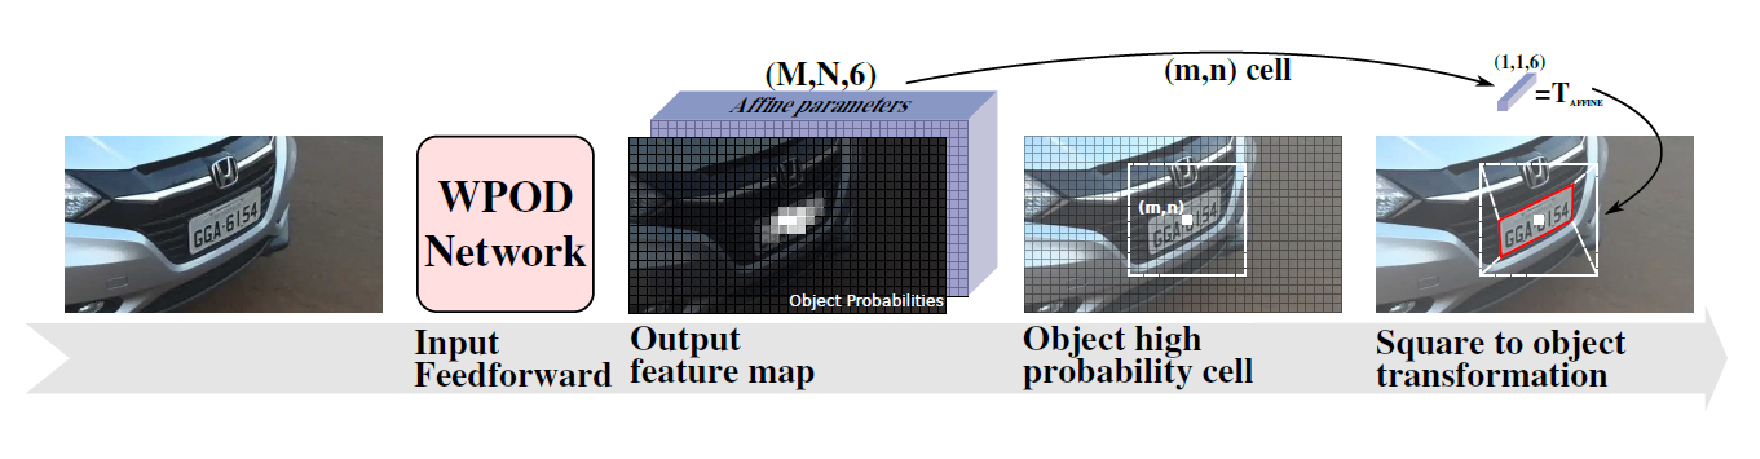
\includegraphics[width=0.9\linewidth]{kennzeichenerkennung/wpodnet.pdf}
    \caption{Ablauf von WPOD-NET, \cite{wpodnet}}
\end{figure}

Im oberen Bild ist der prinzipielle Ablauf der Kennzeichenerkennung ersichtlich. Zu Beginn wird das Bild mit dem Kennzeichen in das WPOD-NET eingegeben 
und dieses gibt dann eine Matrix mit gewichteten Werten zurück, welche für jede einzelne Zelle eine Wahrscheinlichkeit angibt, dass sich dort ein Kennzeichen 
befindet. Um die Zelle, die am wahrscheinlichsten ist, wird dann ein Rechteck gespannt in welchem sich mit sehr hoher Wahrscheinlichkeit das Kennzeichen 
befindet. Danach wird auf die Wahrscheinlichkeitswerte für das gesamte Rechteck Thresholding angewandt, um zu bestimmen in welchen Zellen sich das Kennzeichen 
befindet. Dadurch hat man dann diejenige Region gefunden, in der sich das Kennzeichen befindet und kann dieses, wenn nötig in ein horizontal und vertikal 
ausgerichtet Rechteck umwandeln. Dadurch erhält man dann ein Bild des Kennzeichens.

\paragraph{MobileNetV2}\mbox{}\\
MobileNetV2\footnote{\cite{MobileNet}} ist die Grundlage für das eigene trainierte neuronale Netz. MobileNetV2 ist eine Grundlage für diverse neuronale Netze und speziell für Anwendungen im Bereich der Computer Vision 
geeignet. Einige Beispiel dafür sind die Erkennung von Gesichtsmerkmalen, Echtzeitobjekterkennung, Unterscheidung diverser Hunderassen oder ähnliches. Dabei ist das Modell je nach Bedürfnissen 
einstellbar, womit für eine schnellere und bessere Leistung weniger Schichten für das neuronale Netz verwendet werden, oder aber für eine sehr genaue und präzise Funktion mehr Schichten verwendet werden. 
Dies ist dadurch möglich, dass das Netzwerk auf einer variablen Schichtanzahl aufgebaut ist. In dieser Applikation wird es deswegen verwendet, da damit in diesem Bereich eine hohe Präzision erzielbar ist, 
welche für die Kennzeichenerkennung benötigt wird.

\subsection{Modell Training}
Um das Modell für die Zeichenerkennung zu trainieren wurde ein eigenes Programm geschrieben, welches das Modell mittels Tensorflow trainiert. 
Dazu wird ein Datensatz von 35 000 Bildern von Zeichen verwendet, bei welchen die richtige Ausgabe aus dem Dateiname auslesbar ist. 
Im folgenden Bild sieht man ein Beispiel für so ein Bild aus dem Datensatz.

\begin{figure}[H]
    \centering
    
\includegraphics[width=0.2\linewidth]{kennzeichenerkennung/S.pdf}
    \caption{Beispiel eines Zeichens aus dem Datensatz}
\end{figure}

Das Modell wird durch die verschiedenen Schriftarten und die variierende Qualität der Bilder nicht direkt auf die Erkennung von Zeichen aus 
einem Kennzeichen trainiert, sondern auf die Erkennung von Zeichen in jeglicher Situation. Dies benötigt zwar länger, um das Modell zu trainieren, 
aber es ist dadurch genauer und kann auch in anderen Anwendungen ohne größere Umstellungen verwendet werden.\\

In den nächsten Codeteilen sieht man ein paar wichtige Ausschnitte aus dem Code für das Modell Training.

\begin{longlisting}
    \begin{minted}{python}
    def create_model(lr=1e-4,decay=1e-4/30, training=False,output_shape=y.shape[1]):
        baseModel = MobileNetV2(weights="imagenet", include_top=False, input_tensor=Input(shape=(80, 80, 3)))

        headModel = baseModel.output
        headModel = AveragePooling2D(pool_size=(3, 3))(headModel)
        headModel = Flatten(name="flatten")(headModel)
        headModel = Dense(128, activation="relu")(headModel)
        headModel = Dropout(0.5)(headModel)
        headModel = Dense(output_shape, activation="softmax")(headModel)

        model = Model(inputs=baseModel.input, outputs=headModel)

        if training:
            for layer in baseModel.layers:
                layer.trainable = True
            optimizer = Adam(lr=lr, decay = decay)
            model.compile(loss="categorical_crossentropy", optimizer=optimizer, metrics=["accuracy"])
    
        return model
    \end{minted}
    \caption{Erstellen des Modells basierend auf MobileNetV2}
\end{longlisting}

Im ersten Teil sieht man das grundlegende Erstellen des Modells auf der Grundlage von MobileNetV2. Zusätzlich werden noch die Einstellungen für 
Tensorflow getroffen wie zum Beispiel die Größe der Eingabe und weitere Parameter, welche von Tensorflow für die Erstellung des Modells benötigt wird. 
Im unteren Teil wird noch definiert welcher Optimierer verwendet werden soll und dass während des Trainings die Genauigkeit des Modells aufgenommen werden soll.

\begin{longlisting}
    \begin{minted}{python}
    INIT_LR = 1e-4
    EPOCHS = 30

    model = create_model(lr=INIT_LR, decay=INIT_LR/EPOCHS, training=True)

    BATCH_SIZE = 64

    my_checkpointer = [EarlyStopping(monitor='val_loss', patience=5, verbose=0), ModelCheckpoint(filepath="License_character_recognition.h5", verbose=1, save_weights_only=True)]
    result = model.fit(image_gen.flow(trainX, trainY, batch_size=BATCH_SIZE), 
                        steps_per_epoch=len(trainX) // BATCH_SIZE, 
                        validation_data=(testX, testY), 
                        validation_steps=len(testX) // BATCH_SIZE, 
                        epochs=EPOCHS, callbacks=my_checkpointer)
    \end{minted}
    \caption{Trainieren des Modells und Einstellungen anpassen}
\end{longlisting}

Im zweiten Teil wird zuerst die Standard Lernrate des Modells und die Anzahl der Epochen definiert. Die Epochen sind eine Art Meilenstein, 
nach welchem die Genauigkeit dargestellt und beurteilt wird, um den Trainingserfolg zu beurteilen. Außerdem werden nach jeder Epoche die gewichteten Werte 
angepasst und abgespeichert. Danach wird noch eingestellt nach welcher Anzahl an Epochen ohne signifikante Verbesserung das Training frühzeitig 
beendet werden soll, und wohin die gewichteten Werte abgespeichert werden sollen. Danach werden Tensorflow die Daten übergeben, um das Training 
zu beginnen. Die Dauer dieses Vorgangs unterscheidet sich von Computer zu Computer, und hat bei dieser Applikation in etwa 10 Stunden gedauert.\\

Im nächsten Bild sieht man den Trainingsverlauf des Modells über 30 Epochen.

\begin{figure}[H]
    \centering
    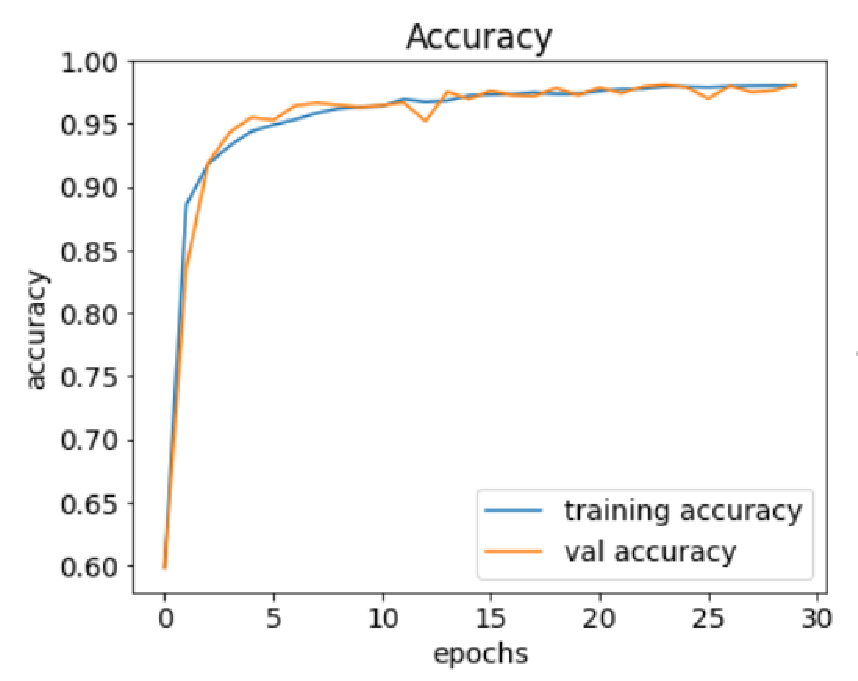
\includegraphics[width=0.7\linewidth]{kennzeichenerkennung/trainingsverlauf.pdf}
    \caption{Verlauf des Modell Trainings}
\end{figure}

Im oberen Bild kann man erkennen, dass die Genauigkeit des Modells bereits nach wenigen Epochen einen Wert von über 90\% erreicht hat und 
nach den 30 Epochen auf einen Endwert von 98,02\% erreicht hat. Das bedeutet, dass bei einem Kennzeichen mit durchschnittlich 7 Zeichen 
eine insgesamte Genauigkeit von 86,93\% erreicht wird. Diese Genauigkeit könnte mit einem längeren Training theoretisch auf einen Wert von 
nahezu 100\% gesteigert werden, aber dazu benötigt es einen stärkeren Computer, welcher zudem noch eine ganze Weile nicht benutzt werden kann.

\subsection{Gehäuse}

\subsubsection{Anforderungen}
Die Anforderungen an das Gehäuse sind recht simpel. Es soll das Modul vor äußeren Einwirkungen schützen, eine Möglichkeit bieten, 
um die Kamera des Raspberry Pi zu befestigen und für weitere Test- und Entwicklungszwecke soll der Zugang zu den wichtigsten Anschlüssen des Raspberry Pi ermöglicht werden, damit diese verwendet werden können. Zudem sollen die Entwicklungs- und Produktionskosten eher gering sein, weswegen sich ein 
Gehäuse aus dem 3D-Drucker am besten eignet.

\subsubsection{Umsetzung}
Das 3D-Modelling des Gehäuses erfolgte mit dem Programm „Autodesk Fusion 360“\footnote{\url{https://www.autodesk.de/products/fusion-360/overview}}, mit welchem 3D-Modelle erstellt und konvertiert werden können, 
damit man sie mit dem 3D-Drucker ausdrucken kann. In den folgenden Bildern sieht man die Renderansichten der einzelnen Teile.

\begin{figure}[H]
    \centering
    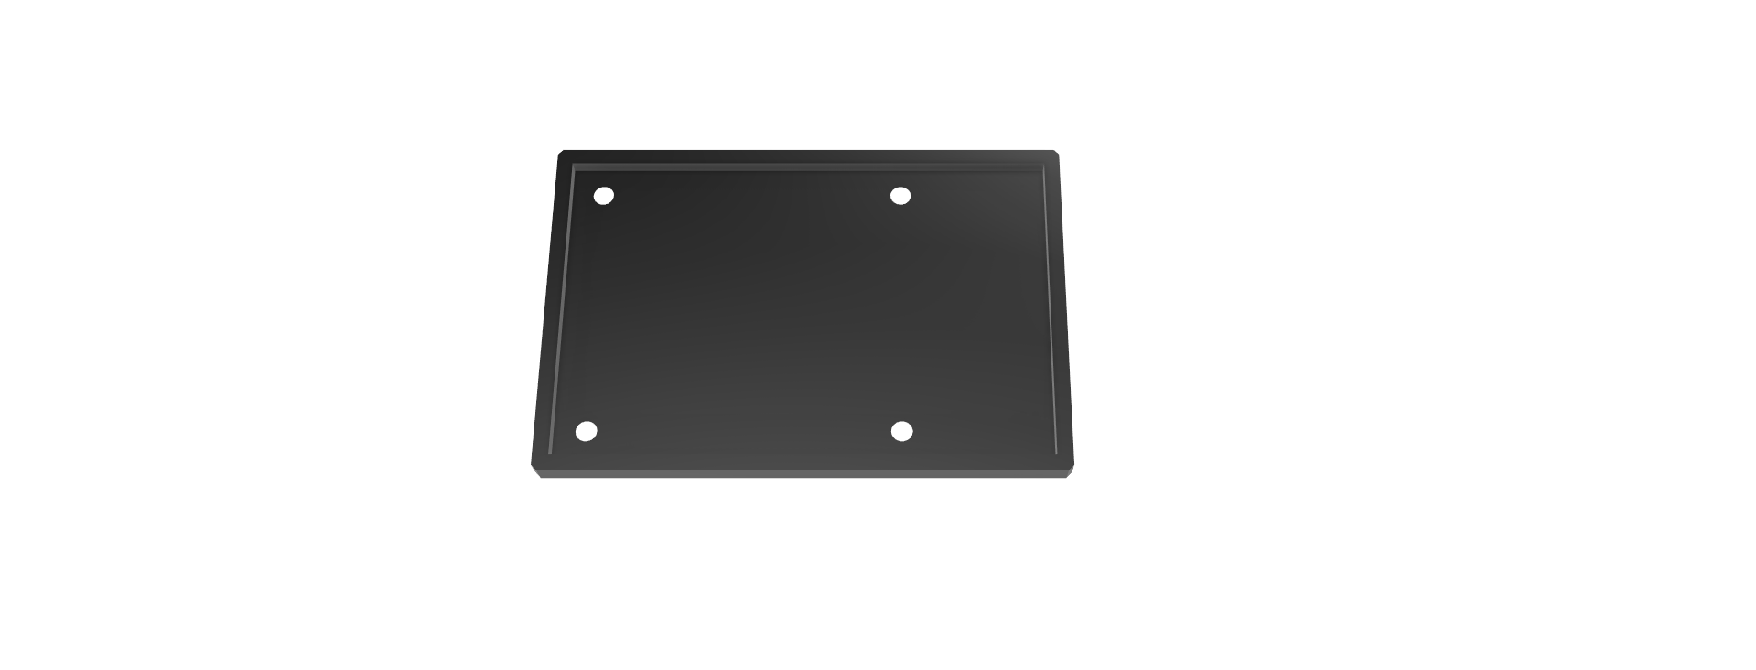
\includegraphics[width=1\linewidth]{kennzeichenerkennung/Renderboden.pdf}
    \caption{Boden des Gehäuses}
\end{figure}

Im ersten Bild sieht man die Renderansicht des Bodens. Auf diesen wird der Raspberry Pi gelegt und mit den 4 Bohrungen an den mittleren Teil geschraubt. 
Dadurch ist der Raspberry Pi sicher befestigt und kann im Gehäuse nicht verrutschen.

\begin{figure}[H]
    \centering
    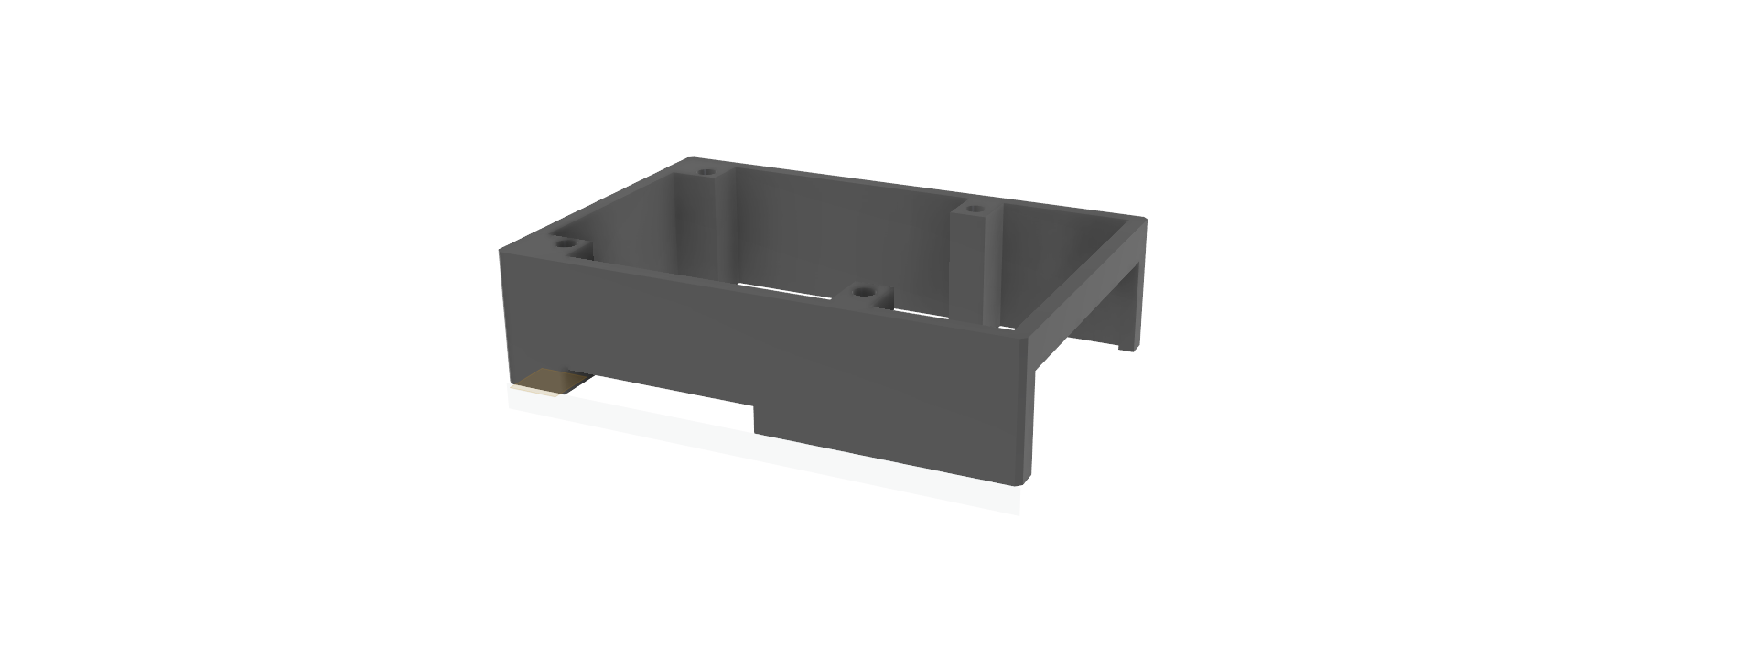
\includegraphics[width=1\linewidth]{kennzeichenerkennung/Rendermittel.pdf}
    \caption{Mittelteil des Gehäuses}
\end{figure}

Der mittlere Teil besitzt 4 Verstärkungen auf der inneren Seite, in welche man Gewinde einfügen kann. Dadurch können der Deckel und der Boden angeschraubt werden. 
Zudem befinden sich auf zwei Seiten Ausschnitte durch welche die Stromversorgung, die HDMI-Ports, die USB-Ports und der Ethernet-Anschluss des Raspberry Pi 
zugänglich sind. Dadurch kann der Raspberry Pi nahezu ohne Einschränkungen mit den wichtigsten Funktionen betrieben werden.

\begin{figure}[H]
    \centering
    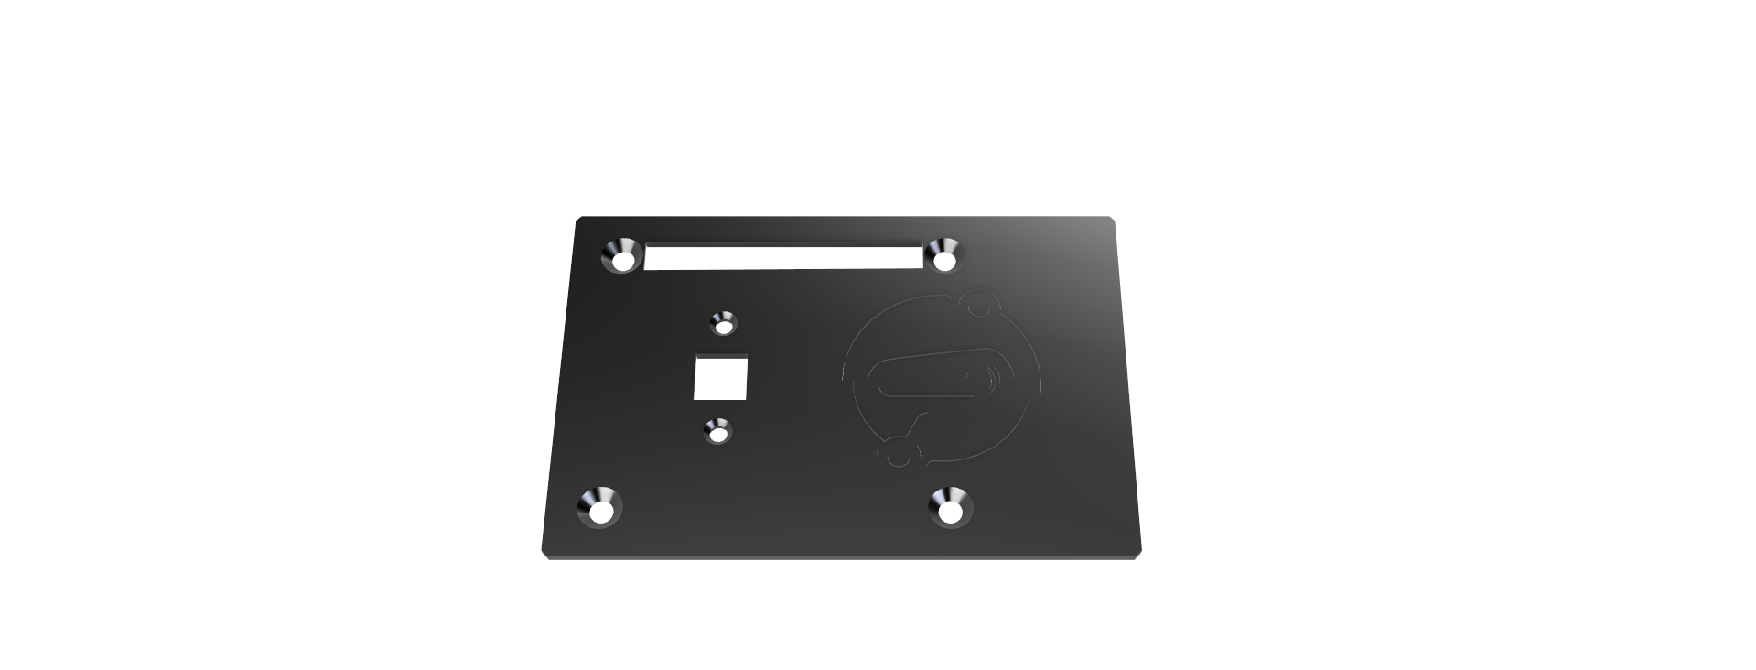
\includegraphics[width=1\linewidth]{kennzeichenerkennung/Renderdeckel.pdf}
    \caption{Deckel des Gehäuses}
\end{figure}

Das letzte Einzelteil ist der Deckel, welcher wieder die gleichen 4 Bohrungen wie der Boden aufweist, um mit dem Mittelteil verschraubt zu werden. 
Zusätzlich befinden sich im Deckel noch zwei Bohrungen, um die Kamera festzuschrauben und eine rechteckiges Aussparung, durch welches die Kamera gesteckt werden kann. 
Außerdem befindet sich auf dem Deckel noch das eingravierte Logo von APM. In der nächsten Abbildung sieht man dann noch eine Gesamtansicht des Gehäuses.

\begin{figure}[H]
    \centering
    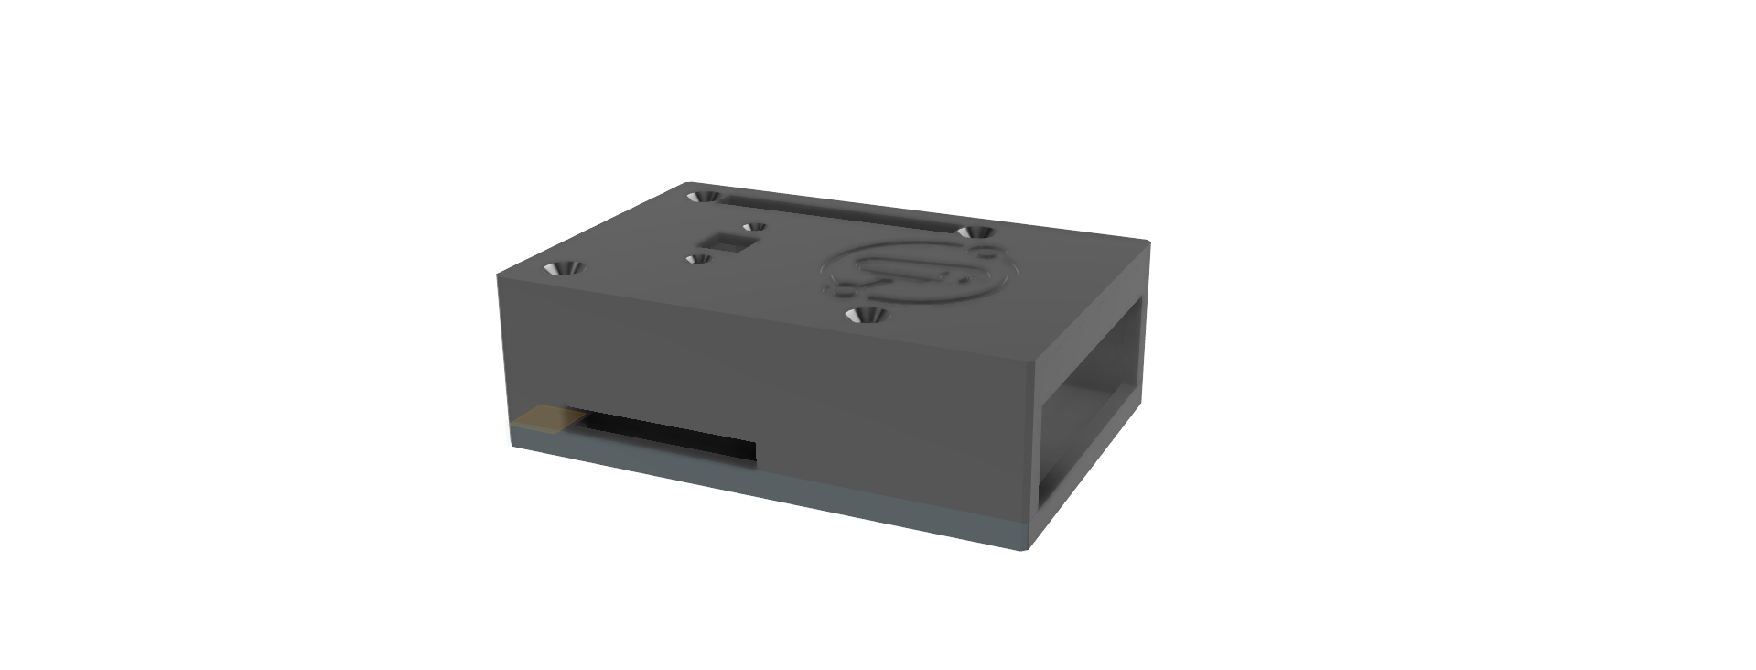
\includegraphics[width=1\linewidth]{kennzeichenerkennung/Rendergesamt.pdf}
    \caption{Gesamtesansicht des Gehäuses}
\end{figure}

Diese Einzelteile wurden dann mit einem 3D-Drucker gefertigt. In den nächsten Bildern sieht man die einzelnen gefertigten Teile und eine Gesamtansicht.

\begin{figure}[H]
    \centering
    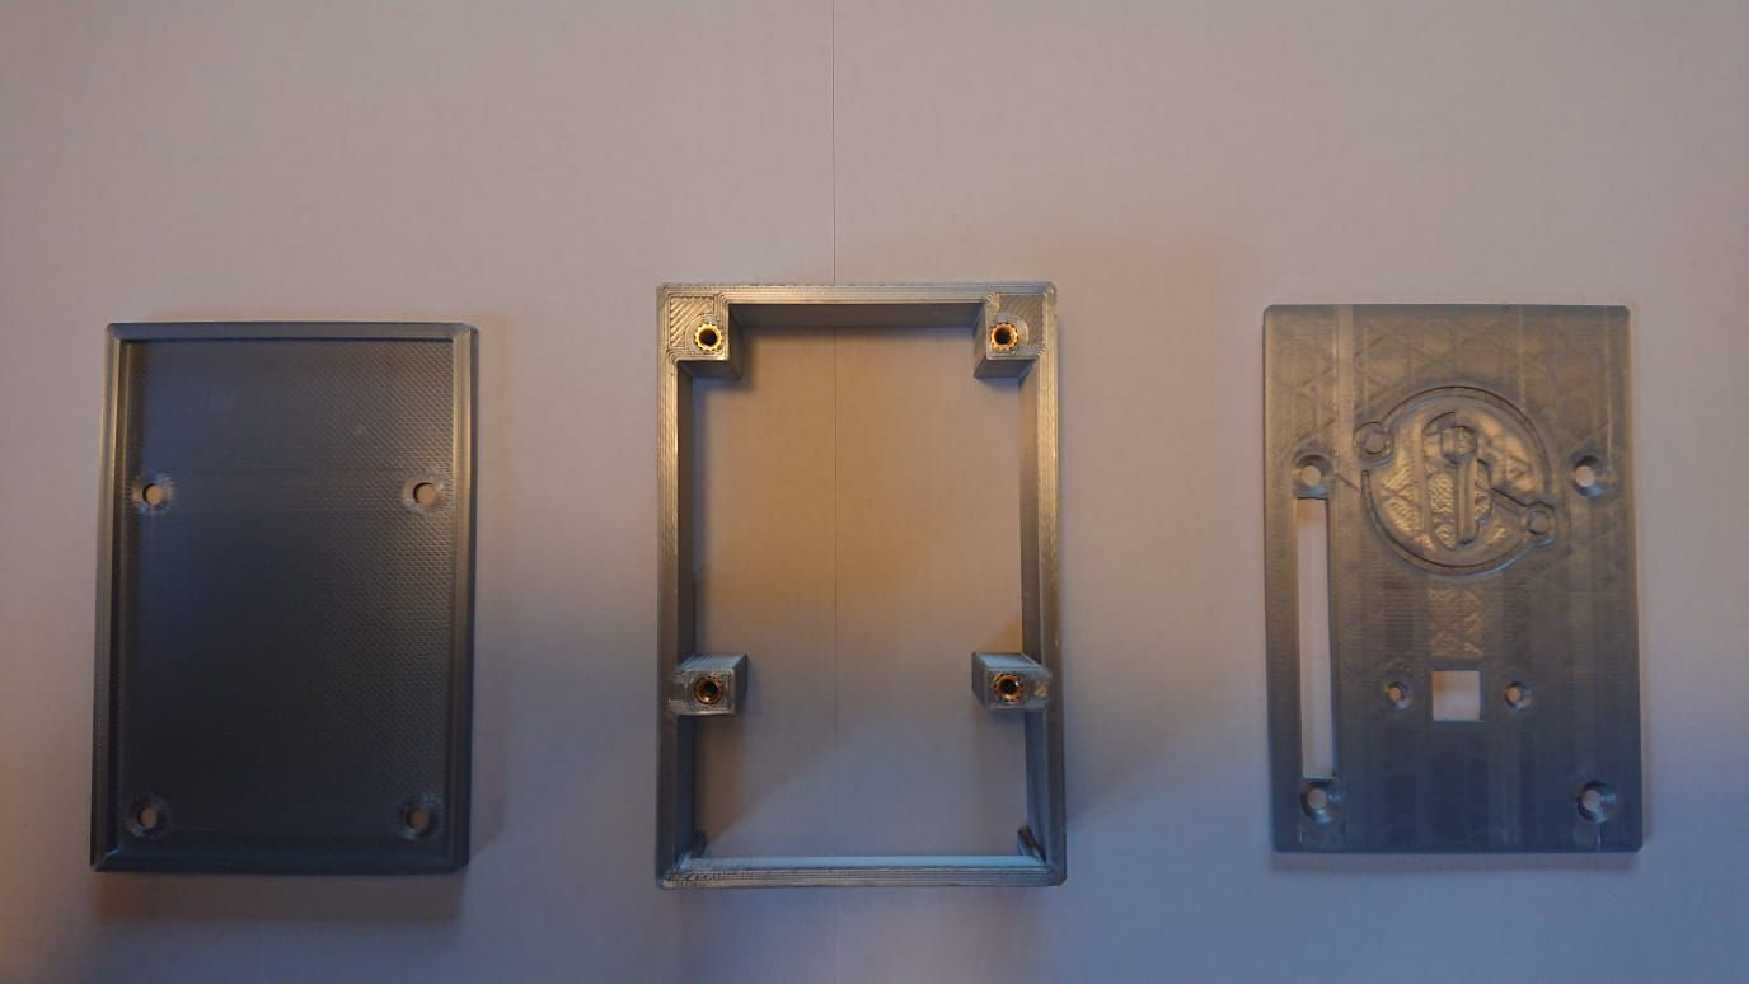
\includegraphics[width=0.8\linewidth]{kennzeichenerkennung/geinzel.pdf}
    \caption{Gedruckte Einzelteile des Gehäuses}
\end{figure}

\begin{figure}[H]
    \centering
    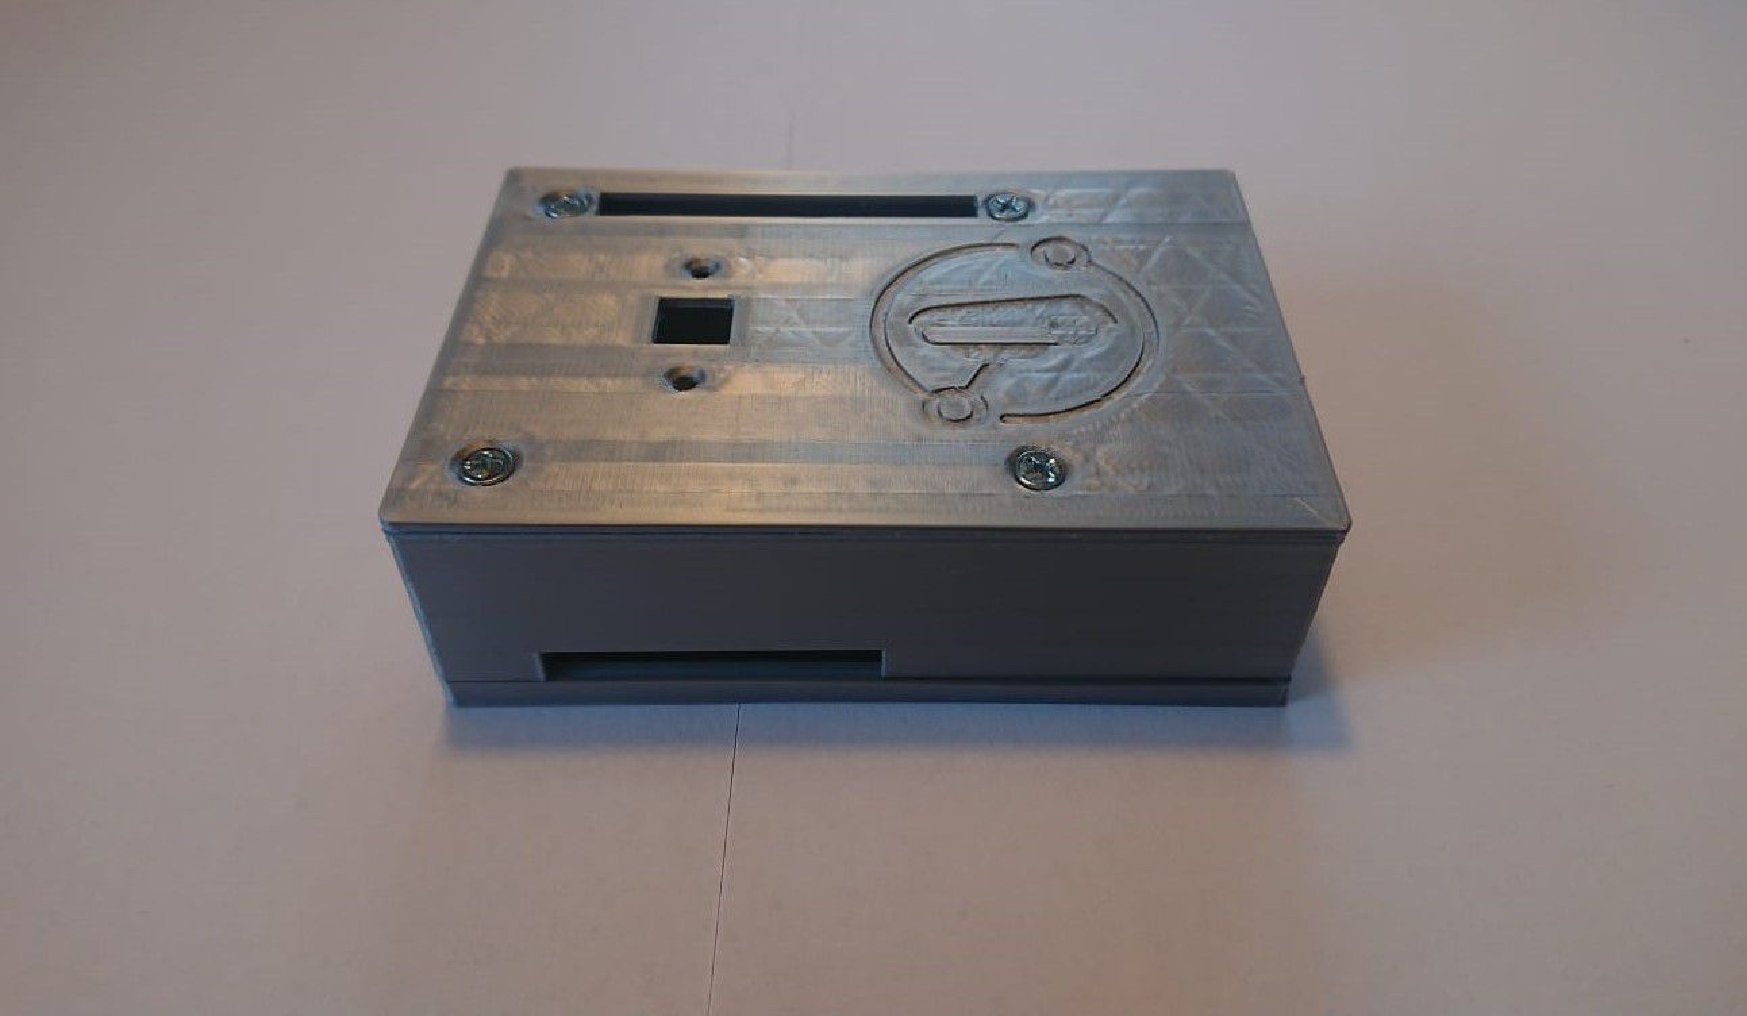
\includegraphics[width=0.8\linewidth]{kennzeichenerkennung/gtogether.pdf}
    \caption{Gesamtesansicht des gedruckten Gehäuses}
\end{figure}

Das fertige Gehäuse erfüllt alle zu Beginn definierten Anforderungen und ist somit bestens für diese Anwendung geeignet.

\subsection{Test}

\subsubsection{Einleitung}
Um die Kennzeichenerkennung zu testen und herauszufinden wie genau sie in der Praxis ist, wurden mehrere Tests durchgeführt, welche aufschlussreiche Ergebnisse geliefert haben.
Für den Test wird als Stromversorgung eine Powerbank verwendet und ein Laptop wird mit dem Raspberry Pi über VNC\footnote{Virtual Network Computing} verbunden um die Ergebnisse auszuwerten.

\begin{figure}[H]
    \centering
    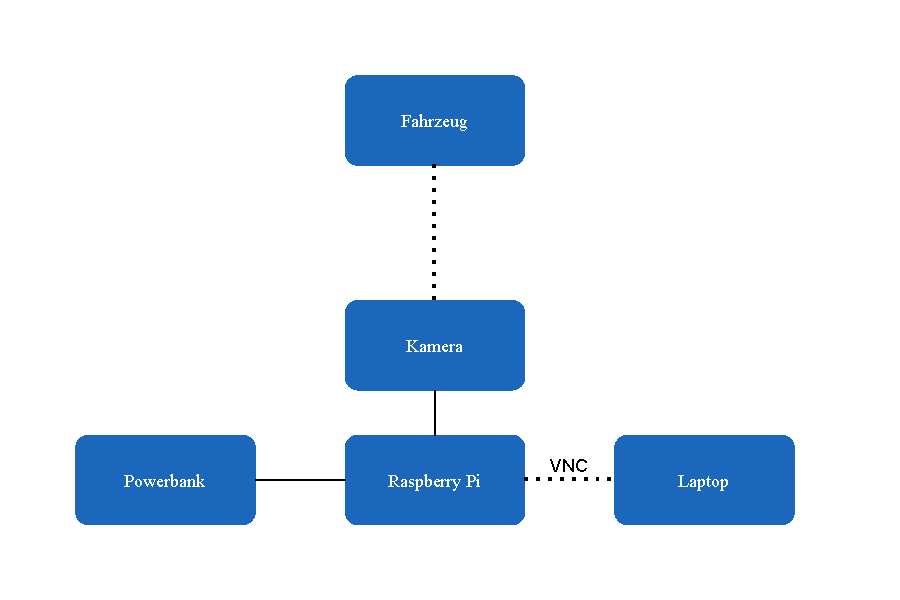
\includegraphics[width=0.9\linewidth]{kennzeichenerkennung/Testaufbau.pdf}
    \caption{Testaufbau}
\end{figure}

\subsubsection{Erster Test}
Im ersten Test wurde die Kennzeichenerkennung zum ersten Mal in der Praxis ausprobiert. Dies geschah in einer sehr schwierigen Umgebung mit schlechter Beleuchtung 
und vielen Lichtreflexionen durch Schnee. In der nachfolgenden Abbildung sieht man ein Bild dieses Tests.

\begin{figure}[H]
    \centering
    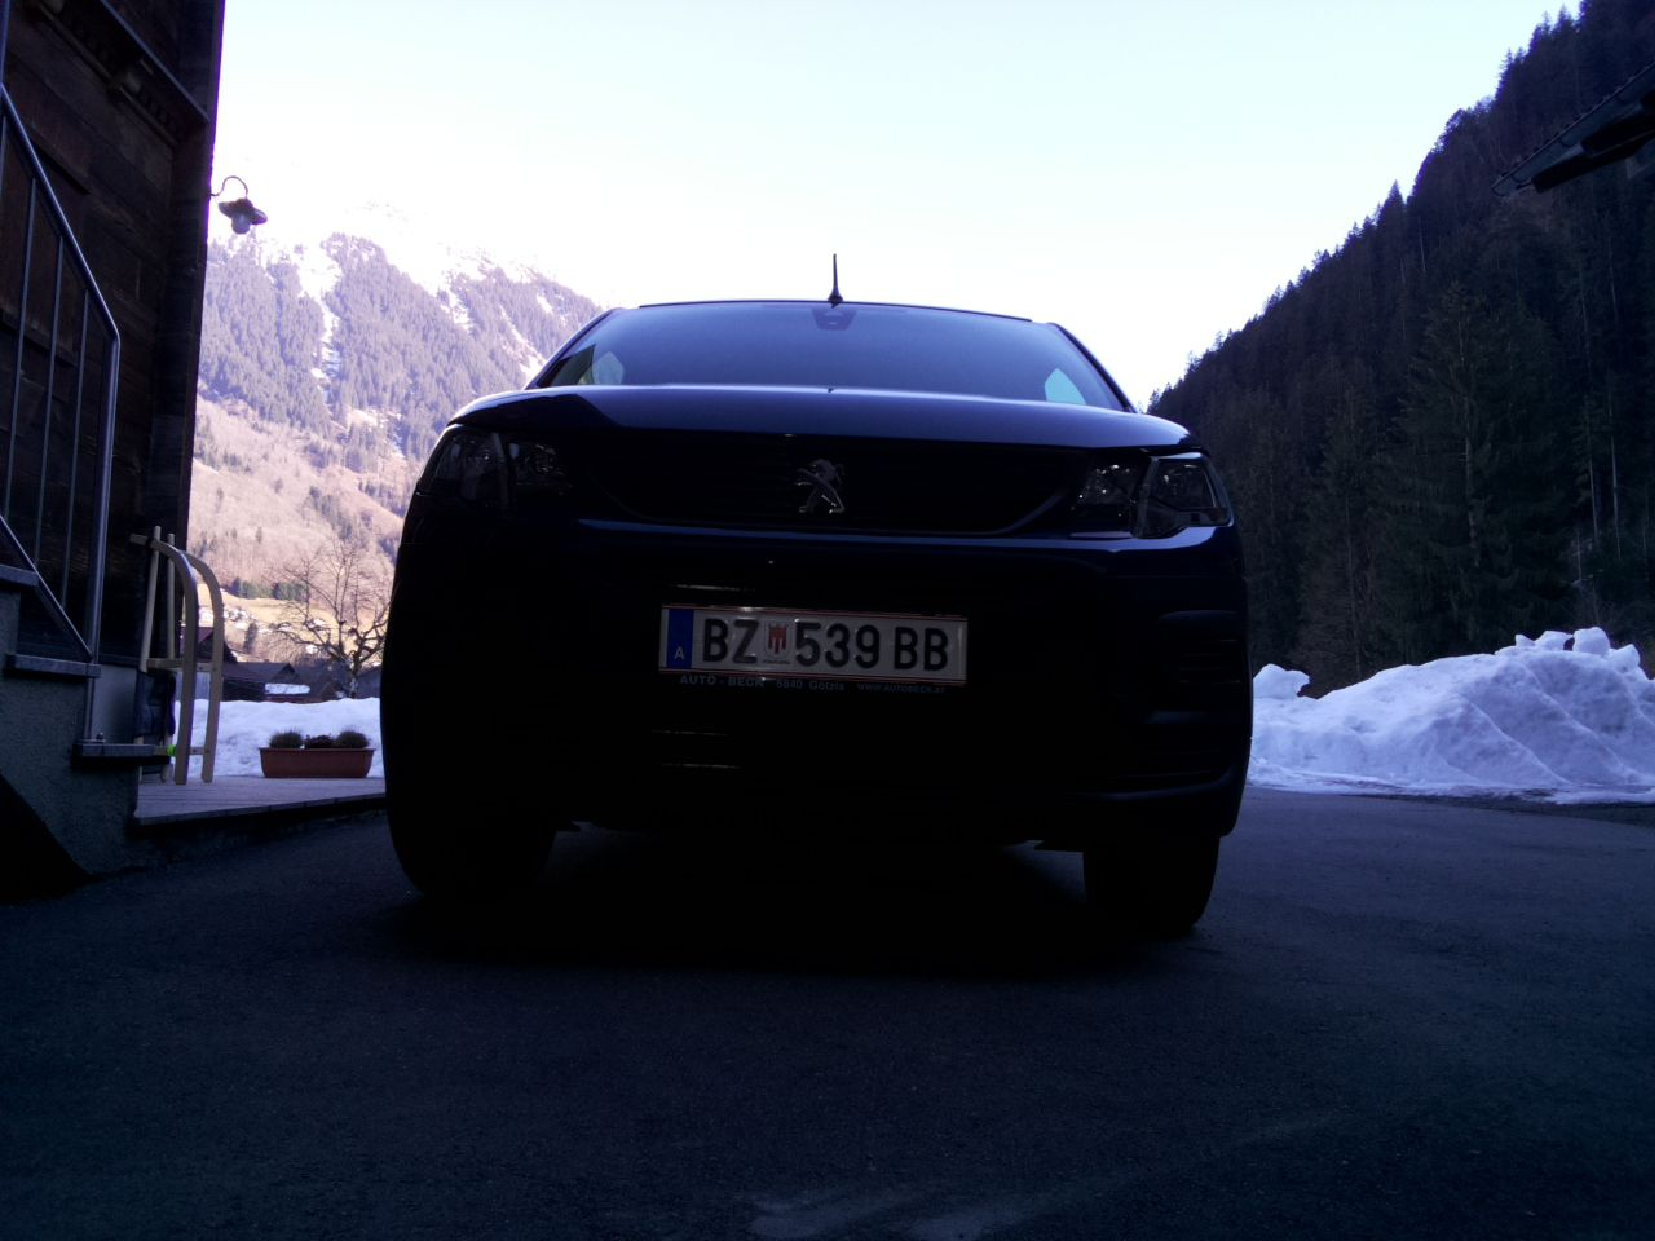
\includegraphics[width=0.8\linewidth]{kennzeichenerkennung/test1.pdf}
    \caption{Erster Test}
\end{figure}

Dieses Bild war eines der wenigen Bilder welches nicht durch Lichtreflexionen überbelichtet wurde, daran konnte man bemerken, dass die Kamera des Raspberry Pi eindeutig 
nicht für solche Verhältnisse geschaffen wurde, aber trotzdem keine allzu schlechten Ergebnisse liefert. Die Kennzeichenerkennung lieferte für dieses Bild das Ergebnis „82538BB“. 
Dies war kein schlechter erster Test, aber er zeigte, dass die Kennzeichenerkennung noch Schwierigkeiten mit der Unterscheidung von ähnlichen Zeichen wie zum Beispiel 
„8“ und „B“ oder auch „2“ und „Z“ hatte. Um dieses Problem zu lösen, wurde das Modell Training noch einmal überarbeitet, um die Genauigkeit der Zeichenerkennung zu verbessern. 
Dies führte zu einer signifikanten Verbesserung, welche im zweiten Test deutlich zu erkennen ist.

\subsubsection{Zweiter Test}
Der zweite Test fand unter besseren Licht- und Umgebungsbedingungen statt und zusätzlich wurde auch die Genauigkeit der Zeichenerkennung verbessert. 
Während des zweiten Tests wurde mit über 10 verschiedenen Fahrzeugen die Kennzeichenerkennung ausgetestet. Im Folgenden werden einige der unterschiedlichen Testbilder 
und deren Resultate gezeigt und analysiert.

\begin{figure}[H]
    \centering
    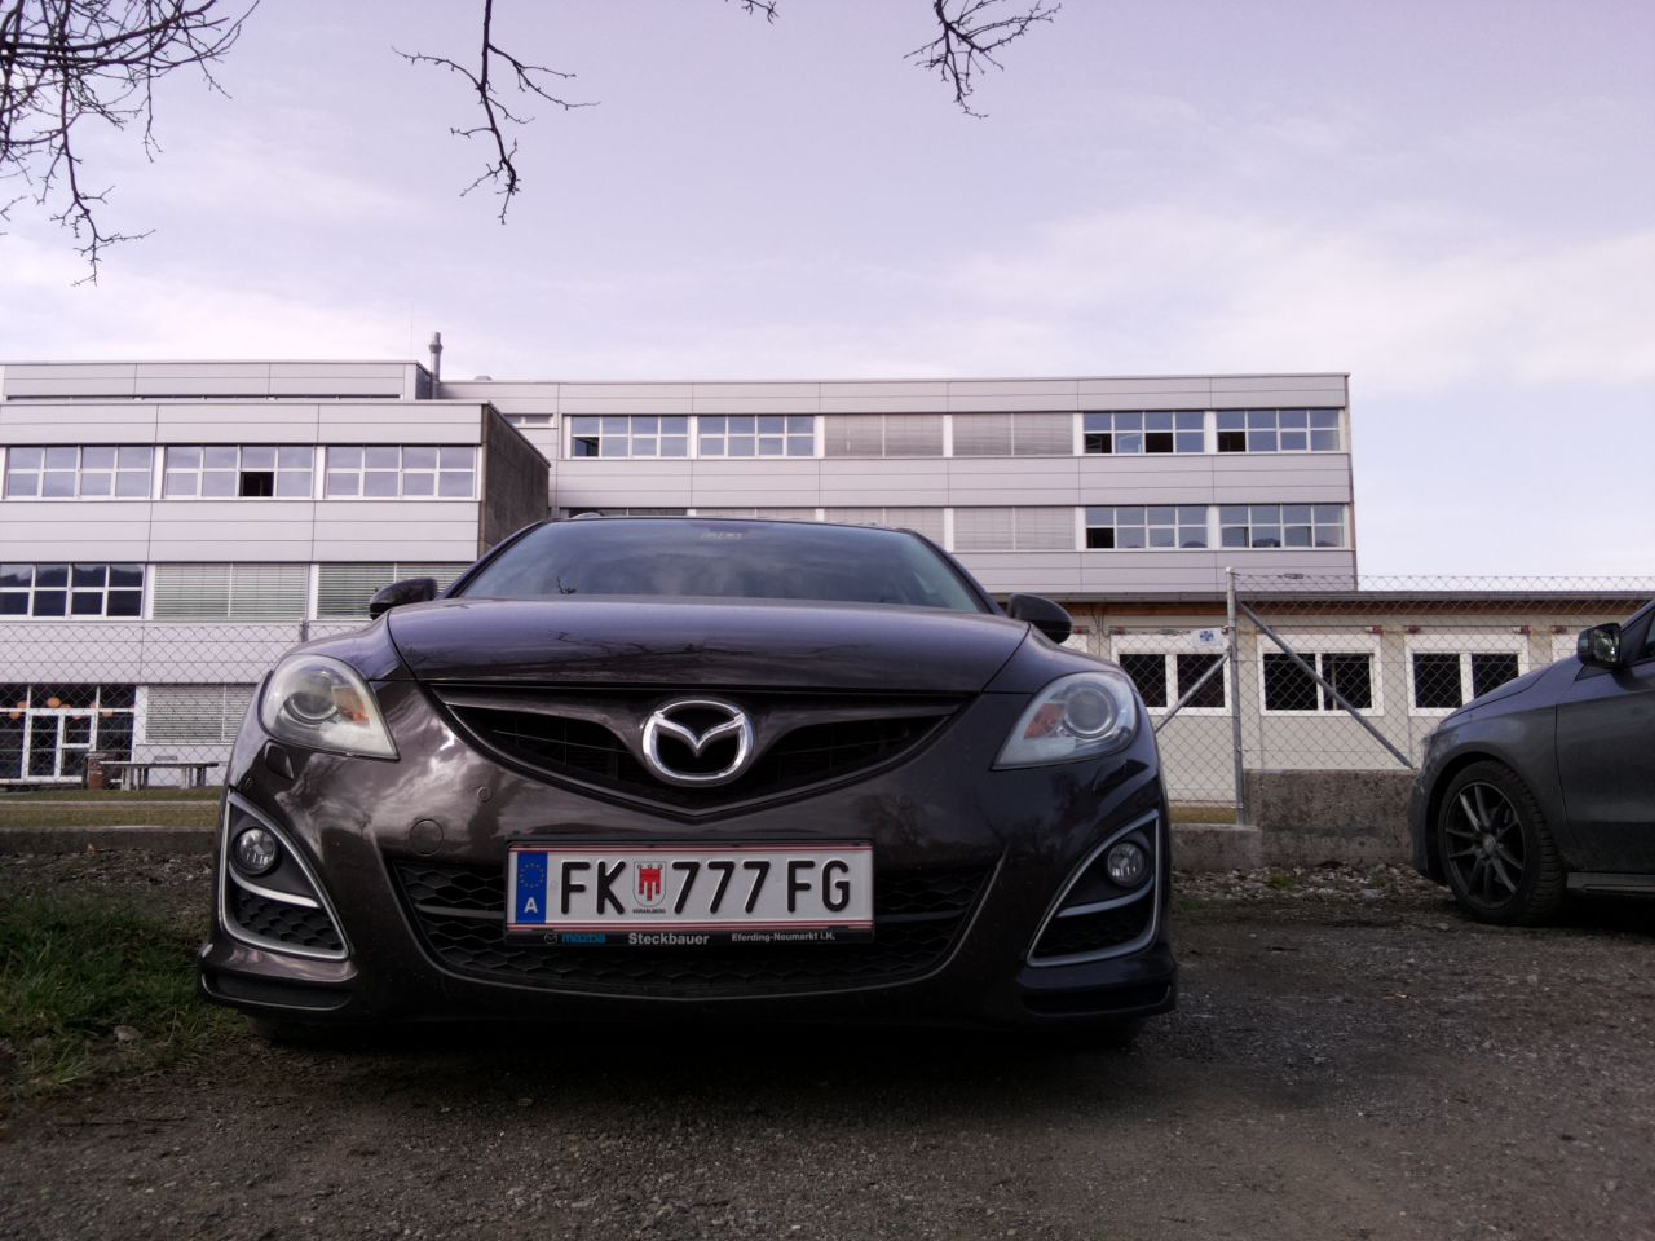
\includegraphics[width=0.8\linewidth]{kennzeichenerkennung/test2.pdf}
    \caption{Zweiter Test | Bild 1}
\end{figure}

\textbf{Resultat:} FK773FG\\

In diesem Bild wurde das Kennzeichen nahezu perfekt erkannt. Der einzige Unterschied liegt in der dritten „7“, welche vom Programm als „3“ erkannt wurde.

\begin{figure}[H]
    \centering
    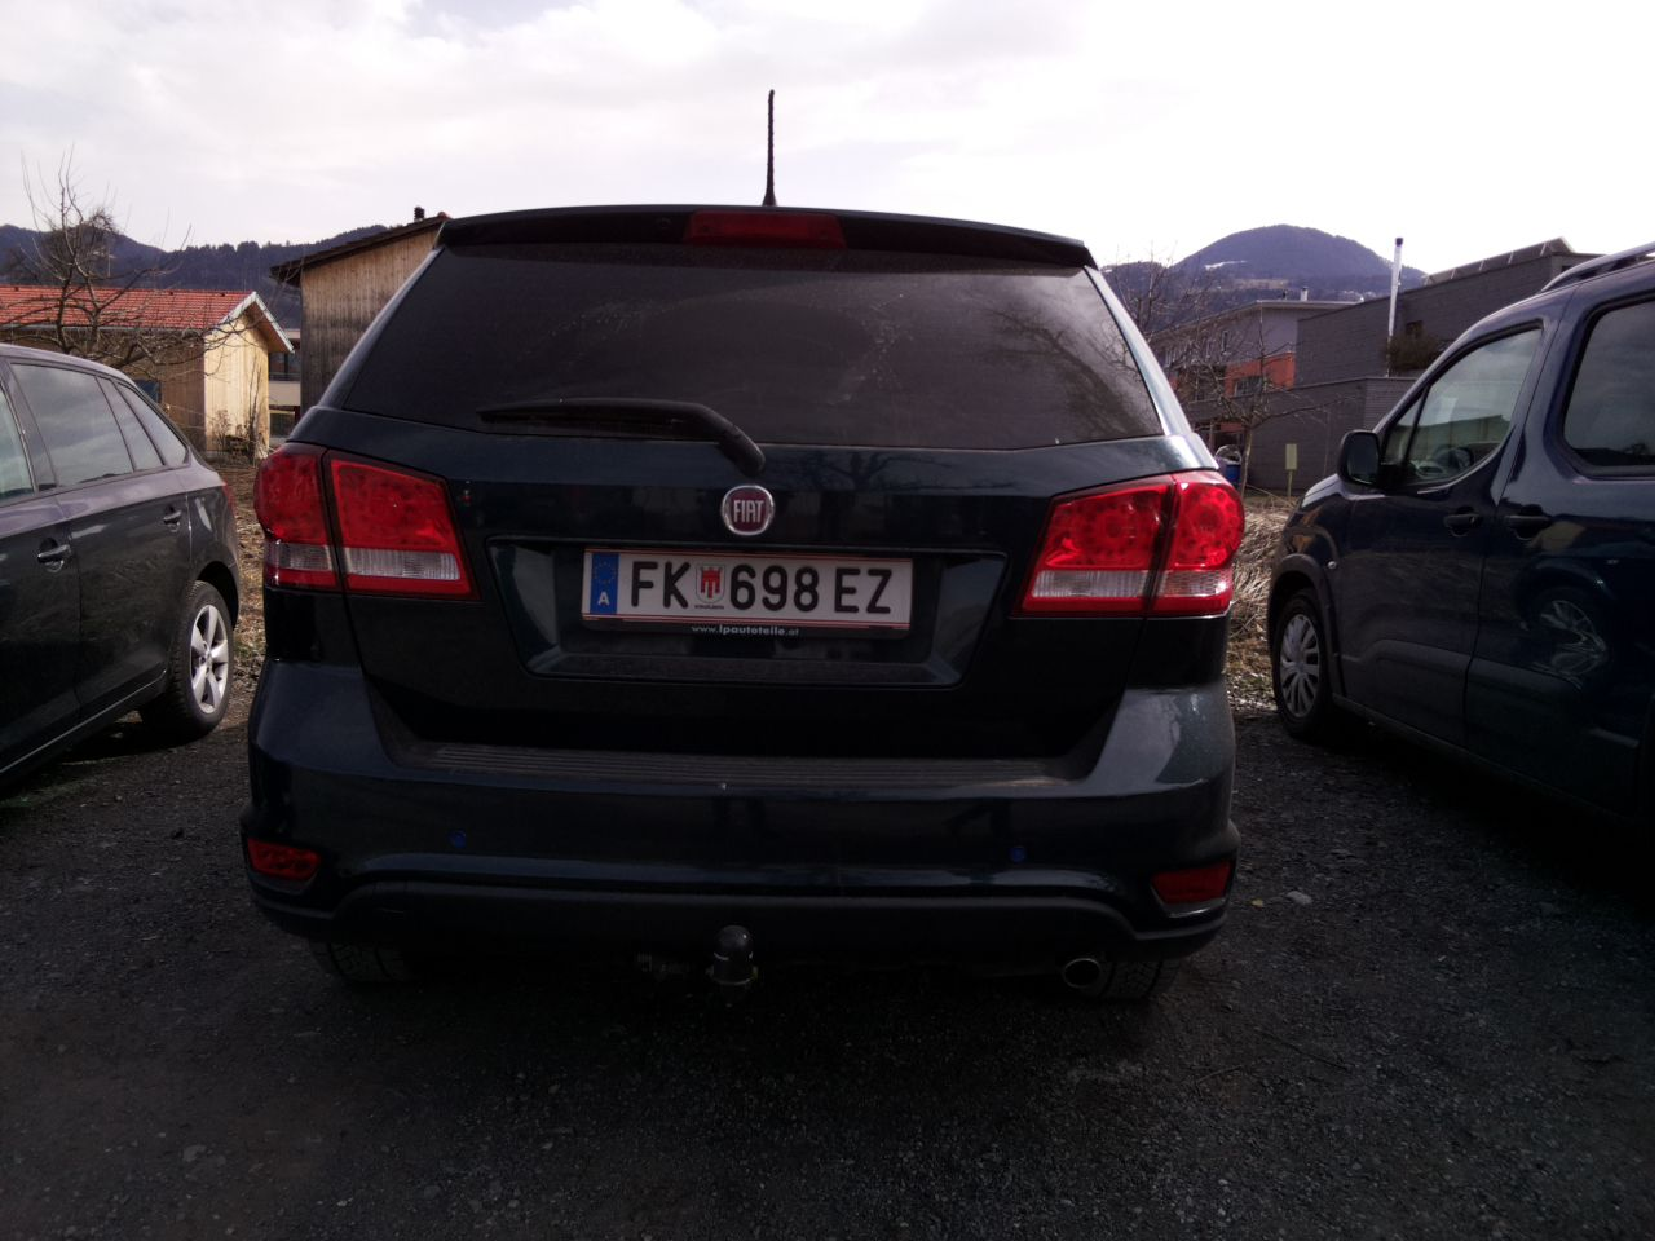
\includegraphics[width=0.8\linewidth]{kennzeichenerkennung/test3.pdf}
    \caption{Zweiter Test | Bild 2}
\end{figure}

\textbf{Resultat:} Nicht erkannt\\

Dieses Bild führte zu einem Fehler, weil in dem Bild kein Kennzeichen erkannt wurde. Dies kann zwei mögliche Ursachen haben. 
Entweder wurde von YOLOv2 im Bild kein Fahrzeug erkannt, oder es wurde von WPOD-NET kein Kennzeichen erkannt. Dies sind mögliche Fälle, da beide Modelle keine 
Genauigkeit von 100\% aufweisen.

\begin{figure}[H]
    \centering
    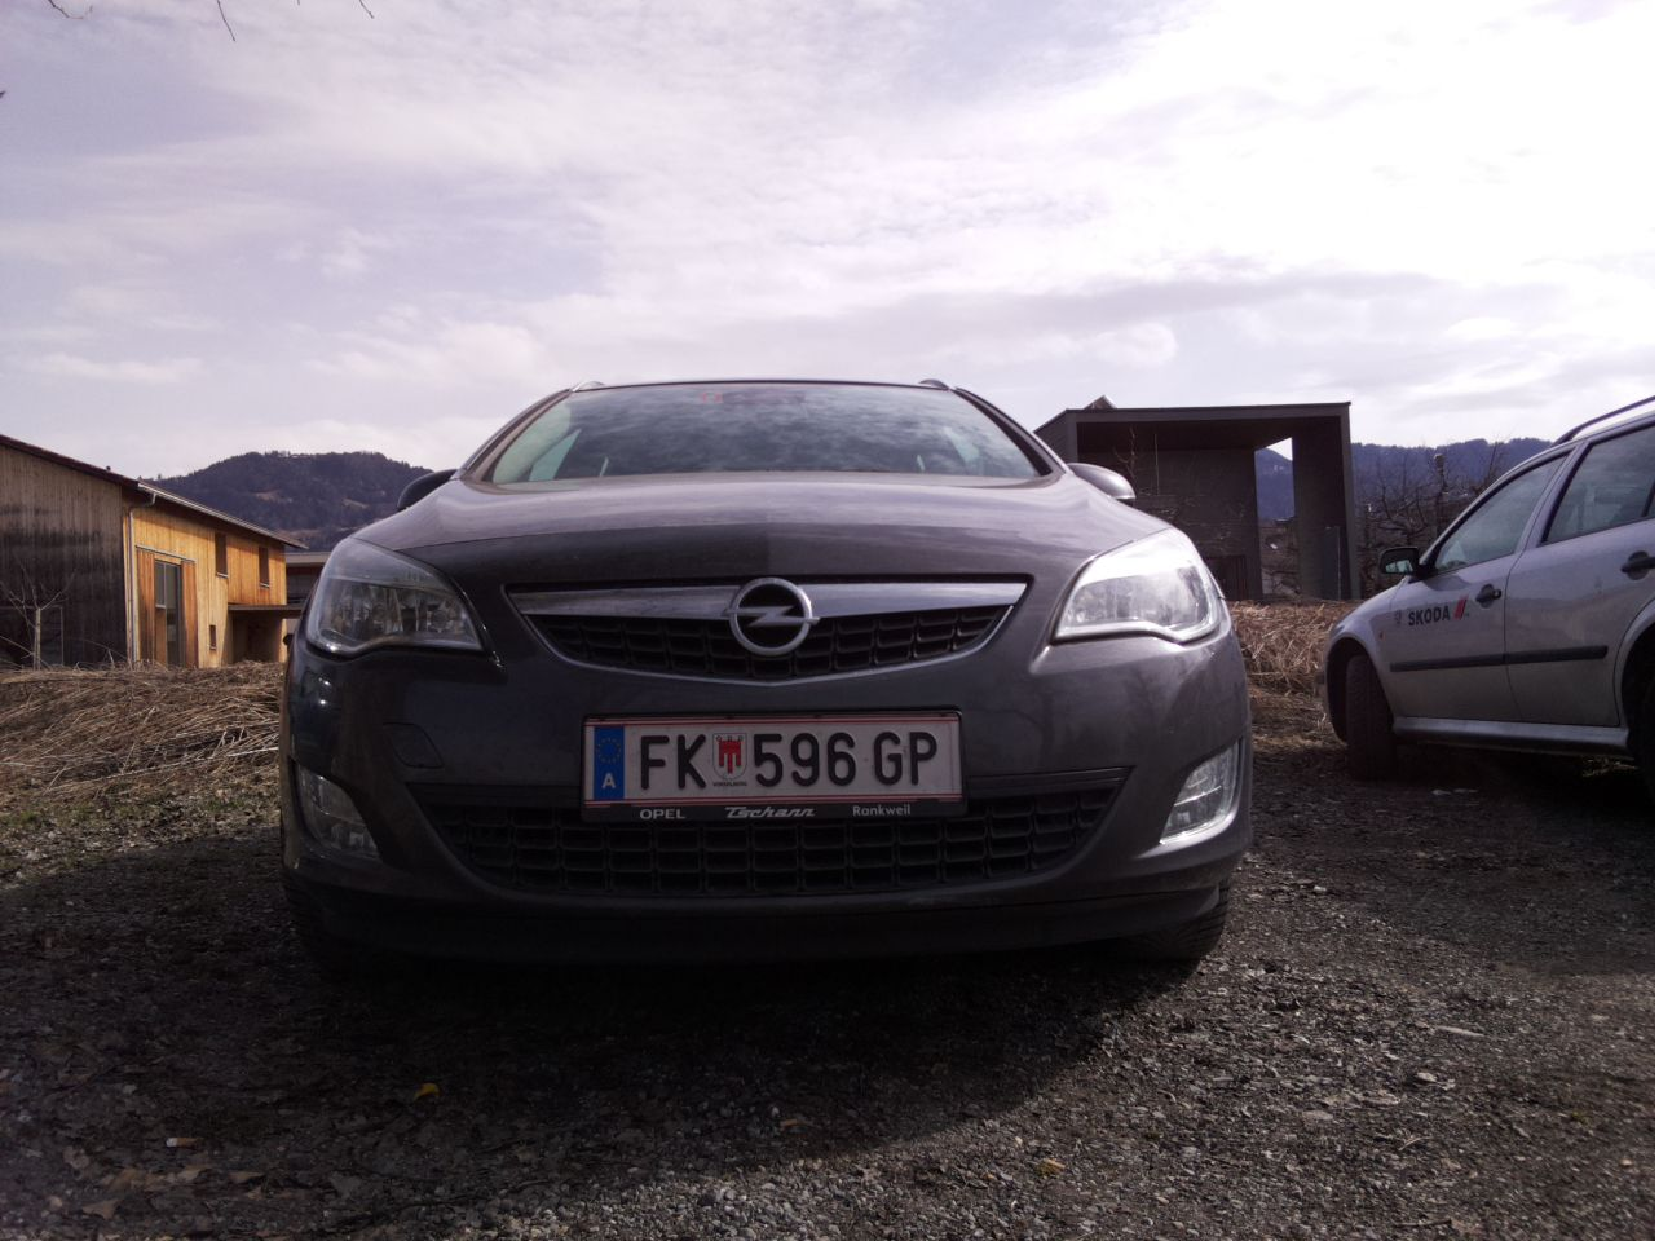
\includegraphics[width=0.8\linewidth]{kennzeichenerkennung/test4.pdf}
    \caption{Zweiter Test | Bild 3}
\end{figure}

\textbf{Resultat:} FK 596 GP\\

In diesem Bild wurde das Kennzeichen ohne jeglichen Fehler ausgelesen und die Kennzeichenerkennung hat damit einwandfrei funktioniert.

\begin{figure}[H]
    \centering
    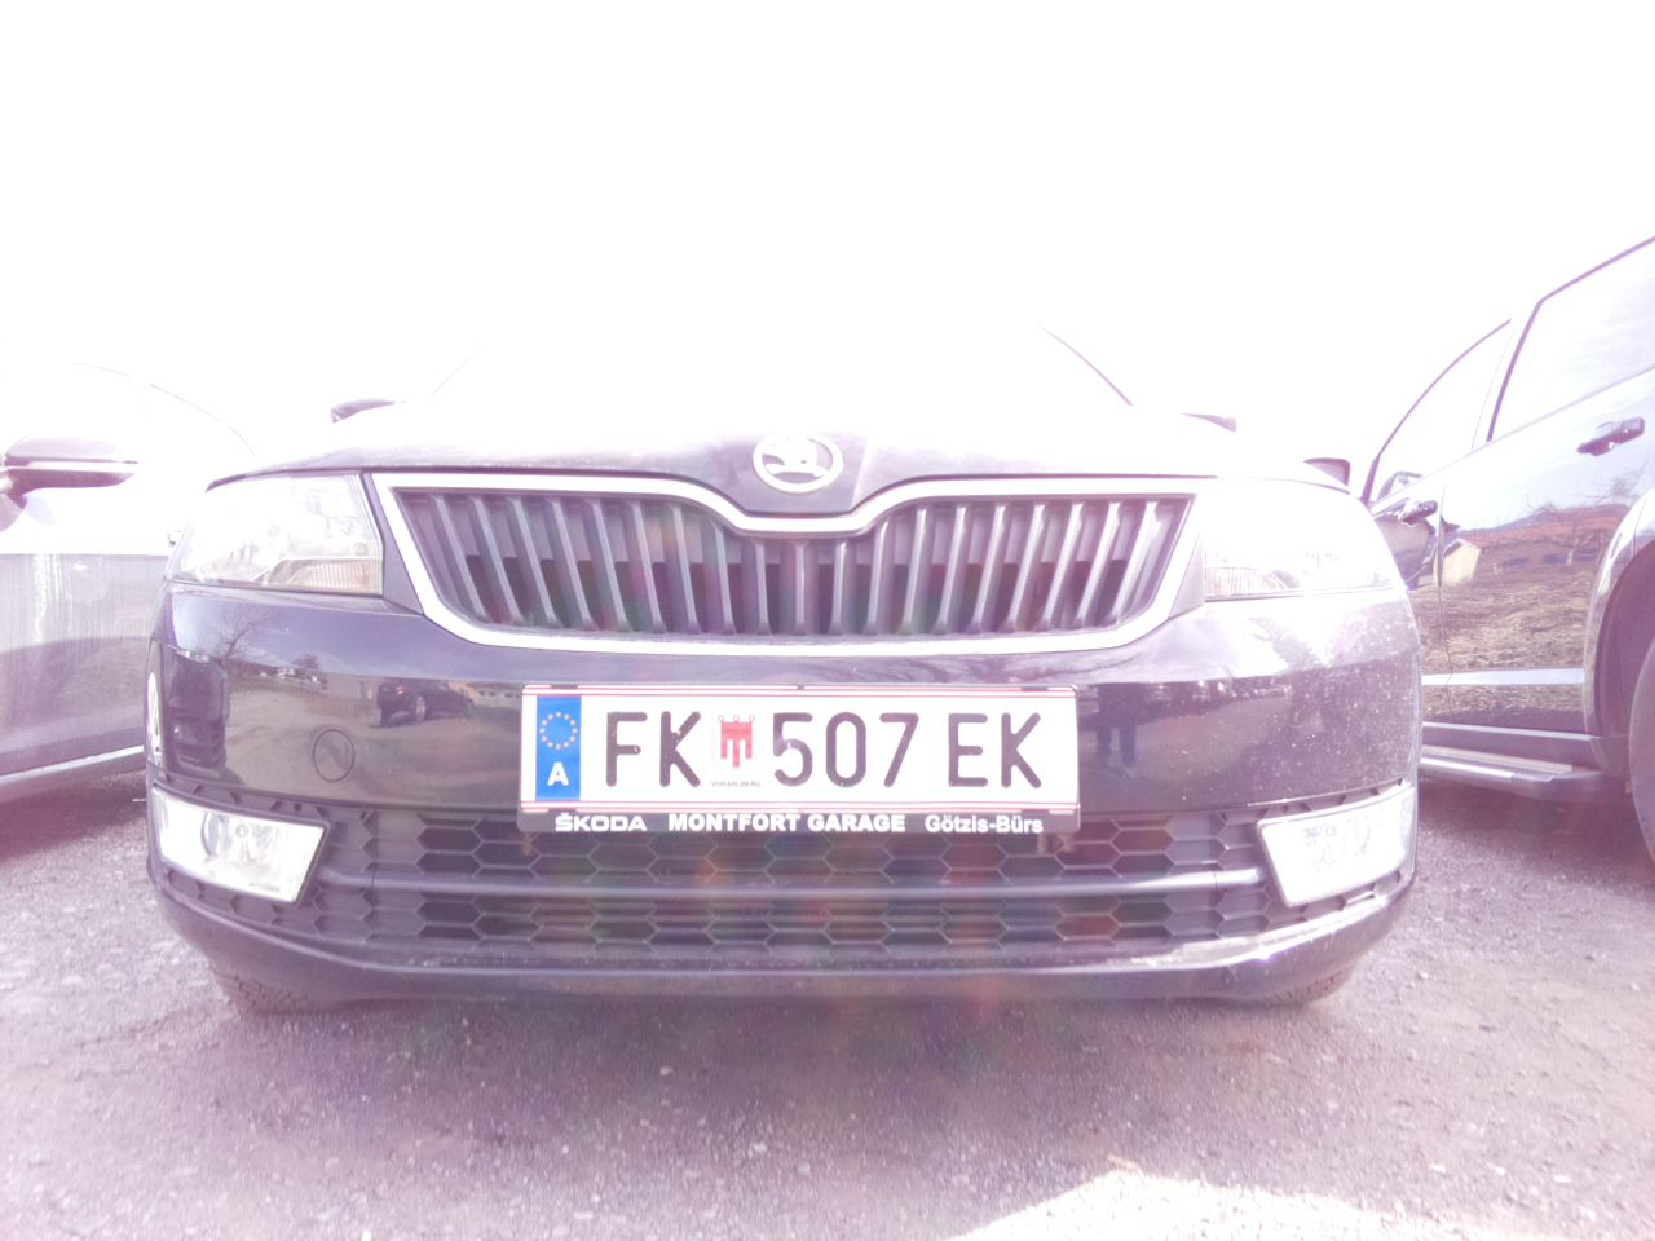
\includegraphics[width=0.8\linewidth]{kennzeichenerkennung/test5.pdf}
    \caption{Zweiter Test | Bild 4}
\end{figure}

\textbf{Resultat:} FK0K\\

Dieses Bild lieferte ein sehr interessantes Resultat. Wie im Bild eindeutig erkennbar ist, hat die Kamera das komplette Bild massiv überbelichtet, 
wodurch einiges sehr schlecht erkennbar ist. Trotz dieser erschwerten Bedingungen hat es die Kennzeichenerkennung aber geschafft einige der Zeichen 
korrekt auszulesen. Die anderen Zeichen wurden gar nicht erst erkannt, was auf die Zeichensegmentierung zurückzuführen ist.

\begin{figure}[H]
    \centering
    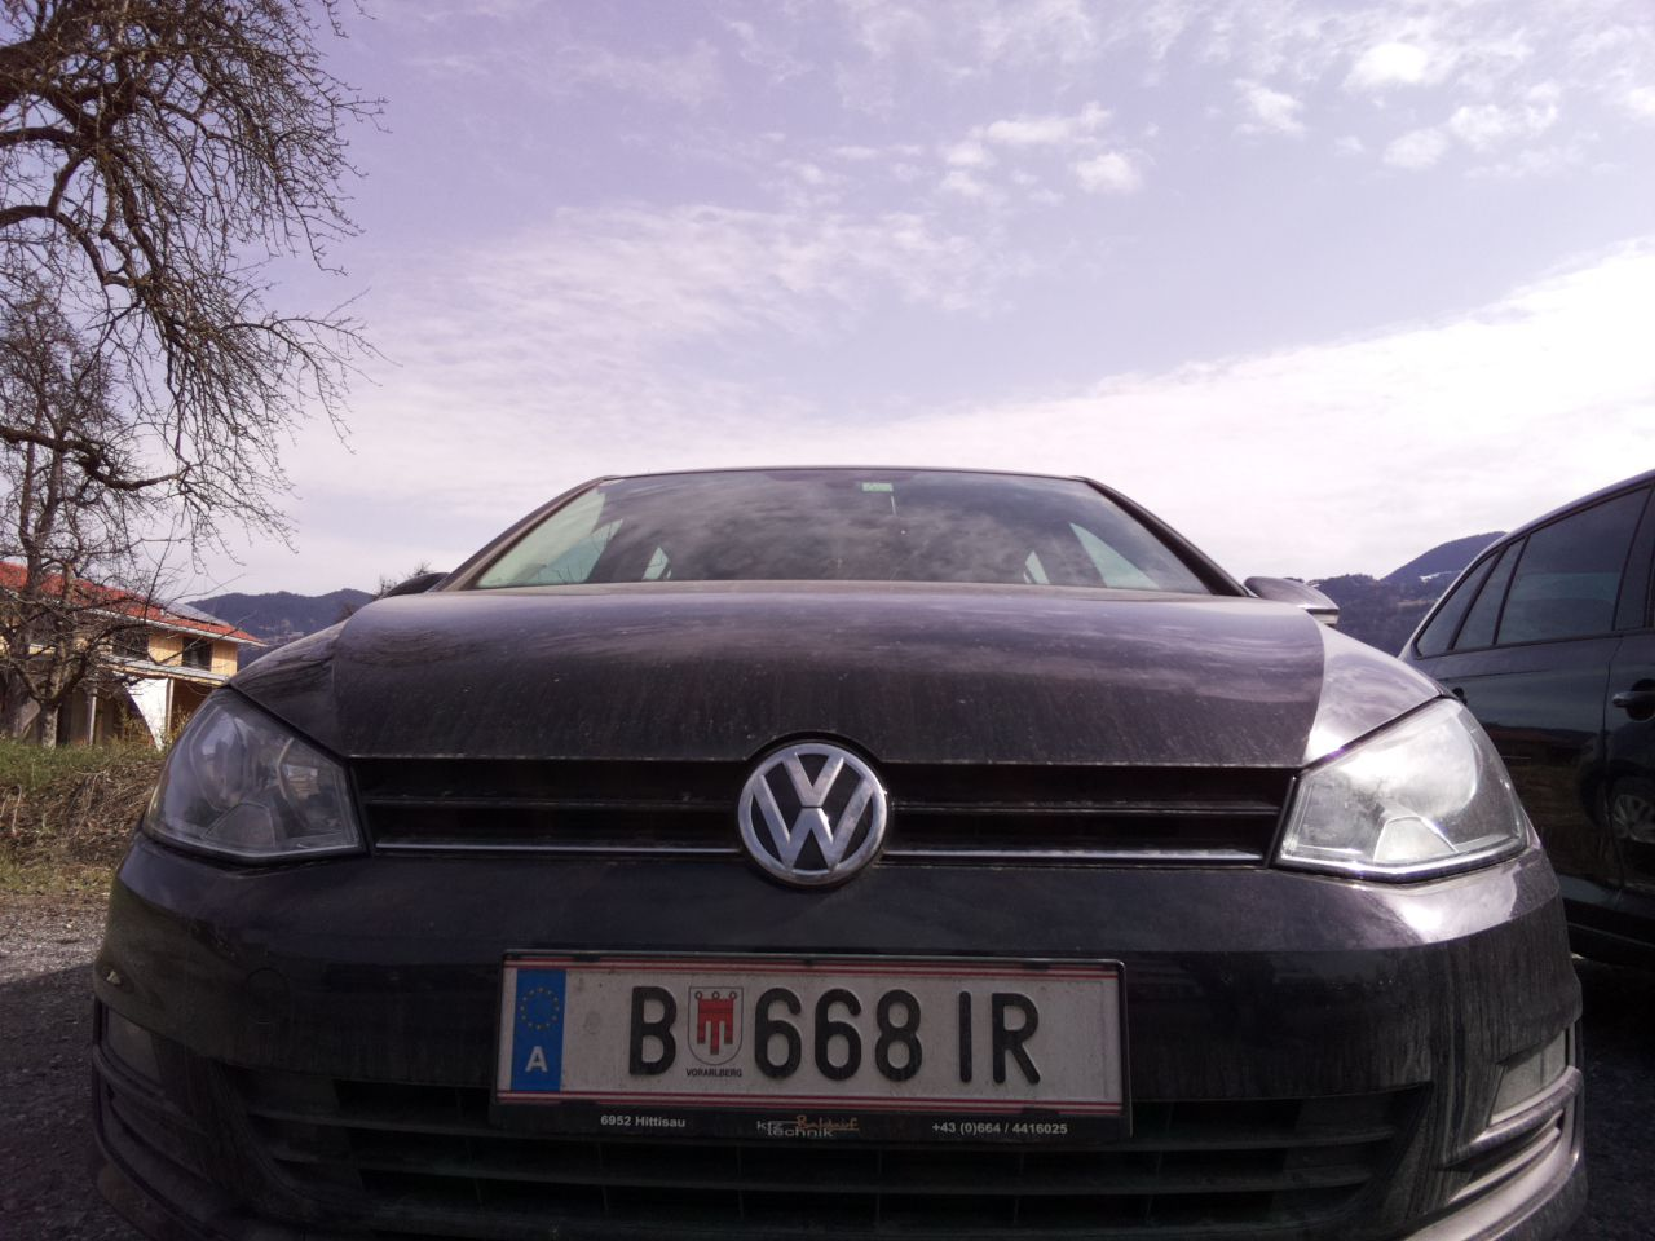
\includegraphics[width=0.8\linewidth]{kennzeichenerkennung/test6.pdf}
    \caption{Zweiter Test | Bild 5}
\end{figure}

\textbf{Resultat:} B668IR\\

Auch in diesem Bild wurde das Kennzeichen ohne jeglichen Fehler ausgelesen.

\subsubsection{Fazit}
In den Tests ist klar erkennbar, dass die Kennzeichenerkennung gute Resultate liefert. Vor allem die Steigerung der Genauigkeit vom ersten zum zweiten 
Test ist dabei hervorzuheben. Die berechnete Genauigkeit von etwa 87\% für eine fehlerfreie Kennzeichenerkennung konnte mit dem zweiten Test durchaus bestätigt werden. 
Die größte Schwachstelle der Kennzeichenerkennung ist jedoch die Kamera, welche sehr sensibel auf die unterschiedlichen Lichtverhältnisse reagiert. 
Ansonsten hat die Kennzeichenerkennung nahezu alle Kennzeichen fehlerfrei ausgelesen und nur ein einziges Kennzeichen wurde nicht erkannt. 
\pagebreak


\section{Fahrzeugerkennung}
\def \sectionauthors {Dennis Köb}
\subsection{Anforderungen}
Das Ziel der Fahrzeugerkennung ist es Fahrzeuge auf mehrere Parklücken eines Parkplatzes zu erkennen. Die daraus 
gewonnen Zustände sollen an das Webinterface übermittelt und an den jeweilige Parklücken über LEDs ausgegeben werden. 
\subsection{Vorstudie}

\subsection{Erkennung von Metallen über Spulen}
Grundsätzlich werden in der Realität häufig Spulen verwendet, welche unter dem Asphalt verbaut sind, um darüberliegende
Fahrzeuge zu detektieren. Als Messprinzip wird die Änderung des magnetischen Widerstands $R_{m}$ bei konstanter magnetischer Spannung $U_{m}$ und
daraus resultierende magnetischen Fluss $\phi$
Es gelten für diese Größen der folgende Zusammenhänge:

\begin{equation} \label{eq:phi}
    \Phi = \frac{U_{m}}{R_{m}}
\end{equation}

Wobei \\
$\Phi$ = magnetischer Fluss \\
$R_{m}$ = magnetischer Widerstand \\
$U_{m}$ = magnetische Spannung
\pagebreak

Der magnetische Widerstand lässt sich wiederum durch die Eigneschaften der Spule bestimmen. Die Formel hierfür lautet:

\begin{equation} \label{eq:Rm}
    R_{m} = \frac{N \cdot (2a + 2b)}{\mu_{0} \cdot \mu_{r} \cdot A} 
\end{equation}


Wobei \\
\begin{equation} \label{eq:A}
    A = a \cdot b
\end{equation}
$N$ = Anzahl der Windungen der Spule \\
$a$ = Breite der Spule in m \\
$b$ = Länge der Spule in m\\
$\mu_{0}$ = \SI[per-mode = symbol]{1.2566e-6}{\newton\per\ampere\squared} = magnetische Feldkonstante \\
$\mu_{r}$ = relative Permeabilität  \\
$A$ = Fläche der Spule

Bis auf die relative Permeabilität sind alle alle anderen Variablen konstant. Daraus lässt sich schlussfolgern, dass der magnetische
Fluss $\Phi$ anhand der Gleichung \ref{eq:phi} und \ref{eq:Rm} proportional zur relativen Permeabilität ist. 

\begin{equation} \label{iq:phi}
    \Phi \propto \mu_{r}
\end{equation}
Der Fluss $\Phi$ hängt somit auch von den Materialien ab durch die er fließt. In der nächsten Abbildung kann man erkennen,
wie ein Fahrzeug über eine im Boden installierte Spule den magnetischen Fluss $\Phi$ und somit die magnetische Flussdichte $B$
beeinflussen kann. 

\begin{figure}[H]
    \centering
    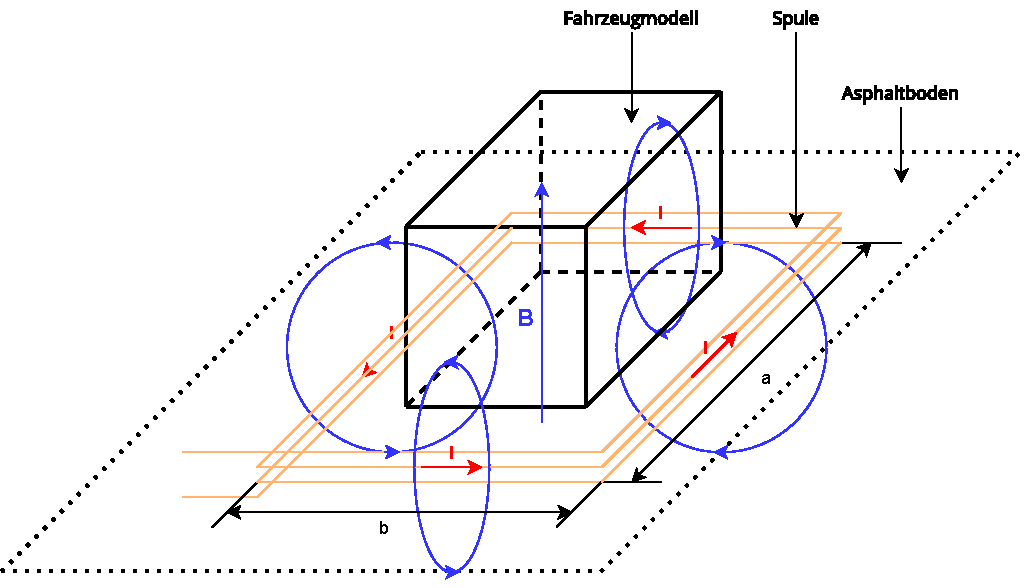
\includegraphics[width=1\linewidth]{fahrzeugerkennung/Spuleninstallation.pdf}
    \caption{Installation der Spule}
  \end{figure}
Um diese Größen auslesbar zu machen, müssen diese magnetischen bei einer direkten Messung in elektrische Größen umgewandelt
werden.
Hierfür gelten folgende Zusammenhänge:

\begin{equation} \label{eq:L_phi}
    L = \frac{N \cdot \Phi}{I} = \frac{\Psi}{I} 
\end{equation}
Wobei \\
$L$ = Induktivität der Spule \\
$I$ = Strom der durch die Spule fließt \\
$N$ = Anzahl der Windungen der Spule \\
$\Psi$ = Verkettete Fluss

\pagebreak
\begin{equation} \label{eq:L_i}
    u(t) = L \cdot \frac{di(t)}{dt}
\end{equation}

Wobei \\
$L$ = Induktivität der Spule \\
$i(t)$ = Strom der durch die Spule fließt zum Zeitpunkt t \\
$u(t)$ = Spannung die an der Spule anliegt zum Zeitpunkt t \\
$t$ = Zeit in s \\
So lässt sich bei Bekanntheit von Strom und Spannung auf die Induktivität und mit der Gleichung \ref{eq:L_phi} 
und mit den Zusammenhang \ref{iq:phi} auf die magnetischen Eigenschaften des Materials rückschließen. 
Diese Art der Detektion bietet viele praktische Vorteile.

\begin{itemize}
    \item \textbf{Größerer Messbereich} \\
    Im Vergleich zu anderen Detektionsmethoden wie einer Leichtschranke kann man einen größeren Bereich durch die Wirkfläche
    der Spule abdecken. So lassen sich auch kleinere Kraftfahrzeuge wie Motorräder oder Mopeds besser erkennen.
    \item \textbf{Schutz vor Umweltfaktoren} \\
    Durch den Verbau im Boden ist die Messeinrichtung vor Umwelteinflüssen wie Regen, Frost, hohen beziehungsweise
    niedrigen Temperaturen und Korrosion besser geschütz. Dies verringert auch den Einfluss dieser Störfaktoren auf die Eigenschaften
    Spule und somit auf die daraus resultierenden Messergebnisse.
    \item \textbf{Ausschließung von Materialien} \\
    Alle nicht metallische Stoffe werden von diesem Messprinzip nicht wahrgenommen. So können Verschmutzungen wie Blätter und Staub, welche
    visuelle Sensoren stören können, die Detektion nicht behindern.
    
\end{itemize}
\subsubsection{Messung ferromagnetischer Metalle}
Um diese Dtektionsverfahren zu verstehen muss zuerst der Zusammenhang zwischen Induktivität und relativer Permeabilität verstanden werden.
Aus den Gleichungen \ref{eq:Rm}, \ref{eq:phi} und \ref{eq:L_phi} kann die folgende Proportionalität ermittelt werden:
\begin{equation} \label{iq:L_mu}
    L \propto \mu_{r}
\end{equation}
Bei ferromagnetischen Stoffen wie Eisen ist die relative Permeabilität sehr viel größer als 1. Wenn nun ein Auto oder 
eine anderes Vehikel sehr viel Eisen beinhaltet wirkt sich die dies steigernd auf die Induktivität der Spule aus. Die folgenden
Verfahren nutzen dieses Prinzip um die Belegung einer Parklücke zu bestimmen.

\paragraph{RL-Oszillator mit Timer Baustein}\mbox{}\\
Bei diesem Messverfahren wird die Änderung der Induktivität $L$ über die Änderung einer Stromladekurve über einen Widerstand
$R$ ermittelt. Eine Simulation in LTSPice mit folgendem Schaltbild kann die Auswirkung auf eine Ladekurve bei gleicher Spannung
und gleichem Widerstand gut darstellen.
\begin{figure}[H]
    \centering
    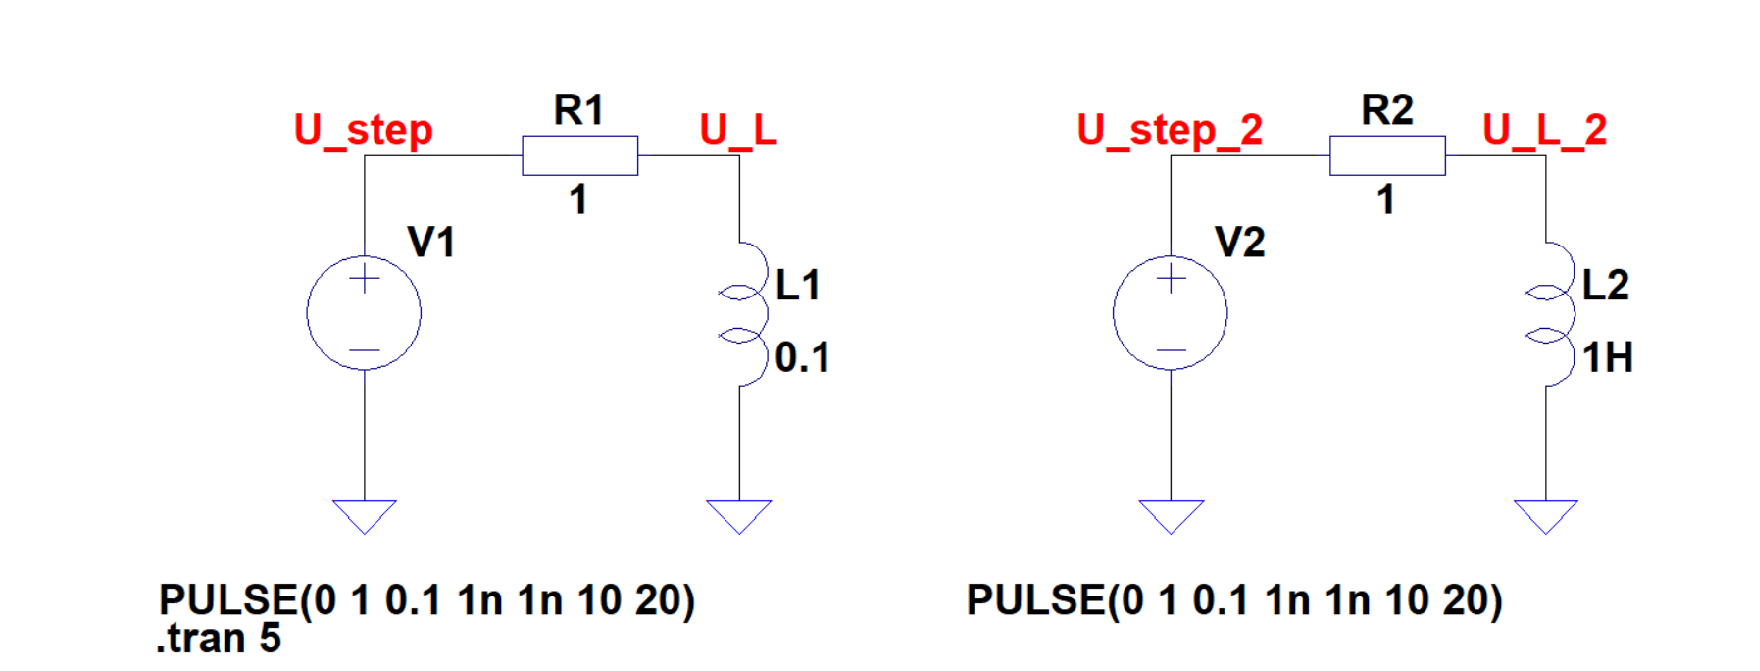
\includegraphics[width=1\linewidth]{fahrzeugerkennung/Ladekurven.pdf}
    \caption{LTSPice Blockbild zweier RL-Glieder}
\end{figure}
\pagebreak
Die daraus Resultierende Simulation im Zeitbereich ergibt folgendes Ergebnis:
hmm

\begin{figure}[H]
    \centering
    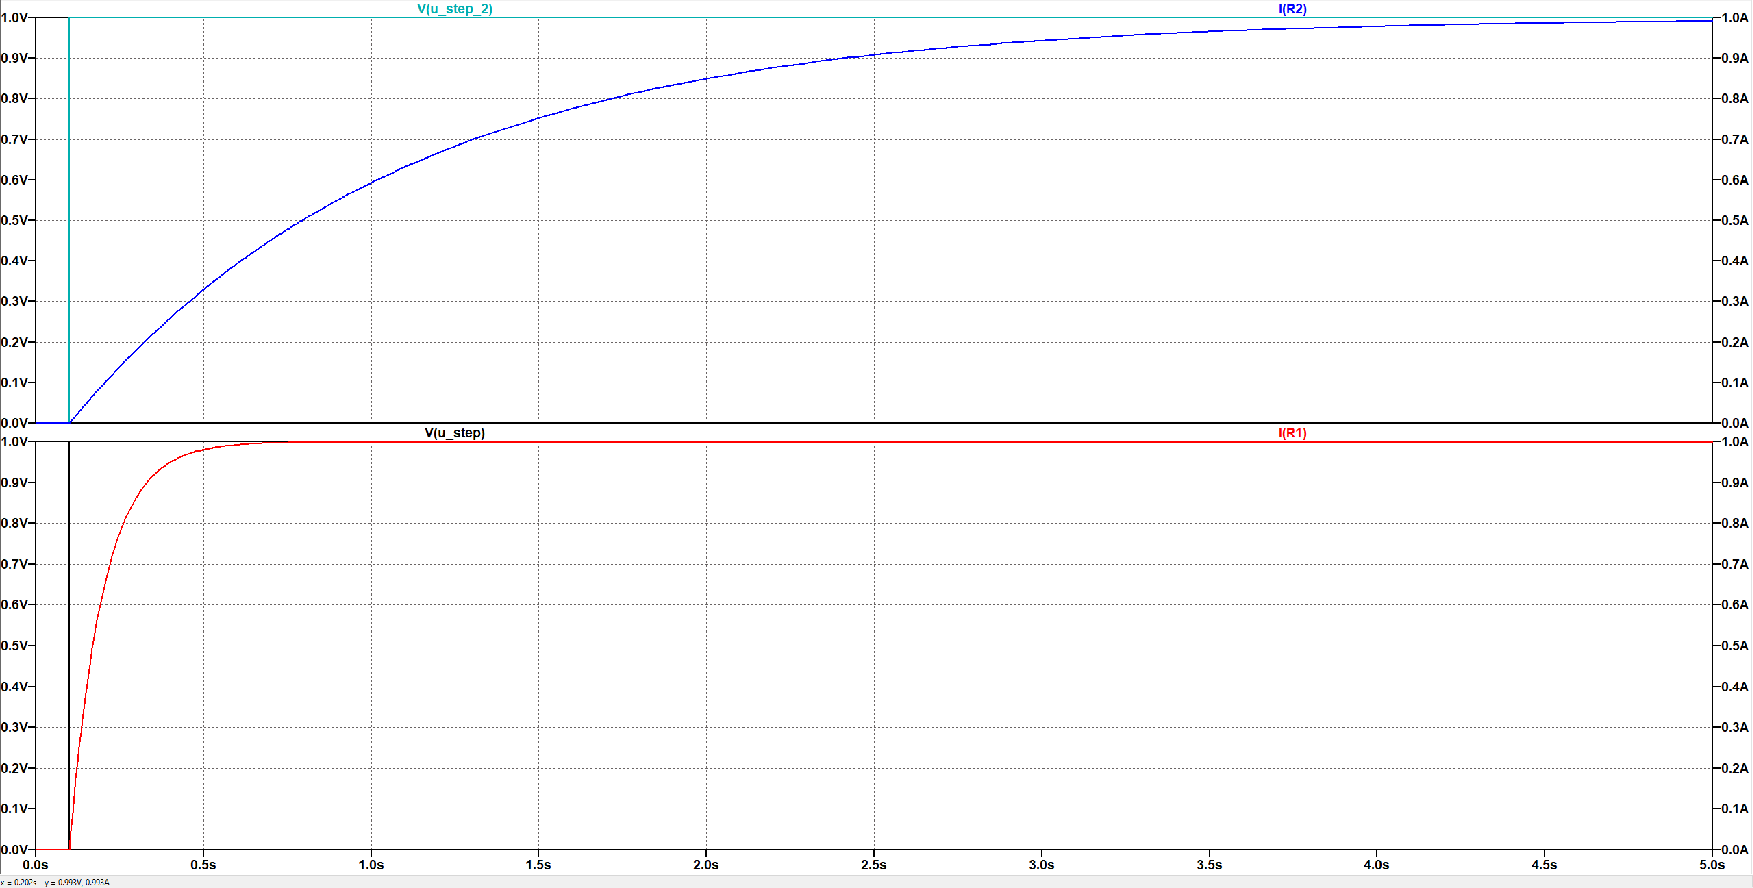
\includegraphics[width=1\linewidth]{fahrzeugerkennung/Ladekurven_ZB.pdf}
    \caption{Stromkurven zweier RL-Glieder}
\end{figure}

Es ist aus der letzten Abbildung erkennbar, dass sich eine größere Induktivität verlangsamend auf die Zunahme des Stromes auswirkt. Für Einschaltvorgänge kann diese Stromkurve
für RL-Glieder folgendermaßen beschrieben werden.

\begin{equation} \label{eq:i_L}
    i(t) = \frac{U_{0}}{R} \cdot (1 - e^{-\frac{t}{\tau}})
\end{equation}

\begin{equation} \label{eq:tau_RL}
    \tau = \frac{L}{R}
\end{equation} 

Wobei \\
$i(t)$ = Strom der durch die Spule fließt zum Zeitpunkt t \\
$L$ = Induktivität der Spule in H\\
$R$ = Widerstand in $\Omega$ \\
$U_0$ = Spannung die nach dem einschalten anliegt in V\\
$t$ = Zeit in s \\
$\tau$ = Zeitkonstante in $\frac{1}{s}$\\

Timer Bausteine wie der NE555 nutzen diese solche Verlaufskurven wenn sie als astabile Kippstufe konfiguriert sind.
Es gibt einen Eingang dieses Baustein meist CV für Control Voltage der die Spannung überwacht. Überschreitet diese Spannung zweit drittel
der Betriebsspannung schaltet er einen weiteren Pin, meist DIS für Discharge, auf 0V beziehungsweise auf Masse. Unterschreitet jedoch 
die Spannung am CV Pin ein drittel der Betriebsspannung so wird der DIS Pin auf Betriebsspannung geschalten. Diese beiden Pins 
sind über RC- oder RL- Glieder verbunden. Es entsteht somit ein Oszillator, welcher die Spannung am DIS Pin anhebt und absenkt.
Der NE555 kann dieses Signal über einen internen Komparator in ein Rechtecksignal umwandeln, welches besser von Mikrokontrollern ausgelesen
werden kann. Der Mikrokontroller kann so die Anzahl der ein einkommenden Takte über einen gewissen Zeitraum zählen und daraus eine Oszillatorfrequenz errechnen.
Die Zeitsignale lassen sich in LTSPice mit dem NE555 als Timer-Baustein simulieren.

\begin{figure}[H]
    \centering
    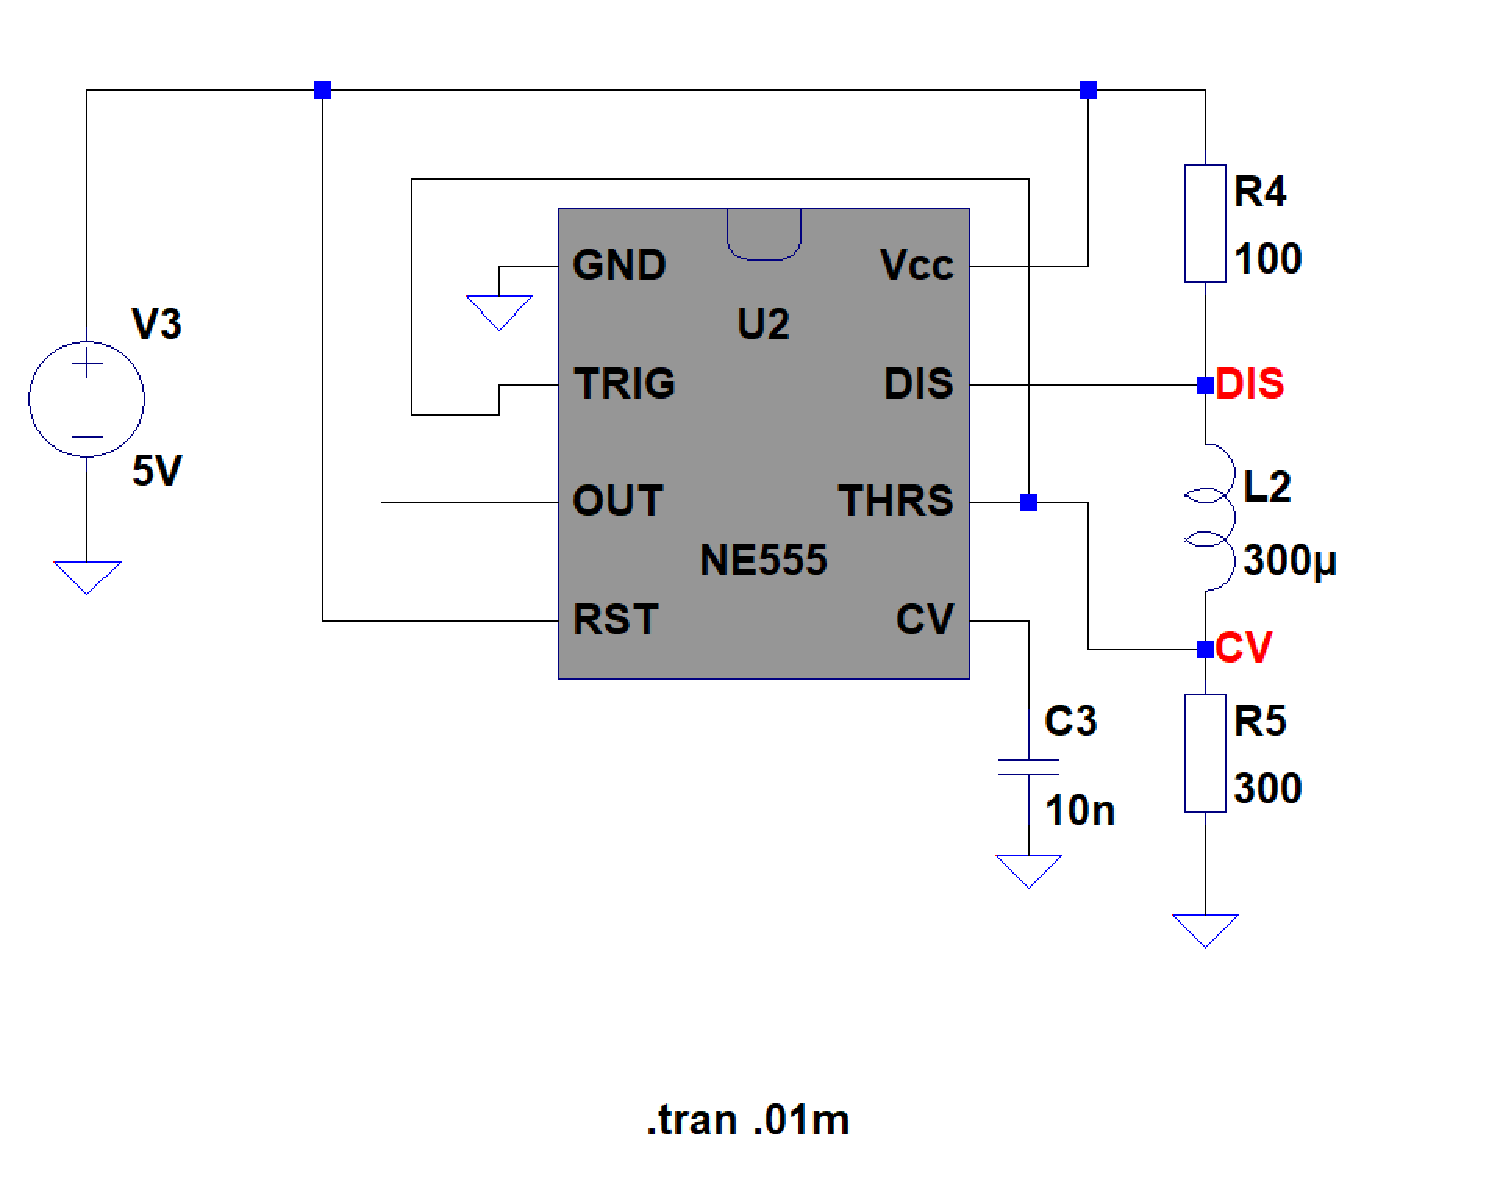
\includegraphics[width=0.6\linewidth]{fahrzeugerkennung/RL_Oszillator.pdf}
    \caption{RL-Oszillator mit NE555}
\end{figure}

\begin{figure}[H]
    \centering
    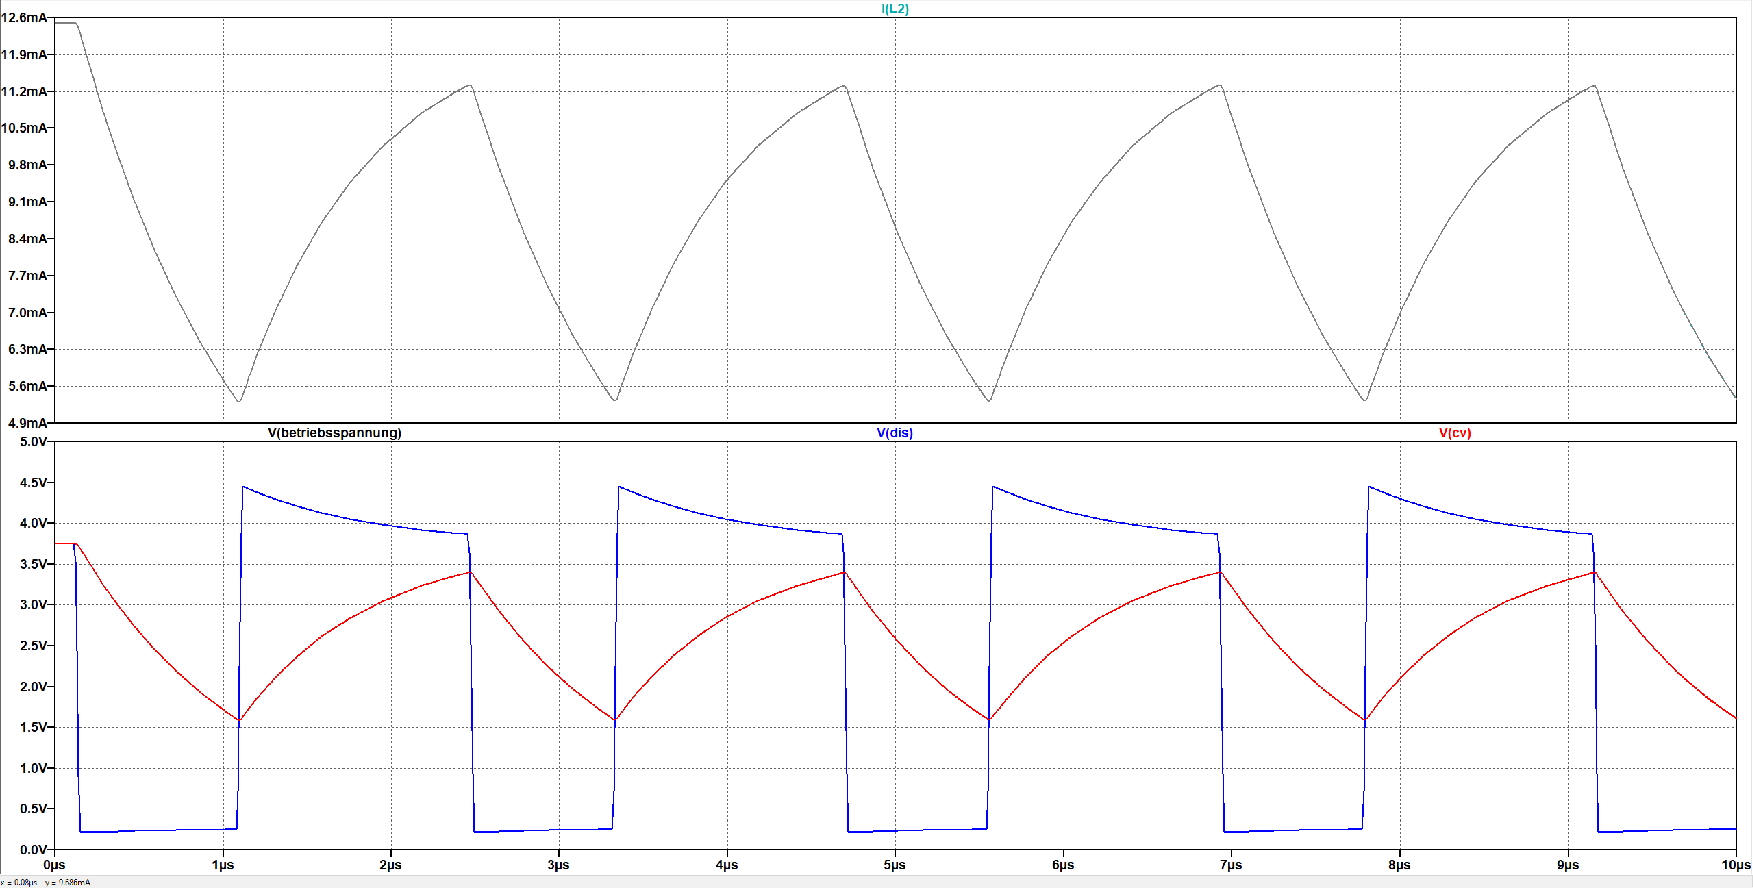
\includegraphics[width=1\linewidth]{fahrzeugerkennung/RL_Oszillator_ZB.pdf}
    \caption{RL-Oszillator mit NE555 Zeitsignale}
\end{figure}

Im oberen Diagramm ist der Verlauf des Stromes durch die Spule zu erkennen der wie erwartet zu- und abnimmt. Im unteren Diagramm ist in 
schwarz die Betriebsspannung als Referenz in rot der CV Pin und in blau der DIS Pin des NE555. Das rote Signal wechselt zwischen zwei drittel der Betriebsspannung 
und einem drittel der Betriebsspannung mit einer Frequenz von $f = \SI{438}{\kilo\hertz}$ bei einer Induktivität von $L = \SI{300}{\micro\henry}$, einem Widerstand $R4 = 100\Omega$ und einem
Widerstand $R5 = 300\Omega$. Die Simulation entspricht hier der Theorie, jedoch bricht das blaue Signal am PIN DIS in der Einschaltphase ein.
Der grund dafür ist der interne Widerstand des NE555, der ab einem gewissen Stromverbrauch für einen Spannungsabfall sorgt. Da es meist besser ist mit
niedrigen Frequenzen zu arbeiten ist es nach den Gleichungen \ref{eq:i_L} und \ref{eq:tau_RL} entweder nötig die Induktivität zu erhöhen oder die Widerstände zu verkleinern.
Die Induktivität lässt sich aber entweder durch erhöhen der Windungen oder durch Vergrößerung der Spule erreichen, was in vielen Fällen nicht möglich ist oder zunehmends kostspielig ist.
Die Reduktion der Widerstände führt zu einer Zunahme des Stromes und der Verlustleistung, was auch unerwünscht ist.
Aus diesen Gründen ist der RL-Oszillator nur für hohe Frequenzen geeignet. In der nächsten Abbildung sieht man die Schaltung bei verschiedene Induktivität
nämlich bei $L2 = \SI{100}{\micro\henry}$ und bei $L2 = \SI{1}{\milli\henry}$

\begin{figure}[H]
    \centering
    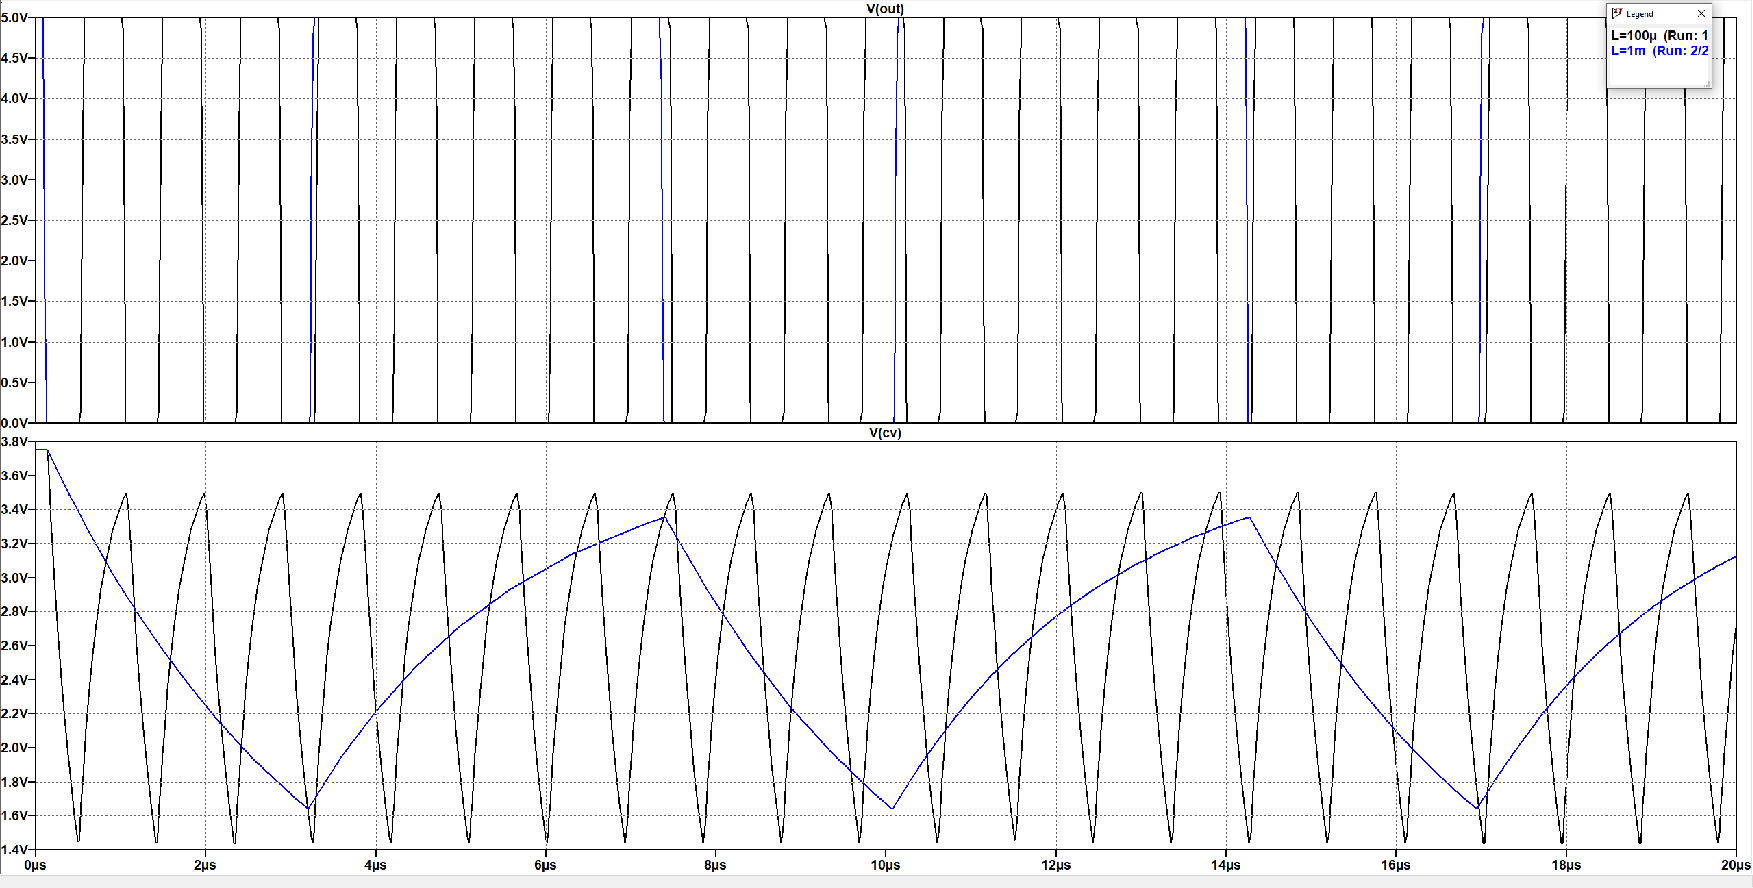
\includegraphics[width=1\linewidth]{fahrzeugerkennung/RL_Oszillator_vergleich2_ZB.pdf}
    \caption{Vergleich des NE555-Oszillators bei unterschiedlichen L}
\end{figure}

Eine Verzehnfachung der Induktivität führt zu einer Reduktion der Oszillatorfrequenz um den Faktor 10.

\begin{equation} \label{iq:f_NE555}
    f \propto \frac{1}{L}
\end{equation} 

\pagebreak
\subsubsection{Messung paramagnetischer Metalle}
Da nicht alle Metalle ferromagnetische Eigenschaften haben werden viele Stoffe wie Aluminium. Kupfer oder diverse Legierungen
von einer niederfrequenten Messung der Induktivität nicht wahrgenommen. Ein Effekt, welcher bei elektrischen Leitern abhilfe schaffen kann, sind 
die Eddy Currents. Wenn in einem Leiter ein magnetischen Feld einwirkt erzeugt dieses im Objekt Ströme, die wiederum ihr eigenes magnetische Feld erzeugen.
Die fließenden Ströme erzeugen im Objekt Ohmsche Verluste, welche normalerweise unerwünscht sind. Sie wirken auch einer Änderung der magnetischen Feldes entgegen,
da sie selbst Energie brauchen um ihre Richtung zu ändern. Je größer die Frequenz der eingespeisten Felddichte $B$ desto stärker wirkt die 
Flussdichte $B_{eddy}$ senkend auf die Gesamtflussdichte und so auf den magnetischen Fluss $\Phi$. 
Nach der Gleichung \ref{eq:L_phi} reduziert sich die Induktivität mit zunehmender Frequenz.


\begin{figure}[H]
    \centering
    \includegraphics[width=0.6\linewidth]{fahrzeugerkennung/Eddy_Currents.pdf}
    \caption{Eddy Currents in einem Leiter}
\end{figure}

Bei sehr hohen Frequenzen ist jedoch zu beachten, dass der Skin-Effekt die Querschnittsfläche, durch die der Wechselstrom fließen kann,
reduziert. Somit nimmt der Effekt der Eddy-Currents ab. Diese Phänomene werden jedoch nicht in dieser Arbeit behandelt, da sie außerhalb des Rahmens der 
Fahrzeugerkennung liegen. 

\paragraph{LC Oszillatoren}\mbox{}\\

Im Vergleich zum RL-Oszillator, der über eine astabile Kippstufe lauft, kann ein LC Oszillator seine Resonanzfrequenz nur durch das verstellen der Induktivität und der Kapazität 
eines Kondensators verändern. Zudem gibt es in der Theorie keine Wirkverluste, da die Energie abwechselnd zwischen magnetischer und elektroscher Energie umgewandelt wird. In der Realität gibt es jedoch
ohmsche Verluste, die zu einem Abklingen der Schwingung führen. Es braucht daher ein aktives Glied wie ein Transistor oder ein Operationsverstärker, der den Oszillator mit Energie versorgt.
\\
Der zeitliche Verlauf einer ungedämpften Schwingung kann in LTSPice simuliert werden indem wir eine Sprungfunktion auf ein LC Glied geben und einen Widerstand in Serie zum Kondensator oder zur
Spule geben.

\begin{figure}[H]
    \centering
    \includegraphics[width=0.6\linewidth]{fahrzeugerkennung/LC_Parallel.pdf}
    \caption{Parallelschwingkreis in LTSpice}
\end{figure}

\begin{figure}[H]
    \centering
    \includegraphics[width=1\linewidth]{fahrzeugerkennung/gedämpfte_schw.pdf}
    \caption{Gedämpfte Schwingung}
\end{figure}

Aus der Simulation ergibt sich über eine Cursormessung für die angegebenen Werte $L = \SI{100}{\milli\henry}$ und $C = \SI{100}{\milli\farad}$ eine Resonanzfrequenz einen Wert von $f = 15.85Hz$. Die Resonanzfrequenz für einfache LC-Schwingkreise lässt sich mit der
Thomsonschen Schwingungsgleichung errechnen:

\begin{equation} \label{eq:thomson}
    f = \frac{1}{2 \cdot \pi \sqrt{L \cdot C}}
\end{equation}

Wobei \\
$f$ = Resonanzfrequenz des LC-Gliedes\\
$L$ = Induktivität der Spule\\
$C$ = Kapazität des Kondensators\\

Wenn man die Werte $L = \SI{100}{\milli\henry}$ und $C = \SI{100}{\milli\farad}$ ind die Gleichung \ref{eq:thomson} einsetzt erhält man eine Resonanzfrequenz von $f = 15.915Hz$.
Allgemein tritt in LC-Glieder bei einer Phasenlage von $\varphi_{LC} = 180^{\circ}$ und bei der Frequenz nach der Thomsonschen Gleichung \ref{eq:thomson}  Resonanz auf. 

\paragraph{Einfluss von Induktivitätsänderungen auf LC-Oszillatoren}\mbox{}\\

Für die Fahrzeugerkennung ist es von Relevanz zu wissen wie die Frequenz dieser Oszillatoren auf die Änderung der Induktivität der im Boden verbauten Spule reagiert.
Wenn eine Parklücke frei ist besitzt die Spule eine Induktivität von $L_{0}$ und hat nach der Thomsonschen Gleichung \ref{eq:thomson} eine Resonanzfrequenz $f_{0}$. Für kleine Änderungen $\Delta L$ kann eine Näherung
der Frequenzänderung gemacht werden indem man in den Punkt $(f_{0}, L_{0})$ in den Graphen der Thomsonschen Gleichung aufgetragen über die Induktivität $L$ eine Tangente in diesen Punkt legt. Bei einer 
Kapazität von $C = \SI{1}{\micro\farad}$ erhält man folgenden Graphen: 

\begin{center}
    \begin{tikzpicture}
        
        \begin{axis}[
                axis x line=middle, 
                axis y line=middle, 
                xlabel={$L \text{ in } \si[]{\henry}$}, 
                ylabel={$f \text{ in } \si[]{\hertz}$}, 
                x=15cm/0.001,    
                y=0.0003cm,    
                grid =both,
                minor x tick num=1,
                subtickwidth=0pt,
                xtick={0,0.0001,...,0.001}, 
                ytick={0,5000,...,30000}, 
                xmin=0,  
                xmax=0.0011,   
                ymin=0,  
                ymax=32000,  
                scale = 0.7 
        ]
        
        \addplot [blue, thick, samples at={0,0.000001,0.000005,0.00001,...,0.0002,0.0003,0.0004,...,0.002}] {1/(2*pi*sqrt(x*1e-6))};
        \addplot[mark=none, red, thick] coordinates {(0, 20000) (0.4e-3, 0.1e4)};
        \addplot[mark=none, black, dashed] coordinates {(0, 1.4e4) (0.13e-3, 1.4e4)};
        \addplot[mark=none, black, dashed] coordinates {(0.13e-3, 0) (0.13e-3, 1.4e4)};
        \node[label={45:{($f_{0}$,$L_{0}$)}},circle,fill,inner sep=2pt] at (axis cs:0.13e-3,1.4e4) {};
        \node[label={45:{$L_{0}$}},circle,fill,inner sep=2pt] at (axis cs:0.13e-3,0) {};
        \node[label={45:{$f_{0}$}},circle,fill,inner sep=2pt] at (axis cs:0,1.4e4) {};
    \end{axis}
    \end{tikzpicture}
\end{center}

Mit dieser Näherung kann man mit des Differentials der Thomsonschen Gleichung \ref{eq:thomson} die Änderung des Funktionswertes $f(L \pm \Delta L) = \Delta f \approx df$ 
\begin{align*} \label{eq:df_L}
    df = \frac{\partial f}{\partial L}\bigg|_{L_{0}} \cdot dL \\ 
    df = \frac{\partial}{\partial L}  \left (  \frac{1}{2 \pi \sqrt{L_{0}C}} \right ) \Delta dL \\
    df = - \frac{1}{4 \pi} (L_{0}C)^{-\frac{3}{2}} \cdot \Delta L
\end{align*}

Für relative Änderungen der Induktivität $\Delta L$ um den Wert $L_{0}$ gilt:

\begin{equation} \label{eq:f_df}
    \frac{df}{f_{0}} =  -\frac{1}{2C} \cdot \frac{\Delta L}{L_{0}}
\end{equation}

Das bedeutet, dass eine kleine relative Änderung der Inuktivität $\frac{\Delta L}{L_{0}}$ bei gleicher Kapazität $C$ für eine halb so große relative Änderung in der Frequenz führt. 
Dieser Ansatz gilt nur bei kleinen $\Delta L$.

\paragraph{Messung der Frequenz eines Colpitts-Oszillator}\mbox{}\\

Der Colpitts-Oszillator ist eine Variante des LC-Oszillator und wird in der Praxis oft mit einem aktiven Element betrieben. Im Vergleich zu einem einfachen LC-Glied besitzt dieser Oszillator
zwei Kondensatoren. Das Schaltbild sieht so aus:

\begin{figure}[H]
    \centering
    \includegraphics[width=0.3\linewidth]{fahrzeugerkennung/Colpitts_LC.pdf}
    \caption{Colpitts LC-Glied}
\end{figure}

Dieses LC-Glied wird als Rückkoppelglied eingesetzt und sorgt für die nötige Phasendrehung von $\varphi_{LC} = 180^{\circ}$. Wie man in der obigen Abbildung sehen kann liegen die Kondensatoren 
$C_{1}$ und $C_{2}$ in Serie. Es ergibt sich daher eine Gesamtkapazität von $C_{ges}$.

\begin{equation} \label{eq:c_gescolpitts}
    C_{ges} = \frac{C_{1} \cdot C_{2}}{C_{1} + C_{2}}
\end{equation}
Durch einsetzen in die Thomsonsche Gleichung erhält man für die Resonanzfrequenz eines Colpitts-Oszillator:
\begin{equation} \label{eq:colpitts}
    f = \frac{1}{2 \cdot \pi \sqrt{L \cdot \left( \frac{C_{1} \cdot C_{2}}{C_{1} + C_{2}} \right) }}
\end{equation}

Wobei \\
$f$ = Resonanzfrequenz des Colpitts-Oszillator\\
$L$ = Induktivität der Spule\\
$C_{1}$ = Kapazität des Kondensators $C_{1}$\\
$C_{2}$ = Kapazität des Kondensators $C_{2}$\\

\pagebreak
Das aktive Element wird an die Anschlüsse der Spule angeschlossen muss selbst eine Phasendrehung von 180° liefern. Zusätzlich muss die Verstärkung des Gliedes größer als 1 damit eine dauerhafte 
Schwingung entstehen kann. Mit einem Operationsverstärker muss der nicht invertierende Eingang auf eine Bezugsspannung gelegt werden. Diese Bezugsspannung wird of in die Mitte des Versorgungsspannungsbereich
gelegt. Bei einem Spannungsbereich von $\SI{0}{\volt}$ bis $\SI{5}{\volt}$ ist eine Bezugsspannung von $\SI{2,5}{\volt}$ sinnvoll. Der invertierende Eingang wird an das Colpitts LC-Glied angeschlossen. Der Ausgang des Operationsverstärker wird über
einen Widerstand an das LC-Glied geschalten, damit das Rückkoppelglied besser vor übersteuerungen am Ausgang des Operationsverstärkers geschütz ist. 

\begin{figure}[H]
    \centering
    \includegraphics[width=0.4\linewidth]{fahrzeugerkennung/Colpitts_active.pdf}
    \caption{Aktiver Colpitts-Oszillator}
\end{figure}

Wenn man nun verschiedene Werte für Induktivität einsetzt ergibt sich durch die Simulation dieses Schaltbildes folgende Zeitsignale für den Ausgang des Operationsverstärker OUT und der Spannung SINE:

\begin{figure}[H]
    \centering
    \includegraphics[width=1\linewidth]{fahrzeugerkennung/Colpitts_active_ZB.pdf}
    \caption{Zeitsignale Colpitts-Oszillator}
\end{figure}

Es ist ersichtlich, dass dass eine Zunahme der Induktivität zu einer Abnahme in der Frequenz der beiden Signale führt.
\pagebreak
\subsection{RS485 Bussystem}
\subsubsection{Benutzte Standards}
\paragraph{ASCII}\mbox{}\\
ASCII ist eine amerkanischer Standard zur Kodierung einer 7 Bit langen folge. Dieser Standard ermöglicht es Zeichen wie 'A' oder 'b' sowie auch Zahlen und gewissen Sonderzeichen in Bits umzusetzen. 
\paragraph{USB}\mbox{}\\

Unter USB versteht man eine serielles Bussystem, welches dazu dient Peripherie Geräte an einen Computer zu verbinden. USB ermöglicht es Geräte während der Laufzeit des Betriebsssystems anzustecken und wieder zu entfernen.
Je nach Version des USB Standards ist es möglich unterschiedliche Datenraten und Leistungen zu verwenden, wobei neuere Standards Rückkompatibel zu alten Versionen sind. Für die Ansteeurng des Bussystems ist es notwendig einen Comupter anzuschließen. 
Der USB Standard bietet sich hier an, da er weit verbreitet ist und daher mit vielen Computern kompatibel ist.


\paragraph{UART}\mbox{}\\

Unter UART versteht man eine eine asynchrone serielle Schnittstelle. Die elektrische Schnittstelle braucht daher auch keine Taktleitung die dem Empfänger der Daten mitteilt wann er zu lesen hat. Stattdessen gibt es zwei Datenleitungen nämlich eine 
für das Senden TX und eine für das Lesen RX. Auf diesen Datenleitungen befinden sich nur die Bitströme des Empfängers und des Senders. Sie besitzen einen Ruhepegel von logisch 1.
UART synchronisiert sich idem es beim Start der Daten ein Startbit schickt, welche Sender und Empfänger synchronisiert. 
Diese beiden Geräte brauchen daher auch genaue interne Uhren um sich über den Zeitraum des Datenaustausches synchron zu halten.
Die Dauer diese Datenaustausches hängt vor allem von der Bitrate auch genannt Baudrate ab aber auch die Konfiguration der Anzahl von Datenbits und Paritätsbits haben Einfluss auf diese Größe. 
\\
In der folgenden Abbildung ist zeitliche Verlauf einer Datenleitung dargestellt es wird das Zeichen 'A' in ASCII codiert übertragen bei einer Baudrate von 57600 Zeichen pro Sekunde.

\begin{figure}[H]
    \centering
    \includegraphics[width=1\linewidth]{fahrzeugerkennung/UART_example.pdf}
    \caption{Beispiel einer UART Zeichenübertragung}
\end{figure}

\paragraph{RS485}\mbox{}\\

RS485 ist ein Standard für eine physikalische Schnittstelle für Datenübertragung von UART Daten. Er besitzt zwei symmetrische Leitung oft mit A und B bezeichnet, dessen Differenzspannung für die Auswertung
des Datenstromes herangezogen wird. Er ist dafür ausgelegt mehrere Geräte an die gleiche Leitungen anzuschließen. Die maximale Anzahl an Geräten ist mit 32 fix vorgegeben. Es ist zusätzlich notwendig die Spannungen 
$U_{A}$ und $U_{B}$ im Ruhezustand über einen IC oder einen Spannungsteiler auf fixe Potentiale zu legen. Der Spannungsteiler muss wie folgt aussehen um dem Standard zu entsprechen.

\begin{figure}[H]
    \centering
    \includegraphics[width=0.15\linewidth]{fahrzeugerkennung/RS485_bias.pdf}
    \caption{RS485 Widerstandsnetzwerk}
    \label{fig:rs485_bias}
\end{figure}

Um diese physikalische Umwandlung zu ermöglichen ist eine Umwandlungs IC erforderlich. In dieser Arbeit wurde ausschließlich der MAX485CSA für Wandlung zwischen den Standardpegeln der UART
und die der RS485 Schnittstelle verwendet.

Dieser IC ist Bussfähig und kann daher seine Ausgänge hochohmig machen. Er besitzt folgende Eingänge und Ausgänge:
\begin{itemize}
    \item \textbf{!RE: Read enable} \\
    Wenn dieser Eingang auf logisch 0 gesetzt ist wertet der IC des Differenzsignal $U_{AB}$ aus und liefert des Ergebnis an den Ausgang RO.
    Ansonsten setzt er den Ausgang RO in den Tristate beziehungsweise auf hochohmig.
    \item \textbf{DE: Data enable} \\
    Wenn dieser Eingang auf logisch 1 gesetzt ist wird die Spannung am Eingang DI in die zugehörigen Pegel $U_{A}$ und $U_{B}$ umgewandelt.
    Ansonsten setzt er den Eingang DI in den Tristate beziehungsweise auf hochohmig.
    \item \textbf{RO: Read out} \\
    Ist die eingelesene Spannung die sich logisch aus der Differenzspannung $U_{AB}$ ergibt wenn !RE auf logisch 0 ist.
    \item \textbf{DI: Data In} \\
    Ist die eingehende Spannung die auf die RS485 Schnittstelle geschrieben werden soll, wenn der Eingang DE auf logisch 1 ist.
\end{itemize}

Die Auswertung der Differenzspannung $U_{AB}$ kann auch in der folgenden Tabelle aus dem Datenblatt des MAX485CSA entnommen werden. 

\begin{figure}[H]
    \centering
    \includegraphics[width=0.6\linewidth]{fahrzeugerkennung/RS485_receiving_table.pdf}
    \caption{Logische Tabelle für $U_{AB}$}
\end{figure}

In der folgenden Abbildung wird wieder an 'A' ASCII kodiert versendet nur dieses mal wird eine RS485 Schnittstelle mit den entsprechenden Pegeln verwendet verwendet.
In blau ist die Spannung $U_{A}$ und in orange die Spannung $U_{B}$ zu sehen. Darunter befindet sich das logische UART Signal am Ausgang RO. 

\begin{figure}[H]
    \centering
    \includegraphics[width=1\linewidth]{fahrzeugerkennung/RS485_example.pdf}
    \caption{Beispiel einer RS485 Zeichenübertragung}
\end{figure}

\paragraph{RJ45}\mbox{}\\
Um die Anzahl der Kabel zu minimieren und um das Anschließen von Geräten an den Bus einfach zu halten ist ein
mehradriger Stecker mit zugehörigem Kabel nötig.\\
Der RJ-45 Stecker ist eine genormter Stecker und besitzt insgesamt 8 Adern und ist für Kommunikationsanschlüsse gedacht. Er kann daher größere Datenraten zulassen und viele auf dem
Markt vorhandene Kabel haben zusätzliche Abschirmungen, die die Datenleitungen vor elektrischen Störungen schützen. 

\begin{figure}[H]
    \centering
    \includegraphics[width=0.6\linewidth]{fahrzeugerkennung/RJ45_connectors.pdf}
    \caption{RJ45 Steckerbuchse und Kabel}
\end{figure}



\subsubsection{Aufbau}

Das Bussystem wir über eine Master Slave Struktur verwaltet was heißt das nur das ein einzelnes Master-Gerät als erstes andere Teilnehmer am Bus ansprechen kann.
Slave-Geräte können nur nach Anfrage des Masters auf den Bus schreiben. Neben der Steuerung der Kommunikation sollte das Master-Gerät aus praktischen Gründen ebenfalls die Slave-Geräte
mit Energie versorgen und ihnen eindeutige Adressen zuweisen können. \\

In den unteren Abbildungen sind der logische Aufbau und der physikalische Aufbau zu sehen.
Auf die einzelnen Funktionen diverser Leitungen wird in den folgenden Paragraphen eingegangen.

\begin{figure}[H]
    \centering
    \includegraphics[width=1\linewidth]{fahrzeugerkennung/übersicht_bus.pdf}
    \caption{Logische Übersicht des Bussystems}
\end{figure}

\begin{figure}[H]
    \centering
    \includegraphics[width=1\linewidth]{fahrzeugerkennung/übersicht_irl.pdf}
    \caption{Physische Übersicht des Bussystems}
\end{figure}
Ganze rechts oben in schwarz ist der RaspberryPi der hier als Computer dient es kann aber auch ein anderer Computer verwendet werden. Unterhalb des RaspberryPi ist der USB-RS485 Wandler der mit einem USB-Kabel
am RaspberryPi angeschlossen ist und von an einer Versorgungsspannung hängt. Der USB-Rs485 Wandler ist wiederrum mit einem RJ45-Kabel an einen Slave verbunden. In diesem Bild sind zwei Slaves an das Bussystem geschlossen worden.
Es können aber bis zu 31 sein. Ganz rechts ist der Leitungsabschluss der in Abbildung \ref{fig:rs485_bias} zu sehen ist.
\\ \\
Die elektrische Belegung der Leitungen ist wie in der folgenden Tabelle festgelegt worden. Mit dieser Belegung ist es möglich die Slave-Geräte an den RS485 Datenbus zu legen,
sie mit Spannung zu versorgen und die Adressvergabe mit einer zusätzlichen Logikleitung zu regeln. 

\begin{table}[h]
    \centering
    \begin{tabular}{|c|c|c|c|}
        \hline
        \textbf{Pinnummer} & \textbf{Farbe} & \textbf{Netz} & \textbf{Beschreibung}                      \\ \hline
        1                  & Orange / weiß  & GND           & Masse                                      \\ \hline
        2                  & Orange         & +5V           & 5 Volt Versorgungsspannung                 \\ \hline
        3                  & Grün / weiß    &               & unbelegt                                   \\ \hline
        4                  & Blau           & A             & RS485 positives Datensignal                \\ \hline
        5                  & Blau / weiß    & B             & RS485 negatives Datensignal                \\ \hline
        6                  & Grün           & VCC           & Positive Versorgungsspannung +9V bis 30V   \\ \hline
        7                  & Braun / weiß   & GND           & Masse                                      \\ \hline
        8                  & Braun          & ADR           & Logiksignal zur Vergabe der Slave Adressen \\ \hline
    \end{tabular}
    \caption{RJ45 allgemeine Pinbelegung}
\end{table}

\paragraph{Funktion der Adresslogikleitung}\mbox{}\\

Da alle Teilnehmer des RS485-Busses parallel an den Datenleitung A und B liegen kann der Master sie voneinander nicht unterscheiden. Dieses Probleme beseitigt die Adressleitung, welche
die einzelnen Geräte logisch aneinanderreiht.

\begin{figure}[H]
    \centering
    \includegraphics[width=1\linewidth]{fahrzeugerkennung/adress_function.pdf}
    \caption{Anordnung der Slave-Geräte mit Adresslogikleitung}
\end{figure}

Jedes Slave-Gerät setzt seine Adresslogikleitung über einen Pullup-Widerstand auf logisch 1 wenn es keine Adresse zugeordnet bekommen hat.
Als erstes in der Reihe ist der Master, der seine Adresslogikleitung auf logisch 0 setzt und so dem ersten Gerät in der Kette bekannt gibt, dass es eine Adresse zugewiesen bekommt. Wenn es
diese Adresse bekommen hat legt das Slave-Gerät seine ausgehende Adresslogikleitung ADRO auf logisch 0. So kann das nächste Gerät in der Kette erkennen, dass es eine Adresse zugewiesen kriegt, 
indem es auf die eingehende Adressleitung ADRI achtet.\\
In den folgenden Abbildungwn sieht man wie die Geräte über den RJ45 Stecker elektrisch am Bus hängen. Der Master hat nur einen Stecker und hat seine Adresslogikleitung fix auf logisch 0 gelegt.
Die Slaves hingegen brauchen zwei Stecker um die Adresskette zu bilden und unterscheiden zwischen eingehender Adresslogikleitung ADRI und ausgehender Adresslogikleitung ADRO. \\
Wenn jedoch die Slaves falsche herum angeschlossen werden und ADRI und ADRO vertauscht sind kann dieser Fehler vom Mikrokontroller erkannt und behoben werden. Die genauen Details dieser Funktion 
werden in späteren Abschnitten erklärt. 

\begin{figure}[H]
    \centering
    \includegraphics[width=0.6\linewidth]{fahrzeugerkennung/RJ45_slave.pdf}
    \caption{RJ45 Pinbelegung des Slave-Geräts}
\end{figure}

\begin{figure}[H]
    \centering
    \includegraphics[width=0.3\linewidth]{fahrzeugerkennung/RJ45_master.pdf}
    \caption{RJ45 Pinbelegung des Master-USB-Geräts}
\end{figure}

\paragraph{Versorgungsleitungen VCC und GND}\mbox{}\\

Da es für jeden Parkplatz ein Slave-Gerät gibt ist die Länge der Busleitung nicht unbeträchtlich. Es kann so entlang der Leitung zu abfällen in der Versorgungsspannung aufgrund des Widerstands der langen Leitung.
Um dem entgegenzuwirken muss die Versorgungsspannung VCC bezogen auf Masse größer als die benötigte Spannung an den Geräten sein. Die Slave-Geräte besitzen alle einen Linearregler der für einen konstante Spannung von 5V sorgt.
Die Eingangsspannung des Spannungsreglers muss je nach Ausführung um eine gewisse Differenzspannung größer sein als die am Ausgang benötigte Spannung sein. Dieser Wert wird als \textit{Dropout Voltage} bezeichnet. 
Für den IC L78L05ACD lässt sich aus dem Datenblatt folgende Spannung nachlesen: $\SI{2}{\volt}$

\begin{figure}[H]
    \centering
    \includegraphics[width=1\linewidth]{fahrzeugerkennung/L78L05_characteristics.pdf}
    \caption{Elektrische Eigenschaften des L78L05ACD}
\end{figure}

Daraus lasst sich schließen dass der IC mindestens eine Spannung von $\SI{7}{\volt}$ braucht um zu funktionieren. Als Eingangsspannung für alle Messung wurde $\SI{9}{\volt}$ verwendet. Nach Datenblatt ist die Eingangsspannung auf 
einen Maximalwert von $\SI{30}{\volt}$ beschränkt. Es ist zu beachten, dass eine Erhöhung der Eingangsspannung zu mehr Verlusten am Linearregler führt und somit für eine schlechte Effizienz sorgt.

\subsubsection{Implementation eines eigenen Protokolls}

RS485 spezifiziert keine Protokoll unter welchem Busteilnehmer untereinander kommunizieren. Es gibt bereits viele fertige Lösung wie zum Beispiel Modbus, welches auf einer Master/Slave-Architektur basiert. Es ist aber auch möglich ein eigenes Protokoll zu erstellen.
In den folgenden Absätzen wird der Aufbau und die Funktion eines eigen implementierten Protokoll, für die Fahrzeugerkennung, erklärt.
\pagebreak
\paragraph{Aufbau von Datenframes}\mbox{}\\

Mit UART ist es möglich, unter der Konfiguration von 8 Datenbits, eine Byte pro Datenaustausch zu senden. Diese Bytes bilden die Grundbausteine unseres sogenannten Datenframes, welcher eine Aneinanderreihung von Bytes ist. Jedes Byte
kann eine unterschiedliche Funktion haben. Es kann zu einem einfache Daten beinhalten oder dem anderen Teilnehmer bestimmte Steueranfragen mitteilen. Die Datenframes sind in folgende Grundstruktur aufgeteilt.

\begin{table}[h]
    \centering
    \begin{tabular}{|c|c|c|c|c|c|c|c|c|c|c|c|c|c|c|c|c|}
    \hline
    \multicolumn{17}{|c|}{\textbf{Datenframe}}                                                                                                             \\ \hline
    \textbf{Byte}     & 0     & 1           & 2          & 3    & 4           & 5          & 6  & 7  & 8  & 9  & 10  & 11  & 12  & 13 & 14   & 15   \\ \hline
    \textbf{Name}            & START & \multicolumn{2}{c|}{ADR} & CTRL & \multicolumn{2}{c|}{ARG} & \multicolumn{8}{c|}{DATA\_0 bis DATA\_7} & STOP & LF   \\ \hline
    \textbf{Hexwert}    	 & 0x02  &             &            &      &             &            & \multicolumn{8}{c|}{}                    & 0x03 & 0x11 \\ \hline
    \end{tabular}
    \caption{allgemeiner Aufbau eines Datenframes}
\end{table}

\begin{itemize}
    \item \textbf{START, STOP und LF} \\
    Diese Bytes helfen den Geräte den Anfang und des Ende eines Frames zu erkennen. Das START-Byte signalisiert den Anfang des Datenframes und hat einen fixen von \texttt{0x02} während das Byte STOP mit dem 
    fixen Hexwert von \texttt{0x03} das Ende das Ende signalisiert. Zusätzlich kommt am Ende noch das LF-Byte mit einem Hexwert von \texttt{0x11}. In ASCII kodiert ist das das Zeichen einer neue Zeile in einem Text und ist vorallem nützlich, da
    viele Bibliotheken dieses Zeichen als Endzeichen zu Datenauslesung aus einem seriellen Buffer verwenden.
    \item \textbf{ADR} \\
    Jedes Gerät am Bus ist unter seiner eigenen Adresse erreichbar welche aus zwei Bytes besteht. Die Adressen werden über den Master verteilt, der eine fixe Adresse von \texttt{0x01} besitzt. 
    Zusätzlich sind alle Slaves unter einer Broadcastadresse von \texttt{0x00} erreichbar. Es ergibt sich mit zwei Bytes eine Adressraum der Größe $2^{16} = 65536$ inklusive Master und Broadcast.
    \item \textbf{CTRL} \\
    Das Kontrollbyte CTRL signalisiert einen bestimmten Steuerbefehl. Mit ihm kann man eine Frequenzmessung der Spule an einem Slave auslösen oder einezelne LEDs ein- und ausschalten.
    
    \item \textbf{ARG} \\
    Die Argumentbytes ARG1 und ARG2 geben dem Steuerbefehl zusätzliche Daten mit. 
    So kann man zum Beispiel zwischen LED1 und LED0 und einschalten und ausschalten unterscheiden. 
    
    \item \textbf{DATA} \\
    Hier versteht man 8 Datenbytes, die für den Austausch von größeren Werten, wie einer Frequenz von nutzen sind. Diese Datenbytes sind in ASCII kodiert um Konflikte mit den START, STOP und LF Bytes zu vermeiden. Jedes Datenbyte kann daher einen Hexwert von \texttt{0x0} bis 
    \texttt{0xF}. Der größtmögliche Wert, der sich verschicken lässt ist daher \texttt{0xFFFFFFFF} was in Dezimal einem Wert von $2^{32} - 1 = 4 294 967 294$ entspricht.
\end{itemize}

\paragraph{Steuerabläufe}\mbox{}\\

Um eine Aktion auszuführen schreibt der Master auf den Bus ein Datenframe und wartet auf die Antwort des angesprochenen Slaves. 

\begin{figure}[H]
    \centering
    \includegraphics[width=0.4\linewidth]{fahrzeugerkennung/master_slave_dataframes.pdf}
    \caption{Ablauf von Steueranfragen}
\end{figure}

Die Art des Steuerbefehls wird durch das CTRL-Byte angegeben un definiert so die Inhalte der Bytes. Es muss aber zwischen einen Master Datenframe und einem Slave-Response Datenframe unterschieden werden. 
In den nächsten Abbildung werden die möglichen Steuerbefehle für Master und Slave in Tabellenform angeführt.

\begin{sidewaysfigure}
    \centering
    \includegraphics[width=1\linewidth]{fahrzeugerkennung/master_datenframe.pdf}
    \caption{Master Datenframe}
\end{sidewaysfigure}

\begin{sidewaysfigure}
    \centering
    \includegraphics[width=1\linewidth]{fahrzeugerkennung/slave_response_datenframe.pdf}
    \caption{Slave Response Datenframe}
\end{sidewaysfigure}
\pagebreak
Um den Ablauf einer deutlicher darzustellen wird der Steuerbefehl IO1 mit Datenframe Antwort des Slaves gemessen. 
Wir erhalten folgendes Bild am Oszilloskop.

\begin{figure}[H]
    \centering
    \includegraphics[width=1\linewidth]{fahrzeugerkennung/slave_resp_measured_dataframe.pdf}
    \caption{gemessene Slave Response bei Steuerbefehl IO1}
\end{figure}

\begin{table}[h]
    \centering
    \begin{tabular}{|c|c|c|c|c|c|c|c|c|l|l|l|l|l|l|c|c|}
        \hline
        \multicolumn{17}{|c|}{\textbf{Datenframe}}                                                                                           \\ \hline
        \textbf{Byte}  & 0     & 1           & 2          & 3    & 4           & 5          & 6    & \multicolumn{7}{c|}{7-13} & 14   & 15   \\ \hline
        \textbf{Name}  & START & \multicolumn{2}{c|}{ADR} & CTRL & \multicolumn{2}{c|}{ARG} & \multicolumn{8}{c|}{DATA}        & STOP & LF   \\ \hline
        \textbf{Hex}   & 0x02  & 0x30        & 0x31       & 0x31 & 0x49        & 0x00       & 0x30 & \multicolumn{7}{c|}{0x00} & 0x03 & 0x11 \\ \hline
        \textbf{ASCII} & STX   & 0           & 1          & 1    & I           & NUL        & 0    & \multicolumn{7}{c|}{NUL}  & ETX  & LF   \\ \hline
    \end{tabular}
    \caption{ausgelesene Bytes aus einem gemessenen Datenframe}
\end{table}

Wir sehen dass die Bytes START, ETX und LF die dix zugewiesenen Werte \texttt{0x02, 0x03} und \texttt{0x11} haben. Die ADR Bytes haben ASCII dekodiert die Zeichen '0' und '1' welche zusammengezählt die Adresse 1 ergeben. 
Dies ist die fixe Adresse des Masters und stimmt auch mit unserem Master/Slave System überein, wo die Slaves Datenframes nur an den Master zurück schicken. Das Kontrollbyte CTRL hat den Hexadezimalwert \texttt{0x31} 
und entspricht ASCII dekodiert dem Zeichen '1'. Sieht man nun in der Tabelle mit den Slave-Response Datenframes nach erhalten wir den Befehl IO1. Mit diesem Befehl wird ein digitaler Ein- und Ausgang des Mikrokontroller gesteuert.
Das erste Argumentbyte ergibt ASCII dekodiert das Zeichen 'I' was laut gleicher Tabelle SET bedeutet. Das zweite Argumentbyte hat den Hexadezimalwert \texttt{0x30} welches dekodiert das ASCII Zeichen '0' ist. Dieses Zeichen gibt an,
dass der Ausgang IO0 auf logisch 0 zu schalten ist. Die Datenbytes für die den Befehl IO1 sind bis auf das erste alle von sich aus leer. Das erste Datenbyte soll bestätigen dass der Ausgang auf logisch 0 geschalten worden ist und tatsächlich steht 
diesem Byte das Zeichen '0'.  
\\ \\
Der interne C-Code des Slave generiert für den IO1 Befehl dia Antwort auf folgende weise.
\begin{listing}[H]
    \begin{minted}{c}
    unsigned char response[8] = {0, 0, 0, 0, 0, 0, 0, 0};
    IO1_OUT;
    if(argument_2 == OFF)
    {
        IO1_OFF; 
        response[0] = 0x30;
    }
    else if(argument_2 == ON)
    {
        IO1_ON;
        response[0] = 0x30;
    }
    rs485_write_frame(MASTER_MSB, MASTER_LSB, IO1, SET, NONE, response);
    \end{minted}
    \caption{Response C-Code des Slave für IO1}
  \end{listing}
\pagebreak

Das Slave-Gerät setzt IO1 als Ausgang und überprüft das zweite Argumentbyte auf dessen Inhalt und setzt den Ausgang je nachdem auf logisch 1 oder 0.

\subsection{Mikrokontroller Slave-Geräte}
\subsubsection{Überblick}
\subsubsection{Atmega328PB}
\subsubsection{Peripherie des Mikrokontrollers}
\paragraph{Spannungswandler}
\paragraph{RS485 Pegelwandler}
\paragraph{Digitale Ein- und Ausgänge}
\subsubsection{Layout des Slave-Gerätes}
\subsubsection{Gehäuse}


\subsection{USB-Master}
\subsubsection{USB-Bussadapter Gerät}
\paragraph{Überblick}
\paragraph{FT232RL}
\paragraph{Spannungsversorgung}
\paragraph{USB-C Anschluss}
\paragraph{Layout des Master-Geräts}
\paragraph{Gehäuse}

\subsubsection{Master Programm}
\paragraph{Benötigte Software}
\paragraph{Adressvergabe}
\paragraph{Frequenzauslesung}

\paragraph{Auswertung}
\paragraph{API-Post}

\subsubsection{RaspberryPi als Mastergerät}
\paragraph{SSH Remote Zugriff}
\paragraph{Code Deployment}
\paragraph{Unittest}

\pagebreak



\pagebreak


\section{Webinterface}
\def \sectionauthors {Philipp Kraft}

\subsection{Einleitung}
Das Webinterface hat auf der einen Seite die Aufgabe die Kommunikation mit der
Kennzeichenerkennung und der Fahrzeugerkennung sicherzustellen und auf der
anderen Seite die Verwaltung und Darstellung der gewonnen Daten.

\subsection{Verwendete Technologien}
\subsubsection{HTML}
\acs*{HTML} steht hierbei für \acl*{HTML} und ist eine Auszeichnungssprache
welche vom \ac*{W3C}\footnote{\url{https://www.w3.org} } entwickelt wird.
\ac*{HTML} ist De-Facto-Standard um Inhalte in Browsern darzustellen.
\acs*{HTML} ist dabei aber nicht für die visuelle Darstellung verantwortlich
sondern nur für die semantische Struktur. Der Sinn dahinter ist, dass der Inhalt
und die Vorgaben an die Darstellung möglichst gut getrennt ist. Für die
Formatierung kommt die Stylesheet-Sprache \ac*{CSS} zum Einsatz, welche
ebenfalls vom \acl*{W3C} entwickelt wird. Die aktuellste Version der \acs*{HTML}
Spezifikation ist
HTML5\footnote{\url{https://www.w3.org/2014/10/html5-rec.html.en}} und wurde am
28. Oktober 2014 vom \acs*{W3C} vorgelegt.

\begin{figure}[H]
  \centering
  \includegraphics[width=0.2\linewidth]{webinterface/html5_logo.png}
  \caption{HTML5 Logo}
\end{figure}

\paragraph{Beispielhafte HTML Seite}\mbox{}\\
Eine \acs*{HTML} Seite setzt sich aus einer Vielzahl von sogenannten Elementen
zusammen. Ein Element besteht aus einem Start Tag und aus einem End Tag, der
Inhalt wird zwischen diese Tags geschrieben. Nun folgt eine einfache HTML Seite,
welche die Grundlegenden Funktionen von HTML und CSS darlegen soll.

\begin{listing}[H]
  \begin{minted}{html}
    <!DOCTYPE html>
    <html>
    <head>
    <title>Titel</title>ü
    </head>
    <body>

    <h1>Überschrift</h1>
    <p>Paragraph</p>

    </body>
    </html>
  \end{minted}
  \caption{index.html}
  \label{lst:simple_html_site}
\end{listing}

Das Element \verb|<!DOCTYPE html>| deklariert, dass die folgende Seite den HTML5
Standard verwendet. Danach folgt mit \verb|<html>| das Wurzelelement, dass alle
anderen Elemente beinhaltet. Das \verb|<head>| Element beinhaltet verschiedene
Metadaten d.h. Daten die nicht angezeigt werden. Im oben gezeigten Beispiel
Code~\ref{lst:simple_html_site} wird nur der Title des Dokuments gesetzt, dieser
wird im Browser Tab angezeigt. Es können aber auch noch andere Daten gesetzt
bzw. eingebunden werden:

\begin{itemize}
  \item Character Set
  \item Styles
  \item Scripts
  \item Viewport
  \item Sonstige Metainformationen (Author, Keywords)
\end{itemize}

\begin{figure}[H]
  \centering
  \frame{\includegraphics[width=1\linewidth]{webinterface/simple_html_site.png}}
  \caption{Einfache HTML Seite von \citeurl[]{html5logo}}
\end{figure}

\subsubsection{CSS}
Wie bereits angesprochen ist \ac*{CSS} für die Formatierung bzw. die visuelle
Darstellung der einzelnen HTML-Elemente verantwortlich. Der Standard wird wie
bei HTML vom \acs*{W3C} spezifiziert und die aktuellste Version ist CSS3 was so
viel bedeutet wie \acs*{CSS} Level 3, wobei nur einzelne Teile als Empfehlung
durch das \acs*{W3C} vorgelegt wurden, beispielweise das CSS Color Module Level
3\footnote{\url{https://www.w3.org/TR/css-color-3}}. Um die Funktion
darzustellen wird die vorherige HTML Seite nun mit CSS ergänzt.

\begin{listing}[H]
  \begin{minted}{css}
    body {
      background-color: deepskyblue;
    }

    h1 {
      color: white;
      text-align: center;
      font-family: verdana;
    }

    p {
      color: wheat;
      font-family: verdana;
      font-size: 20px;
    }
  \end{minted}
  \caption{style.css}
\end{listing}

Nun muss dieses Stylesheet nur noch im \verb|<head>| Tag mit\\
\mintinline{css}{  <link rel="stylesheet" href="style.css">} eingebunden werden.

\begin{figure}[H]
  \centering
  \frame{\includegraphics[width=1\linewidth]{webinterface/simple_html_site_with_css.png}}
  \caption{Einfache HTML Seite mit CSS}
\end{figure}

Es lässt sich nun erkennen, dass sich die Webseite deutlich verändert hat. Dabei
bieten HTML und CSS bieten noch viel mehr Funktionen, eine ausführliche
Dokumentation der Funktionen sind auf der Website
w3schools\footnote{\url{https://www.w3schools.com/html} und
\url{https://www.w3schools.com/css}} zu finden.

\subsubsection{JavaScript}
Es folgt nun eine weitere sehr wichtige Technologie und die meist verwendete
Programmiersprache überhaupt laut der Stack Overflow Developer Survey
2020\footnote{\url{https://insights.stackoverflow.com/survey/2020}}. \ac*{JS}
ermöglicht es dynamische Webseiten zu erstellen, dabei wird der Code direkt
lokal im Browser ausgeführt. Jedoch ist JavaScript nicht mehr nur auf das
Frontend\footnote{Grafische Benutzeroberfläche mit der der Benutzer interagiert}
mehr beschränkt, es möglich mit Frameworks wie Node.js auch
Backend\footnote{Verarbeitung von Daten auf beispielsweise einem Server}
Applikationen zu schreiben und somit ist es möglich Full-Stack\footnote{Front-
und Backend}-Anwendungen vollständig mit \acl*{JS} zu entwickeln. Eine der
wichtigsten Anwendungsgebiete ist die Manipulation von Elementen über das
\ac*{DOM}. Der Standards wird unter dem Namen ECMA Script von der Organisation
Ecma International\footnote{\url{https://www.ecma-international.org}}
veröffentlicht und die aktuellste Version ist \textbf{ECMA-262}.

\subsubsection{PHP}
\ac*{PHP} ist eine Skriptsprache um dynamische Webseiten zu realisieren, jedoch
wird nicht wie bei \acl*{JS} der Code auf dem Client ausgeführt sondern auf dem
Server, dort wird die HTML-Ausgabe generiert und dem Client zugesendet. Somit
ist es nicht möglich den Code als Benutzer zu betrachten. Grundsätzlich ist PHP
als synchrone Sprache geplant worden, es ist jedoch auch möglich asynchron zu
Programmieren um die Performance zu steigern. Die aktuellste Version ist
\acs*{PHP} 8\footnote{\url{https://www.php.net/docs.php}}.


\subsubsection{TailwindCSS}
Es gibt eine Vielzahl von CSS-Frameworks, das Ziel ist ein einfacheres und
schnelleres erstellen von Webseiten, dazu gehören neben TailwindCSS folgende
relevanten Frameworks.

\begin{itemize}
  \item Bootstrap (\url{https://getbootstrap.com})
  \item Foundation (\url{https://get.foundation})
  \item Materialize (\url{https://materializecss.com})
\end{itemize}

Viele von diesen CSS Frameworks verwenden vorgefertigte Components welche direkt
verwendet werden können, dies führt dazu, dass die Entwicklung sehr rasch ist.
Dort unterscheidet sich TailwindCSS von den anderen CSS Frameworks, dort
existieren sogenannte Utility-Classes, diese können direkt im \acs*{HTML} auf
die einzelnen Elemente angewendet werden.

%\subsubsection{Vue}

\subsubsection{Laravel}
Laravel\footnote{\url{https://laravel.com/}} ist ein Open-Source PHP-Framework,
es erleichtert die Entwicklung und erhöht die Sicherheit und auch durch die
zahlreichen First-Party-Packages bietet Laravel ein sehr hochwertiges Ecosystem.
Da Laravel ein sehr wichtiger Bestandteil des Webinterfaces ist wird später noch
genauer auf die einzelne Funktionen des Frameworks eingegangen. Laravel wird
seit Juni 2011 entwickelt und erhält jährlich eine neue Version, aktuell ist
Laravel 8 die neuste Version.\\

Das Framework folgt dem sogenannten \ac*{MVC} Muster das bedeutet, dass die
Programmierlogik in drei verschiedene Teile unterteilt wird. Der Sinn dahinter
ist, dass die Anwendung dadurch sehr flexibel ist und später leichter erweitert
werden kann oder einzelne Teile wiederverwendet werden können.

\begin{itemize}
  \item \textbf{Model} \\
  Hier befindet sich die Datenstruktur der Anwendung. In Laravel kann dies
  beispielsweise das Model \verb|User| sein.
  \item \textbf{View} \\
  In der View befindet sich die Präsentationsebene, im Fall von Laravel sind das
  Components und Layouts.
  \item \textbf{Controller} \\
  In den Controllern der Anwendung befindet sich die Logik um beispielsweise
  durch das Absenden eines Formulares einen Eintrag in der Datenbank zu
  erstellen. 
\end{itemize}

Ein Anfrage auf eine Webseite läuft in 6. Schritten ab:

\begin{itemize}
  \item \textbf{1. Schritt:} Der Benutzer führt eine HTTP-Anfragemethode aus
  \item \textbf{2. Schritt:} Die Anfrage wird geroutet
  \item \textbf{3. Schritt:} Der Controller interagiert mit dem Model
  \item \textbf{4. Schritt:} Das Model greift auf die Datenbank zu
  \item \textbf{5. Schritt:} Der Controller liefert die Daten an eine View
  \item \textbf{6. Schritt:} View mit den Daten werden an den Client gesendet
\end{itemize}

\begin{figure}[H]
  \centering
  \includegraphics[width=1\linewidth]{webinterface/mvc_laravel.pdf}
  \caption{Laravel MVC Muster}
\end{figure}

\paragraph{Routing}\mbox{}\\
In Laravel erfolgt durch ein Routefile unter \verb|routes/web.php|. API Requests
haben ein eigenes Routefile unter \verb|routes/api.php| und erhalten einen
\verb|/api| Prefix. Diese Dateien werden dann automatisch durch einen Service
Provider von Laravel geladen.\\

Der Laravel Router erlaubt folgende HTTP-Anfragemethoden:
\begin{itemize}
  \item \textbf{GET} (Fordert Ressource an)\\
  \mintinline{php}{  Route::get($uri, $callback);}
  \item \textbf{POST} (Neue Ressource erstellen)\\
  \mintinline{php}{  Route::post($uri, $callback););}
  \item \textbf{PUT} (Ressource ersetzen oder erstellen)\\
  \mintinline{php}{  Route::put($uri, $callback);}
  \item \textbf{PATCH} (Ressource ändern)\\
  \mintinline{php}{  Route::patch($uri, $callback);}
  \item \textbf{DELETE} (Löscht Ressource)\\
  \mintinline{php}{  Route::delete($uri, $callback);}
  \item \textbf{OPTIONS} (Liste von unterstützen Methoden des Servers)\\
  \mintinline{php}{  Route::options($uri, $callback);}
\end{itemize}

Im folgenden Ausschnitt Code~\ref{lst:user_routes} werden ein Teil der Routen
von den Benutzern dargelegt. Dabei lässt sich erkennen, dass die Routen sich in
einer Gruppe befinden, welche den Prefix \verb|/admin| und die Middleware
\verb|verified| hat das bedeutet, dass der Benutzer eingeloggt sein muss um
diese Routen aufzurufen. Dabei verweisen die Routen auf einzelne Methoden im
UserController. Schlussendlich werden mit der name-Methode die Routen benannt,
damit sie später im Code einfach referenziert werden können.

\begin{listing}[H]
  \begin{minted}{php}
    <?php
    Route::group(['middleware' => 'verified', 'prefix' => 'admin'], 
    function () {
      Route::get('users', [UserController::class, 'index'])->name('users.index');
      Route::get('users/create', [UserController::class, 'create'])->name('users.create');
      Route::post('users', [UserController::class, 'store'])->name('users.store');
    });
  \end{minted}
  \caption{web.php}
  \label{lst:user_routes}
\end{listing}

\paragraph{Blade Templates}\mbox{}\\
Blade ist eine Template Engine, die mit Laravel mitgeliefert wird. Blade
erleichtert und vereinfacht das Verwenden von PHP Code in HTML, dabei wird der
Blade Syntax in normalen PHP Code compiliert. Blade Dateien werden mit der
Extension \verb|.blade.php| erstellt. Damit der Inhalt der einzelnen Seiten
dynamisch ist müssen Daten übergeben werden, dies erfolgt über die Controller.\\

Um nun Inhalt innerhalb eines Blade Files anzuzeigen verwendet Blade doppelt
Geschweifte Klammern.

\begin{listing}[H]
  \begin{minted}{php}
    Hallo, {{ $user->full_name }}.
  \end{minted}
  \caption{example.blade.php}
  \label{lst:blade_example}
\end{listing}

Im Code~\ref{lst:blade_example} wird nun auf das übergebene Model \verb|User|
zugegriffen und der Name ausgegeben.

\paragraph{Controllers}\mbox{}\\
Es besteht theoretisch die Möglichkeit die komplette Logik für die bearbeitung
von Anfragen direkt in den Route Files zu platzieren, dies ist jedoch sehr
unübersichtlich und deshalb ist es sinnvoll diese Logik in Controller Klassen
auszulagern. Dabei werden ähnliche Anfragen zusammengeführt, so ist es sinnvoll
alle Anfragen wie in Code~\ref{lst:user_routes} im gleichen Controller
zusammenzuführen.

\begin{listing}[H]
  \begin{minted}{php}
    <?php
    namespace App\Http\Controllers;

    use Illuminate\Http\Request;
    use App\Models\User;
    use Illuminate\Support\Facades\Hash;
    use App\Http\Requests\StoreUser;
    use App\Http\Requests\UpdateUser;
    use App\Models\Role;
    use Image;

    class UserController extends Controller
    {
        public function index()
        {
            $this->authorize('index', User::class);
            $users = User::orderBy('id', 'asc')->paginate(25, ['*'], 'users');
            return view('users.index')->with('users', $users);
        }
    ...
  \end{minted}
  \caption{UserController.php}
\end{listing}

\paragraph{Artisan CLI}\mbox{}\\
Artisan ist ein Kommandozeilen Tool von Laravel und zentraler Bestandteil und
stellt eine Fülle an sehr nützlichen Befehlen dem Entwickler zur verfügung.
Mithilfe von Artisan können neue Controller, Models, Migrations und vieles sehr
einfach erstellt werden. Da es sehr viele Befehle gibt folgen hier nur die
wichtigstens Befehle:

\begin{itemize}
  \item \textbf{php artisan list}\\
  Zeigt eine Liste aller verfügbaren Befehle an
  \item \textbf{php artisan serve}\\
  Startet einen PHP Development Server unter dem Port 8000
  \item \textbf{php artisan make:model <name>}\\
  Erstellt ein neues Model
  \item \textbf{php artisan make:migration <name>}\\
  Erstellt ein neue Migrations
  \item \textbf{php artisan make:controller <name>}\\
  Erstellt ein neuer Controller
  \item \textbf{php artisan migrate}\\
  Führt die Datenbank Migration Files aus
\end{itemize}

\paragraph{Migrations}\mbox{}\\
Datenbank Migrations sind praktisch Vorlagen wie einzelne Tabellen in der
Datenbank auszusehen haben. Migrations erleichtern die Handhabung von SQL
Datenbank im Team mithilfe von Source Control wie Git um einiges.

\begin{listing}[H]
  \begin{minted}{php}
    <?php
    class CreateUsersTable extends Migration
    {
        public function up()
        {
            Schema::create('users', function (Blueprint $table) {
                $table->id();
                $table->string('first_name');
                $table->string('last_name');
                $table->string('email')->unique();
                $table->string('avatar')->default('default.png');
                $table->timestamp('email_verified_at')->nullable();
                $table->string('password');
                $table->string('last_login_ip')->nullable();
                $table->timestamp('last_login_at')->nullable();
                $table->rememberToken();
                $table->timestamps();
            });
        }
    
        public function down()
        {
            Schema::dropIfExists('users');
        }
    }
  \end{minted}
  \caption{create\_users\_table.php}
  \label{lst:create_users_table}
\end{listing}

Im Code~\ref{lst:create_users_table} sind zwei Methoden zu erkennen, \verb|up|
und \verb|down|, in der \verb|up| Methode werden neue Tabellen und Spalten in
der Datenbank erstellt, bei der \verb|down| Methode wird alles von der \verb|up|
Methode rückgängig gemacht, in diesem Fall wird die komplette Tabelle gelöscht.
Um nun die Datenbank zu migrieren muss in der Artisan \acs*{CLI} Befehl
\verb|php artisan migrate| ausgeführt werden, dabei werden alle Migrations im
Verzeichnis \verb|database/migrations| ausgeführt.

\paragraph{Eloquent ORM}\mbox{}\\
Eloquent ist ein \ac*{ORM} d.h. um auf die \acs*{SQL} Datenbank zuzugreifen
müssen keine Raw \acs*{SQL} Queries ausgeführt werden. Im Code erscheint die
Datenbank als objektorientierte Datenbank und erleichtert somit dem Umgang mit
der Datenbank. Dabei entspricht besitzt jede Tabelle in der Datenbank einem
dazugehöriges Model, dieses Model wird verwendet um im Code mit der Datenbank zu
interagieren. Ein weiter Vorteil ist, dass der Code sehr übersichtlich und
leicht lesbar ist, jedoch wird die Ausführungszeit leicht erhöht, was jedoch
keine große Rolle bei kleinen- bis mittelgroßen Webseiten spielt.

\begin{listing}[H]
  \begin{minted}{php}
    <?php
    User::where('first_name', 'Philipp')->first();
  \end{minted}
  \caption{Eloquent Query}
  \label{lst:eloquent_query}
\end{listing}

\begin{listing}[H]
  \begin{minted}{sql}
    SELECT * FROM `users` WHERE `first_name` = Philipp
  \end{minted}
  \caption{Raw SQL Query}
  \label{lst:raw_sql_query}
\end{listing}

Beim Vergleich zwischen dem Code~\ref{lst:eloquent_query} und
Code~\ref{lst:raw_sql_query} ist es erkenntlich, dass der Eloquent Query
verständlicher ist. Besonders bei komplexeren Queries ist Eloquent den RAW
\acs*{SQL} Queries im Bezug auf die Lesbarkeit stark überlegen.

\begin{figure}[H]
  \centering
  \includegraphics[width=0.6\linewidth]{webinterface/eloquent_workflow.jpg}
  \caption{Eloquent ORM Workflow von \citeurl[]{eloquentworkflow}}
\end{figure}

\paragraph{Laravel Sanctum}\mbox{}\\
Laravel Sanctum ist ein First-Party-Package von den Entwicklern von Laravel und
ermöglicht eine einfache Authentifizierung mithilfe von API-Tokens. Dabei wird
der vom Benutzer erstellte API-Token im HTTP Header \verb|Authorization|
mitgeliefert und somit autorisiert. Da es sich hierbei um ein
Sicherheitskritisches Modul handelt ist es besonders wichtig, dass dieser Code
nahezu Fehlerfrei ist und dies wird durch kontinuierliche Updates und Patches
garantiert.
 
%\paragraph{Laravel Mix}
%\paragraph{Sessions}
%\paragraph{Middleware}


\subsection{Lokale Entwicklungsumgebung mit Laragon}
Für die Programmierung des Webinterfaces müssen zuerst einige Vorkehrungen
getroffen werden, dazu zählt zu einem die Installation von benötigter Software
und deren konfiguration.


\subsubsection{Benötigte Software}

\begin{itemize}
  \item \textbf{Laragon} (\url{https://laragon.org}) \\Beinhaltet mehrere
        Softwarepakete die für die Entwicklung notwendig sind.
        \begin{itemize}
          \item Apache HTTP Server
          \item MySQL
          \item PHP
        \end{itemize}
  \item \textbf{phpMyAdmin} (\url{https://www.phpmyadmin.net}) \\ Webinterface
        für MySQL
  \item \textbf{Composer} (\url{https://getcomposer.org}) \\ Paketmanager für
        PHP
  \item \textbf{Git} (\url{https://git-scm.com}) \\ Versionskontrolle
  \item \textbf{Visual Studio Code} (\url{https://code.visualstudio.com}) \\
        Quelltext-Editor
\end{itemize}


\subsubsection{Konfiguration von PHP}
Um PHP Befehle von der Kommandozeile auszuführen muss die Installation zuerst in
den Windows Path Variables hinzugefügt werden.

Dies erfolgt durch die \verb|Advanced System Settings| $\blacktriangleright$
\verb|Environment Variables| $\blacktriangleright$ \verb|System Variables|. Dort
kann nun die Path Variable editiert werden und der Pfad hinzugefügt werden in
welchem die \verb|php.exe| liegt.

\begin{figure}[H]
  \centering
  \includegraphics[width=0.6\linewidth]{webinterface/advanced_system_settings.png}
  \caption{Advanced System Settings}
\end{figure}

\begin{figure}[H]
  \centering
  \includegraphics[width=0.6\linewidth]{webinterface/system_variables.png}
  \caption{System Variables}
\end{figure}

\begin{figure}[H]
  \centering
  \includegraphics[width=0.6\linewidth]{webinterface/environment_variable.png}
  \caption{Environment Variables}
\end{figure}

Die korrekte konfiguration kann durch die Kommandozeile geprüft werden, dort
muss das Befehl \verb|php -v| ausgeführt werden. Dabei ist zu beachten, dass
nach dem hinzufügen der Path Variable die gewählte Kommandozeile neu gestartet
werden muss.

\begin{figure}[H]
  \centering
  \includegraphics[width=1\linewidth]{webinterface/php_version.png}
  \caption{PHP Version}
\end{figure}

Somit ist PHP korrekt konfiguriert.


\subsubsection{Installation von phpMyAdmin}
phpMyAdmin ist ein Tool, welches den Umgang mit MySQL Datenbanken mit einem
Webinterface erleichtert. Die aktuellste Version lässt sich von
\url{https://www.phpmyadmin.net/downloads} downloaden. Dieses Archiv muss
entpackt werden und ausgehend vom Laragon Root Verzeichnis in das Verzeichnis
\verb|/etc/apps| kopiert werden. Um die Installation zu überprüfen muss der
Apache HTTP Server und der MySQL Server gestartet werden, nun sollte bei einer
korrekten Installation das Webinterface von phpMyAdmin unter
\url{http://localhost/phpmyadmin} erreichbar sein.

\begin{figure}[H]
  \centering
  \includegraphics[width=0.5\linewidth]{webinterface/phpmyadmin.png}
  \caption{phpMyAdmin Webinterface}
\end{figure}

Es ist nicht notwendig ein Passwort einzugeben, da Standardmäßig kein Passwort
gesetzt wird.


\subsection{Lokale Entwicklungsumgebung mit WSL und Docker}


\subsubsection{Benötigte Software}

\begin{itemize}
  \item \textbf{Docker} (\url{https://www.docker.com}) \\ Ermöglicht Isolation
        von Anwendungen mit Containervirtualisierung
  \item \textbf{WSL} (\url{https://docs.microsoft.com/en-us/windows/wsl}) \\
        Kompatibilitätsschicht für Linux Anwendungen unter Windows 10
  \item \textbf{Visual Studio Code} (\url{https://code.visualstudio.com}) \\
        Quelltext-Editor
\end{itemize}


\subsubsection{Installation von WSL}
Zuerst müssen einige Einstellungen in Windows getroffen werden um später eine
Linux Distribution herunterzuladen können. Diese Befehle können über die
Kommandozeile mit Administrativen Rechten ausgeführt werden.

\begin{listing}[H]
  \begin{minted}{bash}
    dism.exe /online /enable-feature /featurename:Microsoft-Windows-Subsystem-Linux /all /norestart
  \end{minted}
  \caption{WSL Feature Feature aktivierens}
\end{listing}

\paragraph{2. Schritt: Virtual Machine Aktivieren}\mbox{}\\
\begin{listing}[H]
  \begin{minted}{bash}
    dism.exe /online /enable-feature /featurename:VirtualMachinePlatform /all /norestart
  \end{minted}
  \caption{Virtual Machine Feature aktivieren}
\end{listing}

Nach diesem Schritt ist ein Neustart des Computers notwendig.

\paragraph{3. Schritt: Linux Kernel Update}\mbox{}\\
Nun muss ein Linux Kernel Update installiert werden, die aktuelle Version ist
unter \url{https://aka.ms/wsl2kernel} zu finden.

\paragraph{4. Schritt: WSL 2}\mbox{}\\
Nach dem Neustart des Computers sollte es nun möglich sein WSL 2 als Version
auszuwählen.
\begin{listing}[H]
  \begin{minted}{bash}
    wsl --set-default-version 2
  \end{minted}
  \caption{WSL 2 auswählen}
\end{listing}

\paragraph{5. Schritt: Linux Distribution herunterladen}\mbox{}\\
Zuletzt kann eine Linux Distribution aus dem Windows Store heruntergeladen
werden, in diesem Fall Debian (\url{https://www.microsoft.com/de-de/p/debian}).


\subsubsection{Installation von Docker}
Die aktuellste Version von Docker Desktop für Windows lässt sich am einfachsten
über die offizielle Website von Docker herunterladen (\url{https://docker.com}).
Nach der Installation muss noch die WSL Integration aktiviert werden. Dazu muss
in den Einstellungen unter \verb|Resources| $\blacktriangleright$ \verb|WSL Integration|
und dort muss der Haken bei \textit{Enable integration with my default WSL distro}
gesetzt werden und die installierte Linux Distribution muss unten aktiviert
werden.

\begin{figure}[H]
  \centering
  \includegraphics[width=1\linewidth]{webinterface/docker.png}
  \caption{Docker WSL Integration}
\end{figure}

Somit ist die Lokale Entwicklungsumgebung mit WSL und Docker abgeschlossen, die
benötigte Software wird später automatisch durch Laravel Sail in einem Docker
Container installiert.

\begin{figure}[H]
  \centering
  \includegraphics[width=1\linewidth]{webinterface/docker_container.png}
  \caption{Docker Container Steuerung}
\end{figure}

Es ist somit möglich die Services welche im Container in der Linux Distribution
laufen über die Docker Desktop Anwendung zu steuern.


\subsection{Production Server}
Der Production Server bzw. der Live Server ist der Server wo sich die
Webanwendung befindet und die Endbenutzer zugreifen, dieser Server wird auch
einfach mit Production abgekürzt. Der Production Server ist in diesem Fall ein
Virtual Private Server mit dem Betriebsystem Debian 10, welcher bei einem
Internet-Hosting Unternehmen mit Sitz in Deutschland gehostet wird.


\subsubsection{Benötigte Software}

Für den Live Server wird der sogenannte \glqq LAMP\grqq{} Stack verwendet. LAMP steht dabei
für die Software \textbf{L}inux, \textbf{A}pache, \textbf{M}ySQL und \textbf{P}HP.

\begin{itemize}
  \item \textbf{Apache Web Server} (\url{https://httpd.apache.org}) \\ HTTP Server
  \item \textbf{MariaDB} (\url{https://mariadb.org}) \\ Fork von MySQL
  \item \textbf{PHP} (\url{https://www.php.net}) \\ \ac*{PHP}
  \item \textbf{phpMyAdmin} (\url{https://www.phpmyadmin.net}) \\ Webinterface
        für MySQL
  \item \textbf{Composer} (\url{https://getcomposer.org}) \\ Paketmanager für PHP
  \item \textbf{Git} (\url{https://git-scm.com}) \\ Versionskontrolle
\end{itemize}


\subsubsection{Installation des LAMP Stacks}
Bevor die Software Pakete installiert werden sollte die Linux Software/Update
Repository geupdatet werden.

\begin{listing}[H]
  \begin{minted}{bash}
    apt-get update && apt-get upgrade
  \end{minted}
  \caption{Respositorys updaten}
\end{listing}

\paragraph{Apache}\mbox{}\\

Nun kann der Apache Web Server installiert werden.

\begin{listing}[H]
  \begin{minted}{bash}
    apt install apache2
  \end{minted}
  \caption{Apache installieren}
\end{listing}

Die Installation kann nun leicht überprüft werden indem man im Browser die IP
bzw. die dazugehörige Domain öffnet, in diesem Fall:
(\url{http://dev.philipp-kraft.com}).

\begin{figure}[H]
  \centering
  \includegraphics[width=1\linewidth]{webinterface/apache2_installation.png}
  \caption{Debian Default Page}
\end{figure}

Erscheint die Debian Default Page ist Apache korrekt installiert.

\paragraph{PHP}\mbox{}\\
Neben PHP werden auch einige PHP Extensions benötigt.

\begin{listing}[H]
  \begin{minted}{bash}
    apt install wget php php-cgi php-mysqli php-pear php-mbstring php-gettext libapache2-mod-php php-common php-phpseclib php-mysql
  \end{minted}
  \caption{PHP installieren}
\end{listing}

Die Installation kann einfach mit dem Befehl \verb|php -v| überprüft werden.

\paragraph{MariaDB}\mbox{}\\

\begin{listing}[H]
  \begin{minted}{bash}
    apt install mariadb-server
  \end{minted}
  \caption{MariadB installieren}
\end{listing}

Nun muss MariaDB noch konfiguriert werden.

\begin{listing}[H]
  \begin{minted}{bash}
    mysql_secure_installation
  \end{minted}
  \caption{MariaDB Secure Installation}
\end{listing}

Dabei wird dem root MySQL User ein Passwort gesetzt, Anonyme Benutzer gelöscht
und es werden Test Datenbanken gelöscht.

Nun wird ein neuer Benutzer mit root Berechtigungen erstellt.

\begin{listing}[H]
  \begin{minted}{sql}
    mysql
    GRANT ALL ON *.* TO 'admin'@'localhost' IDENTIFIED 
    BY 'password' WITH GRANT OPTION;
    flush privileges;
    exit
  \end{minted}
  \caption{MariaDB konfiguration}
\end{listing}

\paragraph{phpMyAdmin}\mbox{}\\

Die aktuelle Version von phpMyAdmin kann von
(\url{https://www.phpmyadmin.net/downloads}) bezogen werden und mit dem
\verb|wget| Befehl heruntergeladen werden.

\begin{listing}[H]
  \begin{minted}{bash}
    wget https://files.phpmyadmin.net/phpMyAdmin/5.0.4
    /phpMyAdmin-5.0.4-all-languages.tar.gz
  \end{minted}
  \caption{phpMyAdmin Download}
\end{listing}

Anschließend muss das Archiv entpackt werden.

\begin{listing}[H]
  \begin{minted}{bash}
    tar xvf phpMyAdmin-5.0.4-all-languages.tar.gz
  \end{minted}
  \caption{phpMyAdmin Entpacken}
\end{listing}

Als nächstes muss das entpackte Archiv in einen anderen Pfad verschoben werden
und zusätzlich müssen einige Rechte und Verzeichnisse angepasst werden.

\begin{listing}[H]
  \begin{minted}{bash}
    mv phpMyAdmin-5.0.4-all-languages /usr/share/phpmyadmin
    mkdir -p /var/lib/phpmyadmin/tmp
    chown -R www-data:www-data /var/lib/phpmyadmin
    mkdir /etc/phpmyadmin/
  \end{minted}
  \caption{phpMyAdmin Rechte und Verzeichnisse}
\end{listing}

Nun muss eine Konfigurations Datei erstellt werden und dort muss ein Blowfish
Secret\footnote{32 Zeichen String für Cookie-Authentifizierung} angegeben werden
und den Pfad für ein Temporäres Verzeichnis.

\begin{listing}[H]
  \begin{minted}{bash}
    cp /usr/share/phpmyadmin/config.sample.inc.php /usr/share/phpmyadmin/config.inc.php
  \end{minted}
  \caption{phpMyAdmin Konfigurationsdatei erstellen}
\end{listing}

und am Ende dieser Datei müssen folgende zwei Zeilen eingefügt werden.

\begin{listing}[H]
  \begin{minted}{bash}
    $cfg['blowfish_secret'] = 'H2OxcGXxflSd8JwrwVlh6KW6s2rER63i'; 
    $cfg['TempDir'] = '/var/lib/phpmyadmin/tmp';
  \end{minted}
  \caption{phpMyAdmin Blowfish Secret und TempDir}
\end{listing}

Zuletzt muss der Apache Web Server konfiguriert werden.

Im Verzeichnis \verb|/etc/apache2/sites-available| muss eine neue Konfiguration
angelegt werden \verb|phpmyadmin.conf|.

\begin{listing}[H]
  \begin{minted}{bash}
    Listen 9000

    <VirtualHost *:9000>
            ServerName localhost
    
            <Directory /usr/share/phpmyadmin>
                    AllowOverride None
                    Require all granted
            </Directory>
    
            DocumentRoot /usr/share/phpmyadmin
    
            ErrorLog ${APACHE_LOG_DIR}/phpmyadmin.error.log
            CustomLog ${APACHE_LOG_DIR}/phpmyadmin.access.log combined
    </VirtualHost>
  \end{minted}
  \caption{phpmyadmin.conf}
\end{listing}

Nun kann diese Virtual Host Konfigurations Datei aktiviert werden und danach
muss der Apache Web Server neu gestartet werden.

\begin{listing}[H]
  \begin{minted}{bash}
    a2ensite phpmyadmin
    systemctl restart apache2
  \end{minted}
  \caption{Virtual Host aktivieren}
\end{listing}

Diese Konfiguration ermöglicht es, dass das Webinterface von phpMyAdmin über den
Port 9000 (\url{http://dev.philipp-kraft.com:9000}) erreichbar ist und nicht wie
Standardmäßig vorgesehen über das Verzeichnis /phpmyadmin
(\url{http://dev.philipp-kraft.com/phpmyadmin}), dies bietet einen
Sicherheitsvorteil.

\paragraph{Webinterface Virtual Host}\mbox{}\\

Nun muss noch eine Virtual Host Konfiguration für das Webinterface selbst
erstellt werden.

\begin{listing}[H]
  \begin{minted}{bash}
    <VirtualHost *:80>
    ServerAdmin webmaster@localhost
    DocumentRoot /var/www/apm/public
          
    <Directory />
      Options FollowSymLinks
      AllowOverride All
    </Directory>
  
    <Directory /var/www/apm>
      Options Indexes FollowSymLinks MultiViews
      AllowOverride All
      Order allow,deny
      allow from all
    </Directory>
  
    ErrorLog ${APACHE_LOG_DIR}/error.log
    CustomLog ${APACHE_LOG_DIR}/access.log combined
  </VirtualHost>
  \end{minted}
  \caption{apm.conf}
\end{listing}

Diesmal wird auf den Standard HTTP Port 80 gehört und dieser führt in das
Verzeichnis \verb|/var/www/apm/public|. Zusätzlich werden noch Directives
gesetzt, damit das Standard \verb|.htaccess| File von Laravel richtig
funktionieren kann.

\paragraph{Installation von Composer}\mbox{}\\

Die Installation von Composer gestaltet sich relativ einfach.

\begin{listing}[H]
  \begin{minted}{bash}
    wget -O composer-setup.php https://getcomposer.org/installer
  \end{minted}
  \caption{Download Composer Installer}
\end{listing}

Nun muss das Setup ausgeführt werden und damit das \verb|composer| Befehl Global
verfügbar ist wird Composer in den Pfad \verb|/usr/local/bin| verschoben.

\begin{listing}[H]
  \begin{minted}{bash}
    php composer-setup.php --install-dir=/usr/local/bin --filename=composer
  \end{minted}
  \caption{Composer Setup}
\end{listing}


\subsubsection{Deployment mit Github Actions}
Unter Deployment versteht man die automatische Installation von Software, in
diesem Fall auf einem Linux Server. Erreicht wird das durch zwei Bash Scripts
und mit Github Actions (\url{https://github.com/features/actions}).

\paragraph{Git Setup}\mbox{}\\

Sollte auf dem Server noch kein Git installiert sein, lässt sich das wie folgt
installieren.

\begin{listing}[H]
  \begin{minted}{bash}
    apt install git
  \end{minted}
  \caption{Git Installation}
\end{listing}

Im Verzeichnis \verb|/var/www/apm| soll sich später das Webinterface befinden,
deshalb muss in diesem Pfad Git konfiguriert werden. Dazu wird die Remote URL
konfiguriert.

\begin{listing}[H]
  \begin{minted}{bash}
    git config remote.origin.url 'https://{TOKEN}@github.com/
    Philipp-Kraft/Advanced_Parking_Monitoring_Webinterface.git'
  \end{minted}
  \caption{Git Remote Origin}
\end{listing}

Da beim Github Account eine Zwei-Faktor-Authentisierung verwendet wird muss die
Authentifizierung mit einem Personal access token erfolgen. Dieser kann unter
\url{https://github.com/settings/tokens} erstellt werden, der erstellte Token
kann dann einfach in der URL eingefügt werden.

\paragraph{Deploy Script}\mbox{}\\

Das Deploy-Script wird auf der Lokalen Entwicklermaschine ausgeführt. Das Script
wechselt in den Production Branch und merged mit dem Main Branch, dieser Push in
den Production Branch löst dann die Github Action aus.

\begin{listing}[H]
  \begin{minted}{bash}
    #!/bin/sh
    set -e
    
    #vendor/bin/phpunit
    
    (git push) || true
    
    git checkout production
    git merge main
    
    git push origin production
    
    git checkout main
  \end{minted}
  \caption{deploy.sh}
\end{listing}

\paragraph{Server Deploy Script}\mbox{}\\

Das Server Deploy Script \verb|server_deploy.sh| versetzt die Laravel
Applikation in den Wartungsmodus und lädt sich vom deploy Branch den Code auf
den Server herunter, danach werden einige Befehle ausgeführt.

\begin{longlisting}
  \begin{minted}{bash}
    #!/bin/sh
    set -e
    
    echo "Deploying application ..."
    
    # Enter maintenance mode
    php artisan down
        
        # Update codebase
        git fetch origin deploy
        git reset --hard origin/deploy
    
        # Install dependencies based on lock file
        composer install --no-interaction --prefer-dist --optimize-autoloader
    
        # Migrate database
        php artisan migrate:refresh --seed
    
        # Clear cache
        php artisan optimize
    
    # Exit maintenance mode
    php artisan up
    
    echo "Application deployed!"
  \end{minted}
  \caption{serverdeploy.sh}
\end{longlisting}


\paragraph{Github Action}\mbox{}\\
Github Actions ist ein Projekt von Github, welches es ermöglicht
Automatisierungen in den Bereichen Entwicklung, Testing und Deployment
durchzuführen.

Als erstes muss ein Workflow erstellt werden, dieser wird im Root-Verzeichnis
des Projekts erstellt \verb|APM\.github\workflows\main.yml|.

\begin{longlisting}
  \begin{minted}{bash}
    name: Deploy Laravel app

    on:
      push:
        branches: [ production ]
    
    jobs:
      deploy:
        runs-on: ubuntu-latest
        steps:
        - uses: actions/checkout@v2
          with:
            token: ${{ secrets.PUSH_TOKEN }}
        - name: Set up Node
          uses: actions/setup-node@v1
          with:
            node-version: '12.x'
        - run: npm install
        - run: npm run production
        - name: Commit built assets
          run: |
            git config --local user.email "action@github.com"
            git config --local user.name "GitHub Action"
            git checkout -B deploy
            git add -f public/
            git commit -m "Build front-end assets"
            git push -f origin deploy
        - name: Deploy to production
          uses: appleboy/ssh-action@master
          with:
            username: root
            host: dev.philipp-kraft.com
            password: ${{ secrets.SSH_PASSWORD }}
            script: 'cd /var/apm && ./server_deploy.sh && chown -R www-data.www-data /var/apm && chmod -R 755 /var/apm && chmod -R 777 /var/apm/storage' 
  \end{minted}
  \caption{main.yml}
\end{longlisting}

Dieser Workflow setzt einen Ubuntu Server in der Cloud auf und baut dort die
Assets zusammen, damit die Downtime auf dem Production Server möglichst gering
ist. Danach wird eine SSH Verbindung zum Production Server aufgebaut und dort
wird das Bash-Script \verb|server_deploy.sh| ausgeführt. Gleichzeitig werden
einige Berechtigungen angepasst.

In der Repository muss nun noch das SSH-Passwort und der Personal access token
hinterlegt werden. Dies geschieht über \verb|Settings| $\blacktriangleright$
\verb|Secrets|. Dort können nun über \verb|New respository secrets| die Secrets
hinterlegt werden.

\begin{figure}[H]
  \centering
  \includegraphics[width=1\linewidth]{webinterface/action_secrets.png}
  \caption{Action Secrets}
\end{figure}

\begin{figure}[H]
  \centering
  \includegraphics[width=1\linewidth]{webinterface/github_deploy.png}
  \caption{Github Action Übersicht}
\end{figure}


\subsection{Grundlegender Aufbau Frontend}

Da das Ziel ist, dass das Frontend\footnote{Präsentationsebene in Form der
grafischen Benutzeroberfläche} des Webinterfaces möglichst Modular aufgebaut ist
und so wenig Code wie möglich wiederholt wird. Ermöglicht wird dies durch das
aufbauen der Seite mithilfe von Components.


\subsubsection{Components}

Components sind praktisch kleine Bausteine aus denen die komplette Seite
aufgebaut ist. Components sind kein natives Feature von HTML/CSS oder PHP, diese
Funktion wird von der Template Engine Blade bereitgestellt, deshalb werden diese
auch oft Blade Components genannt. 

\paragraph{Anonymous Components}\mbox{}\\

Es gibt viele verschiedene Möglichkeiten Components zu erstellen und
verschiedene Konventionen am, einfachsten sind aber die \textit{Anonymous Components}, 
diese haben den Vorteil, dass diese in einer Datei verwaltet werden
können und somit sehr einfach zu handhaben sind.

\paragraph{Components erstellen}\mbox{}\\

Das Erstellen von einem Component wird nun anhand eines Buttons gezeigt. Da
dieser als Anonymous Component angelegt wird muss dieser mit keiner Klasse
assoziiert werden, es wird einfach im Pfad \verb|resources\views\components| ein
Ordner mit dem Namen \verb|buttons| angelegt und darin ein Blade File mit dem
Namen \verb|primary.blade.php|. Dort kann nun der gewünschte HTML Code platziert
werden.

\begin{listing}[H]
  \begin{minted}{html}
    <button type="submit" class="inline-flex items-center px-4 py-2 bg-apm-blue...">
      {{ $slot }}
    </button>
  \end{minted}
  \caption{primary.blade.php}
  \label{lst:primary.blade.php}
\end{listing}


Im Code~\ref{lst:primary.blade.php} ist eine Variable mit dem Namen \verb|slot|
verwendet worden. Diese Variable wird später beim verwenden automatisch mit dem
Inhalt zwischen dem HTML Element ersetzt.


\paragraph{Components verwenden}\mbox{}\\

Es stellt sich nun die Frage wie man dieses erstelle Component nun verwendet.
Die Blade Components verwenden den gleichen Syntax wie ein normales HTML
Element, mit dem Unterschied dass ein \verb|x-| vor dem Namen des Components
angeführt werden muss. Da sich der vorhin erstellte Component in einem Ordner befindet muss das auch
angegeben werden, dabei wird kein Slash wie üblich um einen Pfad anzugeben
verwendet sondern ein Punkt, es muss auch keine Extensions angegeben werden.

\begin{listing}[H]
  \begin{minted}{html}
    <x-buttons.primary>Press me!</x-buttons.primary>
  \end{minted}
  \caption{Verwendung eines Button Components}
\end{listing}


\paragraph{Attribute übergeben}\mbox{}\\

Auch wenn viele Components ohne Problem überall ohne Veränderung verwendet
werden können, ist es gewünscht bei manchen Components beispielweise eine
zusätzliche Klasse anzugeben um die Größe des Elements zu verändern. Erreicht
wird das mit der \verb|attributes| Variable im Blade File des Components, da
aber oft schon Attribute definiert sind ist es möglich mit der \verb|merge|
Methode die Attribute zusammenzuführen.


\begin{listing}[H]
  \begin{minted}{php}
  <button {{ $attributes->merge(['type' => 'submit], 'class' => 'inline-flex items-center px-4 py-2 bg-apm-blue...') }}>
    {{ $slot }}
  </button>
  \end{minted}
  \caption{Modularer Button Component}
\end{listing}

Somit ist dieser Button Component nun vollständig Modular.


\subsubsection{Layouts}

Da auf den meisten Seiten des Webinterfaces fast das gleiche Layout beibehaltet
ist es sinnvoll diesen Inhalt in ein Component umzuwandeln. Auch Layouts sind
Components.

Es gibt im Webinterface folgende Layouts:

\begin{itemize}
  \item \textbf{app.blade.php}\\
  Layout für Allgemeine Seiten
  \item \textbf{admin.blade.php}\\
  Layout für die Administrativen Seiten mit einer Sidebar und Page Header
  \item \textbf{display.blade.php}\\
  Besonderes Layout für die Display Seiten
\end{itemize}

\begin{figure}[H]
  \centering
  \includegraphics[width=1\linewidth]{webinterface/app_layout.pdf}
  \caption{App Layout}
\end{figure}

Das App Layout ist das Standardmäßige Layout, es besteht aus drei Components,
der Navigation Bar, dem Page Content und aus einem dynamische Footer.

\begin{figure}[H]
  \centering
  \frame{\includegraphics[width=1\linewidth]{webinterface/login_site.png}}
  \caption{Login Seite mit App Layout}
  \label{fig:login_site}
\end{figure}

In der Abbildung~\ref{fig:login_site} wird das App Layout verwendet. Dabei sind
die drei Components erkennbar.

\begin{figure}[H]
  \centering
  \includegraphics[width=1\linewidth]{webinterface/admin_layout.pdf}
  \caption{Admin Layout}
\end{figure}

Das Admin Layout besitzt eine zusätzliche Sidebar mit Links zu verschiedenen
Administrativen Seiten, im Vergleich zum Standardmäßigen besitzt das Admin
Layout keinen Footer und eine leicht veränderte Navbar\footnote{Navigation Bar
engl. für Navigationsleiste}.

\begin{figure}[H]
  \centering
  \frame{\includegraphics[width=1\linewidth]{webinterface/dashboard_site.png}}
  \caption{Dashboard mit Admin Layout}
\end{figure}

Im Dashboard wird das Admin Layout verwendet, somit befindet sich Links vom Page
Content nun eine Sidebar mit weiteren Links zu anderen Administrativen Seiten.\\

Um nun die Funktion besser zu verstehen wird nun auf den Code einzelner
Components genauer eingegangen.

\subsubsection{Navbar}
Die Navigationsleiste auch Navbar genannt ist ein zentrales Element der Webseite
um verschiedene Seiten anzusteuern. Dabei veränderte sich diese dynamisch, je
nachdem ob man eingeloggt ist oder ob ein bestimmtes Feature wie das
Registrieren von neuen Benutzern deaktiviert ist.

\begin{listing}[H]
  \begin{minted}{html}
    @if (!(\Request::is('admin/*') || \Request::is('admin')))
      <a class="flex title-font font-medium items-center text-gray-900 mr-8">
         <x-application-logo class="max-h-12" />
      </a>
    @if (!Auth::guest())
      <a href="{{ route('dashboard') }}">{{ __('Dashboard') }}</a>
    @endif
    @endif
  \end{minted}
  \caption{Ausschnitt 1 navigation.blade.php}
\end{listing}

Der Ausschnitt 1 regelt das Aussehen der Navigationsleiste wenn ein Benutzer
eingeloggt ist. Dabei wird kein Logo angezeigt wenn der Benutzer eine
administrative Seite öffnet, da das Logo bereits in der
Sidebar vorhanden ist. Ebenfalls wird auf nicht administrativen Seiten ein
zurück zum Dashboard Link angezeigt.

\begin{figure}[H]
  \centering
  \frame{\includegraphics[width=1\linewidth]{webinterface/navbar_1.png}}
  \caption{Navbar Variante 1}
\end{figure}

\begin{figure}[H]
  \centering
  \frame{\includegraphics[width=1\linewidth]{webinterface/navbar_3.png}}
  \caption{Navbar Variante 2}
\end{figure}

\begin{listing}[H]
  \begin{minted}{html}
    @if (Auth::guest())
      <div class="flex items-center">
      <a href="{{ route('login') }}">{{ __('Login') }}</a>
    @if (Route::has('register'))
      <a href="{{ route('register') }}">{{ __('Register') }}</a>
    @endif
      </div>
    @endif
  \end{minted}
  \caption{Ausschnitt 2 navigation.blade.php}
\end{listing}

Im zweiten Ausschnitt geht es um die Login/Register Links, diese werden nur
nicht eingeloggten Benutzern angezeigt. Ob der Register Link angezeigt wird ist
abhängig von den getätigten Einstellungen in den Seiten Einstellungen.

\begin{figure}[H]
  \centering
  \frame{\includegraphics[width=1\linewidth]{webinterface/navbar_2.png}}
  \caption{Navbar Variante 3}
\end{figure}

\subsubsection{Sidebar}
Die Sidebar ist das zentrale Element für administrative Benutzer des
Webinterfaces. Über die Sidebar sind alle wichtigen Seiten auf einen Blick zu
sehen und erreichen, dabei spielt es keine Rolle ob auf dem Smartphone oder auf
dem Desktop, denn die Sidebar wurde so implementiert, dass sie auf kleineren
Auflösungen eingeklappt wird und nur auf Wunsch mit einem das
Hamburger-Menü-Symbol\footnote{Drei waagrechte Striche ähneln einem Hamburger}
in der Navigationsleiste geöffnet, somit wird wichtiger Platz gespart.\\

Für das dynamische Verhalten der Sidebar wird \acl*{JS} verwendet. Es wird nicht
Vanilla\footnote{Bedeutet so viel wie ohne Zusätze} \acl*{JS} verwendet, sondern
AlpineJS\footnote{\url{https://github.com/alpinejs/alpine}}. Dabei folgt das
Lightweight Framework dem gleichen Prinzip wie TailwindCSS nur eben für
JavaScript. 

% TODO
\begin{listing}[H]
  \begin{minted}{html}
    <div x-data="{ sidebarOpen: false }" class="flex h-screen bg-gray-200 z-0">
    </div>
  \end{minted}
  \caption{Sidebar mit AlpineJS}
\end{listing}

Die Sidebar Einträge bestehen aus zwei Components, dem Sidebar Header Component
und dem Sidebar Link Component.\\

Der Sidebar Header Component ist da um die verschiedenen Links in verschiedene
Sektionen aufzuteilen, damit die Übersichtlichkeit gewährt bleibt.

\begin{listing}[H]
  \begin{minted}{html}
    <x-sidebar-header>{{ __('General') }}</x-sidebar-header>
  \end{minted}
  \caption{Sidebar Header}
\end{listing}

Der Sidebar Link Component ist für die Links zuständig. Dieser besteht aus einem
\acs*{SVG}-Icon und dem Namen der Seite. Die Route wird dem Component über
\verb|:href| übergeben und nicht mit \verb|href|, da die URL mit einer Helper Methode
angegeben wird und ansonsten von Blade nicht compiliert wird und als
tatsächlicher Hyperlink angenommen wird.

\begin{listing}[H]
  \begin{minted}{html}
    <x-sidebar-link :href="route('home')" :active="request()->routeIs('home')">
      <span class="iconify h-6 w-6" data-icon="bx:bx-home" data-inline="false"></span>
      <span class="mx-3">{{ __('Home') }}</span>
    </x-sidebar-link>
  \end{minted}
  \caption{Sidebar Link}
\end{listing}
\begin{figure}[H]
  \centering
  \frame{\includegraphics[width=0.35\linewidth]{webinterface/sidebar_desktop.png}}
  \caption{Sidebar Desktop}
\end{figure}

\subsubsection{Footer}
Der Footer ist dazu da um Informationen rund um Impressum, Datenschutzverweis,
Geschäftsbedingungen und Urheberrechtshinweis darzustellen.\\

Grundsätzlich ist besitzt der Footer des Webinterfaces auf der linken Seite
einen variablen Text der sich frei über die Seiten Einstellungen einstellen
lässt und auf der rechten Seiten Verweise auf die Datenschutzbestimmungen,
Allgemeine Geschäftsbedingungen und Impressum welche sich ebenfalls über die
Seiten Einstellungen konfigurieren lassen. Befindet sich auf diesen Seiten kein
Inhalt werden diese auch nicht im Footer angezeigt.

\begin{figure}[H]
  \centering
  \frame{\includegraphics[width=1\linewidth]{webinterface/footer.png}}
  \caption{Footer}
\end{figure}

\subsection{Funktionen}
Das Webinterface besitzt eine große Anzahl an Features und
Konfigurationsmöglichkeiten. In den folgenden Seiten werden alle Funktion mit
deren technischen Funktion erklärt.

\subsubsection{Dashboard}
Das Dashboard ist praktisch die Startseite für eingeloggte Benutzer, als erstes
wird dem Benutzer eine Sicherheitsnachricht über den letzten Login angezeigt.
Dabei wird die Zeit seit dem letzten Login angegeben und die IP-Adresse.\\
Um diese Daten abzugreifen wird im \verb|AuthenticatedSessionController| die
\verb|store| Methode ergänzt. Dabei wird nachdem sich der Benutzer erfolgreich
Authentifiziert hat die IP-Adresse und der aktuelle Zeitpunkt in die Datenbank
geschrieben.

\begin{listing}[H]
  \begin{minted}{php}
    <?php
    $user = Auth::user();
    $user->last_login_at = Carbon::now()->toDateTimeString();
    $user->last_login_ip = $request->getClientIp();
    $user->save();
  \end{minted}
  \caption{AuthenticatedSessionController.php}
\end{listing}

\begin{figure}[H]
  \centering
  \frame{\includegraphics[width=1\linewidth]{webinterface/sicherheitsnachricht.png}}
  \caption{Dashboard Sicherheitsnachricht}
\end{figure}

Neben der Sicherheitsnachricht werden einige statistische Zahlen über folgendes
dargestellt:

\begin{itemize}
  \item Anzahl der registrierten Benutzer
  \item Anzahl der Parkplätze im System
  \item Anzahl der bekannten Kennzeichen
  \item Anzahl der erkannten Kennzeichens
\end{itemize}

\begin{figure}[H]
  \centering
  \frame{\includegraphics[width=1\linewidth]{webinterface/dashboard_stats.png}}
  \caption{Dashboard Statistik}
\end{figure}

\subsubsection{Login- und Registersystem}
\subsubsection{News}
\subsubsection{Benutzerverwaltung}
\subsubsection{Rechte- und Rollenverwaltung}
\subsubsection{Parkplatzverwaltung}
\subsubsection{Kennzeichenverwaltung}
\subsubsection{Erkennungsverlauf}
\subsubsection{Seiten Einstellungen}
\subsubsection{API Schlüssel}
\subsubsection{Displays}
\subsubsection{Notifications}
\subsubsection{Profil}
\subsubsection{Lokalisierung}

\subsection{Performance und Sicherheit}
\subsubsection{Form Validation}
\subsubsection{Authentifizierung}
\subsubsection{Authentisierung}
\subsubsection{SQL Injection}
\subsubsection{Cross-Site-Scripting}
\subsubsection{Lighthouse}
\pagebreak

\def \sectionauthors {Philipp Kraft, Dennis Köb und Samuel Bleiner}


\section{Zusammenfassung und Ausblick}
Zusammenfassend ist zu erwähnen, dass alle drei Teile durchaus realisierbar sind. Die Kennzeichenerkennung ist in der Lage einzelne Fahrzeugschilder mit ausreichender Genauigkeit auszulesen. 
Die Detektion der Fahrzeuge auf den einzelnen Parklücken ist auch sehr zuverlässig und erfüllt daher auch seine Grundaufgabe. Die API erfüllt ebenfalls die gewünschte datenübermittelnde Funktion mit dem Webinterface.
Es ist möglich in diesem die einzelnen Parkplätze, deren Fahrzeuge und freie Parklücken einzusehen und zu verwalten. Diese Web-Applikation ist auch für jeden Kunden anpassbar.
\\ \\
Abschließend kann gesagt werden, dass dieses Verwaltungssystem dem Benutzer viele Vorteile bringt und das Überwachen des Parkplatzes vereinfacht.
\pagebreak


\section{Anhang}
\begin{listing}[H]
  \begin{minted}{bash}
    mv phpMyAdmin-5.0.4-all-languages /usr/share/phpmyadmin/usr/share/ phpmyadmin/usr/share/phpmyadmin
    mkdir -p /var/lib/phpmyadmin/tmp
    chown -R www-data:www-data /var/lib/phpmyadmin
    mkdir /etc/phpmyadmin/
  \end{minted}
  \caption{Example of a listing}
  \label{lst:example}
\end{listing}

\pagebreak


\addcontentsline{toc}{section}{Abbildungsverzeichnis}
\listoffigures
\pagebreak


\addcontentsline{toc}{section}{Tabellenverzeichnis}
\listoftables
\pagebreak


\addcontentsline{toc}{section}{Codeverzeichnis}
\listoflistings
\pagebreak


\section*{Abkürzungsverzeichnis}
\addcontentsline{toc}{section}{Abkürzungsverzeichnis}
\begin{acronym}[Bash]
  \acro{PK}{Philipp Kraft}
  \acro{DK}{Dennis Köb}
  \acro{SB}{Samuel Bleiner}
  \acro{APM}{Advanced Parking Monitoring}
  \acro{HTML}{Hypertext Markup Language}
  \acro{CSS}{Cascading Style Sheets}
  \acro{PHP}{Hypertext Preprocessor}
  \acro{JS}{JavaScript}
  \acro{ORM}{Object–relational mapping}
\end{acronym}
\pagebreak


\printbibliography[title=Literaturverzeichnis]
\addcontentsline{toc}{section}{Literaturverzeichnis}
\pagebreak


\end{document}
